% concatenated from main.tex
\documentclass[journal]{IEEEtran}
\usepackage{amsmath,amsfonts,amssymb,amsthm,mathtools,mathrsfs}
\usepackage{algorithm}
\usepackage{algpseudocode}
\usepackage{array}
\usepackage[caption=false,font=normalsize,labelfont=sf,textfont=sf]{subfig}
\usepackage{textcomp}
\usepackage{stfloats}
\usepackage{url}
\usepackage{multirow}
\usepackage{verbatim}
\usepackage{graphicx}
\usepackage{cite}
\usepackage{enumitem}
\usepackage{tabularx, booktabs, ragged2e}
\newcolumntype{L}{>{\RaggedRight\arraybackslash}X}
\usepackage{makecell}
\usepackage{etoolbox}
\usepackage{chngcntr}
\usepackage{pgfplots}
\usepgfplotslibrary{groupplots}
\pgfplotsset{compat=1.18}
\usetikzlibrary{calc}
\usepackage{tikz}
\usetikzlibrary{arrows.meta}
\usetikzlibrary{mindmap, shadows, shapes.geometric, positioning, calc, fit}
% hyperref must be loaded last; hidelinks removes coloured boxes
\usepackage[hidelinks]{hyperref}

\hyphenation{op-tical net-works semi-conduc-tor IEEE-Xplore}
\newcommand{\Ld}{\text{Ld}}
\newcommand{\Dd}{\text{Dd}}
\newcommand{\Atom}{\text{Atom}}
\newcommand{\Atoms}{\text{Atoms}}
\newcommand{\Cn}{\text{Cn}}
\newcommand{\enc}{\text{enc}}
\newcommand{\abs}{\text{abs}}
\newcommand{\Cost}{\operatorname{Cost}}
\newcommand{\poly}{\operatorname{poly}}
\newcommand{\Hderive}{H_{\mathrm{derive}}}
\newcommand{\E}{\mathbb{E}}
\newcommand{\Ess}{\operatorname{Ess}}
\newcommand{\Essmin}{\operatorname{Essmin}}
\newcommand{\Essabs}{\operatorname{Essabs}}
\newcommand{\timeindex}{\mathsf{time}}
\newcommand{\Src}{\operatorname{Src}}
\newcommand{\DdP}{\Dd^{\!P}}
\newcommand{\DdS}{\Dd^{\!\mathcal{S}}}

\newcommand{\Qdist}{\mathcal Q_{m,\kappa}^{\mathrm{dist}}}
\newcommand{\Ucache}{U(q,S)}
\newcommand{\Dabs}{D_{\mathrm{abs}}}
\newcommand{\Dexp}{D_{\mathrm{exp}}}

\newtheorem{policy}{Policy}

% Define theorem-like environments
\newtheorem{axiom}{Axiom}[section]
\newtheorem{assumption}{Assumption}[section]
\newtheorem{theorem}{Theorem}[section]
\newtheorem{lemma}{Lemma}[section]
\newtheorem{proposition}{Proposition}[section]
\newtheorem{corollary}{Corollary}[section]
\newtheorem{definition}{Definition}[section]
\newtheorem{remark}{Remark}[section]
\newtheorem{example}{Example}[section]

\numberwithin{equation}{section}

\renewcommand{\theaxiom}{\arabic{section}.\arabic{axiom}}
\renewcommand{\theassumption}{\arabic{section}.\arabic{assumption}}
\renewcommand{\thetheorem}{\arabic{section}.\arabic{theorem}}
\renewcommand{\thelemma}{\arabic{section}.\arabic{lemma}}
\renewcommand{\theproposition}{\arabic{section}.\arabic{proposition}}
\renewcommand{\thecorollary}{\arabic{section}.\arabic{corollary}}
\renewcommand{\thedefinition}{\arabic{section}.\arabic{definition}}
\renewcommand{\theremark}{\arabic{section}.\arabic{remark}}
\renewcommand{\theexample}{\arabic{section}.\arabic{example}}
\renewcommand{\theequation}{\arabic{section}.\arabic{equation}}
\renewcommand{\theparagraph}{\thesection-\alph{paragraph}}

% Custom proof environment with square end
\makeatletter
\renewenvironment{proof}[1][\proofname]{\par
  \pushQED{\qed}%
  \normalfont \topsep6\p@\@plus6\p@\relax
  \trivlist
  \item[\hskip\labelsep
        \itshape
    #1\@addpunct{.}]\ignorespaces
}{%
  \popQED\endtrivlist\@endpefalse
}
\makeatother

% Define custom commands for clarity
\DeclareMathOperator{\Ima}{Im}
\DeclareMathOperator{\Tape}{Tape}
\DeclareMathOperator{\Head}{Head}
\DeclareMathOperator{\Config}{Config}
\DeclareMathOperator{\Output}{Output}
\DeclareMathOperator{\Enc}{Enc}
\DeclareMathOperator*{\argmax}{arg\,max}
\DeclareMathOperator*{\argmin}{arg\,min}
\DeclareMathOperator{\supp}{supp}
\DeclareMathOperator{\Dec}{Dec} 

% NOTE: \onecolumn and \geometry removed for standard IEEE TIT two-column format

%\onecolumn
\begin{document}

\title{Proof-Valid Caching under Premise Erasures: Local Structural Limits and Shared-Workload Gains}

\author{Jianfeng~Xu$^{1}$%
\thanks{$^{1}$Koguan School of Law, China Institute for Smart Justice,
School of Computer Science, Shanghai Jiao Tong University,
Shanghai 200030, China. Email: xujf@sjtu.edu.cn}%
}

\maketitle

\begin{abstract}
We study reliable query recovery under independent premise erasures in
semantically transparent caching systems, where every cached object must be
a logical consequence of the premise base.  Recovery succeeds only when the
query remains derivable from surviving premises and the cache.  Under a
deterministic canonical-witness regime, we prove a query-local projection
theorem and an exact residual-leaf law: recovery fails exactly when an
erased base leaf retains a cache-free path to the query.  Single-query
design becomes weighted partial path interception.
For shared workloads, we introduce semantic modules and derive exact
reliability laws under joint and maximal-error criteria.  Under the joint
criterion, the shared-module cache is exactly optimal under exact module
routing and homogeneous costs, whereas optimal selection in general
derivation DAGs is NP-complete at depth two.  Against a coded benchmark
recovering workload-relevant leaf payloads, MDS parity caching is optimal
up to one packet.  Leaf-only transparency incurs a first-order overhead
factor \(1/\varepsilon\); in the saturated shared regime, semantic modules
reduce it to \(\rho/(s\varepsilon)\), where \(s\) is the number of leaves
protected by one module and \(\rho\) is the module-to-leaf cost ratio.
A dedicated finite-blocklength and workload-level numerical study then
verifies the exact laws: a Datalog witness checks the recovery semantics
end to end, Monte Carlo estimates with Wilson \(95\%\) confidence intervals
match the residual-leaf and MDS laws up to scale \(n=10^{5}\), and
shared-module ensembles exhibit the predicted transparent-storage gains.
Finally, the same exact formulas admit two coding-theoretic readings: they
yield a stochastic-erasure analogue of function protection and a
derivation-level distributional analogue of the maximal-recoverability
principle.
\end{abstract}

\begin{IEEEkeywords}
Proof-valid recovery, semantic transparency, premise erasures, derivation
DAGs, erasure coding benchmarks, workload sharing, computational complexity
of caching.
\end{IEEEkeywords}

%%%%%%%%%%%%%%%%%%%%%%%%%%%%%%%%%%%%%%%%%%%%%%%%%%%%%%%%%%%%%%%%%%%%%%%%%%%%%%%%%
%%% Section I
%%%%%%%%%%%%%%%%%%%%%%%%%%%%%%%%%%%%%%%%%%%%%%%%%%%%%%%%%%%%%%%%%%%%%%%%%%%%%%%%%
\section{Introduction}
\label{sec:introduction}

\IEEEPARstart{R}{eliable} storage under erasures is a classical problem in
information theory: data are lost, and redundancy is added so that the lost
content can be reconstructed.  This paper studies a constrained form of that
problem.  The constraint is \emph{semantic transparency}: every stored object
must be an explicit logical consequence of the source data, so that it can be
inspected, reused, and verified as a premise or a derived fact rather than
serving as an opaque parity string.  Such constraints arise in deductive
databases \cite{abiteboul1995foundations,ullman1988database}, provenance-aware
query processing
\cite{green2007provenance,cheney2009provenance,sikos2020provenance}, and
auditable reasoning services \cite{raza2025responsible,liu2026algebraic},
where a cached object is worth only as much as the explanation it carries.

Transparency restricts the admissible redundancy class.  An unrestricted
erasure code may store any function of the source data; a transparent cache
may store only objects derivable from it.  The admissible class therefore
shrinks from arbitrary codes to derivable objects.  The shrinkage has a
price: the parity symbols that attain the erasure-channel limit are generally
not derivable.  The restricted class also has its own resources.  A single
cached consequence can protect many premise-to-query derivation paths at
once, and it can serve many queries when these queries share canonical
sub-derivations.  This paper makes both effects exact.  We characterize the
structural cost of the transparency constraint, and the storage gains of
shared semantic structure, in a canonical regime that admits a complete
analysis.

\subsection{Problem Statement and Main Message}
\label{subsec:problem-statement}

The model is as follows.  A finite base \(B\) of premise objects is given,
and \(\Cn(\cdot)\) denotes deductive closure.  Each premise is erased
independently with probability \(\varepsilon\); let
\(\widetilde B\subseteq B\) denote the surviving subset.  For a query \(q\),
a cache \(S(q)\) is committed before the erasure realization.  The cache is
semantically transparent if \(S(q)\subseteq\Cn(B)\), and recovery is
successful exactly when \(q\in\Cn(\widetilde B\cup S(q))\).  The design
problem is to minimize the storage cost of the cache, subject to recovery
succeeding with probability at least \(1-\delta\).

Three cache classes are compared throughout the paper.  Unrestricted coded
caches may store arbitrary functions of the premise payloads.
Semantic-aware transparent caches may store any derivable object.
Leaf-only transparent caches may store only raw premises.  The classes are nested, so their optimal
costs are ordered.  Writing \(\sigma_{\mathrm{code}}^{*}\),
\(\sigma_{\mathrm{sem}}^{*}\), and \(\sigma_{\mathrm{leaf}}^{*}\) for the
minimum achievable storage of each class under a common reliability target,
\begin{equation}
  \sigma_{\mathrm{code}}^*
  \;\le\;
  \sigma_{\mathrm{sem}}^*
  \;\le\;
  \sigma_{\mathrm{leaf}}^*.
\label{eq:intro-three-way}
\end{equation}
Both inequalities hold by class inclusion.  Their quantitative content is the
subject of this paper: how large the first gap must be, and when the second
gap is strict.  For the first question, we analyze an explicit coded outer
benchmark in which the cache must restore all workload-relevant leaf
payloads; systematic MDS parity caching is optimal for this benchmark up to
one parity packet.  For the second question, we give explicit sufficient
conditions under which semantic structure strictly reduces storage below the
leaf-only optimum, and we compute both sides exactly in the regimes where
derivation structure is shared.

Our exact results use structure on the logical side.  We work in a canonical
regime: every derived object has one designated parent tuple, and every query
admits a finite hereditary derivation DAG.  The regime is restrictive.  We
view it as the exact core of a broader problem, and
Section~\ref{sec:discussion} discusses relaxations.  
Within this regime the main results form a chain.  A single-query kernel
gives an exact failure law: recovery fails if and only if some erased base
leaf retains a cache-free derivation path to the query.  At the workload
level, shared sub-derivations become reusable semantic modules, and under
exact module routing with homogeneous leaf and module costs the
joint-criterion optimum is computed exactly.  Against the explicit coded
outer benchmark, both transparent architectures admit exact first-order
overhead laws.  Finally, the same exact laws admit two coding-theoretic
readings: they yield an exactly solvable function-protection family under
stochastic erasures and a derivation-level distributional analogue of
maximal recoverability for derivation-structured content.

From an information-theoretic viewpoint, the paper studies redundancy under
an admissibility constraint: transparent storage is allowed to keep only
derivable objects, whereas coded storage may use arbitrary functions of the
payloads.  The resulting comparison is therefore not merely logical or
combinatorial.  It is a reliability-versus-redundancy problem under a
structural constraint, with exact stochastic-erasure laws on the
transparent side and an explicit coded outer benchmark on the unrestricted
side.

\subsection{Related Work}
\label{subsec:related-work}

\paragraph*{Erasure coding and finite-blocklength information theory}
The coded side of the paper rests on the classical theory of the
packet-erasure channel
\cite{shannon1948mathematical,gallager1968information,cover2006elements} and
its finite-blocklength refinements \cite{polyanskiy2010channel}.
Maximum-distance-separable (MDS) codes attain the erasure capacity
\cite{singleton1964maximum,macwilliams1977theory}, a role reaffirmed by
recent coding theorems for generalized Reed--Solomon ensembles
\cite{zheng2026coding}, and strong-converse results
characterize the exponential decay of the success probability above capacity
\cite{hamad2024strong,takeuchi2025tight}.  We import these tools to build an
explicit outer benchmark; the novelty here is not the benchmark itself but
the exact comparison of transparent architectures against it.

\paragraph*{Caching theory}
Belady's algorithm and its variants give optimal offline demand paging
\cite{belady1966study,megiddo2003arc}.  Coded caching exploits content
placement to create multicast gains
\cite{maddah2014fundamental,wan2021fundamental,lu2026demand}, and
semantic-aware caching in databases reuses query results at the level of
semantic regions \cite{dar1996semantic}.  In all of these lines, cached
content is opaque to the logic that produced it.  Our model adds a
derivability constraint: a cached object must remain an explicit consequence
of the premise base.  The constraint changes both the reliability law and the
optimal placement structure.

\paragraph*{Function protection and maximal recoverability}
Function-correcting codes protect a prescribed function value against \(t\)
worst-case symbol errors.  Their optimal redundancy is characterized through
irregular-distance codes and the DRM--FDM
sandwich~\cite{lenz2023function,rajput2026function}; recent work gives exact
or nearly tight redundancy laws for structured function families and
finite-field regimes~\cite{premlal2025function,zhang2025optimal,ly2025redundancy,verma2026function}.
Maximally recoverable codes correct every erasure pattern compatible with
the imposed locality constraints, with recent exact pattern
characterizations under locality and
availability~\cite{gopi2020maximally,martinez2026maximally}.  Both theories
are worst case and symbol level; random-erasure reliability for practical
LRC designs is typically evaluated empirically~\cite{kadekodi2023wide}.
Section~\ref{sec:coding-theoretic} uses neither theory as an assumption:
instead, it extracts the derivation-structured stochastic-erasure
counterparts that the present exact laws solve, while
Section~\ref{sec:numerical} provides the finite-blocklength numerical
validation of the same comparison.

\paragraph*{Deductive databases, provenance, and knowledge compilation}
The logical infrastructure of this paper---deductive closure, canonical
derivations, and derivation DAGs---is classical
\cite{abiteboul1995foundations,ullman1988database,dantsin2001complexity,green2007provenance,cheney2009provenance}.
View maintenance asks how cached consequences evolve as data are updated
\cite{gupta1997materialized}, and knowledge compilation seeks compact
representations of derivable knowledge
\cite{darwiche2002knowledge,brachman2004knowledge,eiter2009answer,krotzsch2025modern}.
Neither line addresses which derivations survive the loss of premises, or at
what storage cost the surviving ones can be guaranteed.

\paragraph*{Semantic communication and LLM caching}
Semantic and goal-oriented communication transmits task-relevant information
rather than raw bits
\cite{yang2023semantic,xin2024semantic,yu2023semantic}, and a related systems
line caches prompt--response pairs of large language models to serve similar
new prompts \cite{bang2023gptcache,gill2024meancache,li2024scalm}.  Both
paradigms are approximate by design; the present model is their exact
counterpart, in which a cache hit is a proof and its reliability under
premise loss is computed in closed form.

To our knowledge, no prior work
derives exact storage--reliability laws for proof-valid caching under premise
erasures, or quantifies the overhead of semantic transparency against
unrestricted erasure coding.

\subsection{Main contributions}
\label{subsec:contributions}

\begin{itemize}[leftmargin=5mm]
\item \emph{An exact single-query law.}
Under the canonical regime, recovery fails if and only if an erased base leaf
retains a cache-free derivation path to the query.  Hence the recovery
probability is \((1-\varepsilon)^{|D_{\mathrm{exp}}|}\), where
\(D_{\mathrm{exp}}\) is the set of exposed residual leaves.  Optimal
transparent storage reduces to a weighted partial path-interception problem;
for a query with \(\kappa\) relevant leaves of \(c_B\) bits each, the
leaf-only optimum has the closed form
\(\sigma_{\mathrm{leaf}}^*=(\kappa-N^*(\varepsilon,\delta))^+c_B\).

\item \emph{Exact workload-level gains from shared semantic modules.}
For workloads whose queries share canonical sub-derivations, we introduce
reusable semantic modules.  Under the joint criterion, the shared-module
construction is exactly optimal under exact module routing and homogeneous
leaf and module costs, and it strictly improves on the best leaf-only
transparent cache under checkable sufficient conditions.  The tractable
regime is sharp: optimal selection in general derivation DAGs is
NP-complete already at depth two.

\item \emph{A coded outer benchmark with exact finite-blocklength content.}
For the explicit payload-recovery benchmark, we prove systematic MDS parity
caching optimal up to one parity packet, with reliability slack
\((2^{c_B}-1)^{-1}\), and we establish a strong converse with the exact
Kullback--Leibler exponent \(D(\varepsilon-\gamma\|\varepsilon)\) under the
alphabet-growth regime of Section~\ref{sec:coded-outer}.  Against this
benchmark, leaf-only transparent storage incurs a first-order overhead factor
\(1/\varepsilon\).  The optimal shared-module cache reduces the factor to
\(\rho/(s\varepsilon)\) in the saturated shared regime, where \(s\) is the
number of leaves protected by one module and \(\rho\) is the module-to-leaf
cost ratio.

\item \emph{A full finite-blocklength and workload-level numerical validation.}
A dedicated numerical section verifies the theory end to end.  A hand-checkable
Datalog witness validates the recovery semantics locally; Monte Carlo
estimates with Wilson \(95\%\) confidence intervals match both exact
stochastic laws---the residual-leaf law on the transparent side and the
binomial-quantile law on the coded side---up to scale \(n=10^{5}\); and
shared-workload ensembles quantify the transparent-storage gains predicted by
the exact module-routing theory.

\item \emph{Coding-theoretic counterparts of the transparent laws.}
The same exact formulas admit two coding-theoretic readings.  They yield a
derivation-structured stochastic-erasure analogue of function protection and
a derivation-level distributional analogue of the maximal-recoverability
principle for derivation-structured content.
\end{itemize}

A complement rounds out the paper: an envelope law for non-unique
AND--OR derivations, developed in
Subsection~\ref{subsec:envelope-nonunique} and
Appendix~\ref{app:envelope}.

\subsection{Organization}
\label{subsec:organization}

Section~\ref{sec:model} defines the deductive model, the canonical regime,
and the cache classes.  Section~\ref{sec:single-query-kernel} proves the
single-query kernel and the exact transparent-storage optimum.
Section~\ref{sec:semantic-scenario} develops the shared-workload theory:
the workload reliability laws, the exact optimality of semantic modules,
and the complexity boundary.
Section~\ref{sec:coded-outer} constructs the coded outer benchmark and
proves the MDS near-optimality, the strong converse, and the overhead
laws.  Section~\ref{sec:numerical} presents a full finite-blocklength and
workload-level numerical study, including end-to-end Datalog verification,
Monte Carlo checks, and exact evaluations of the three-way storage curves.
Section~\ref{sec:coding-theoretic} then develops the function-protection
and maximal-recoverability counterparts of the transparent laws.
Section~\ref{sec:discussion} discusses the scope, limitations, and
conclusion.  Appendix~\ref{app:envelope} collects the envelope-law
consequences.

%%%%%%%%%%%%%%%%%%%%%%%%%%%%%%%%%%%%%%%%%%%%%%%%%%%%%%%%%%%%%%%%%%%%%%%%%%%%%%%%%
%%% Section II
%%%%%%%%%%%%%%%%%%%%%%%%%%%%%%%%%%%%%%%%%%%%%%%%%%%%%%%%%%%%%%%%%%%%%%%%%%%%%%%%%
\section{Model and Preliminaries}
\label{sec:model}

This section fixes the model in two layers, kept separate throughout the
paper: the exact structural regime of Assumptions~\ref{assump:det-local}
and~\ref{assump:hereditary-dag}, and an auxiliary benchmark representation
of the premise payloads (Subsection~\ref{subsec:coded-benchmark-layer})
that is not a claimed factorization of the surviving premise set.  The
deductive formalization follows standard finite deductive-database and
logic-programming semantics
\cite{abiteboul1995foundations,ullman1988database,dantsin2001complexity,green2007provenance};
the coded benchmark is calibrated against classical erasure-channel and
finite-blocklength limits
\cite{shannon1948mathematical,cover2006elements,polyanskiy2010channel}.

\subsection{Deductive Setting}
\label{subsec:deductive-setting}

Let \(B=\{b_1,\ldots,b_m\}\), \(m:=|B|\ge 2\), be a finite premise base,
and let \(\Cn(\Gamma)\) denote the deductive closure of a finite set
\(\Gamma\).  Fix a finite query family \(\mathcal Q\subseteq\Cn(B)\).
The premise identifiers, the deductive rules, and the canonical parent map
introduced below are fixed system metadata, known to the encoder and the
decoder.  Metadata is not a free copy of the payloads: after an erasure
realization, a premise object can enter a derivation only if it survives or
has been stored explicitly.

For every finite object \(X\), let \(\langle X\rangle\) denote a fixed
self-delimiting encoding of \(X\).  The explicit-object cost function
\(c(\cdot)\) introduced below is measured in a fixed storage unit: raw bits,
in which case \(c(v)=\lvert\langle v\rangle\rvert\), or packet-equivalent
units after normalization.  It is kept as a general positive real-valued
function, so that heterogeneous object sizes and normalized module-cost ratios
are admitted.

The following two assumptions specify the exact canonical regime studied in
the paper.

\begin{assumption}[Effective deterministic local semantics]
\label{assump:det-local}
The operator \(\Cn\) is a finitary, extensive, idempotent, and monotone
closure operator on finite sets, and membership in \(\Cn(\Gamma)\) is
decidable (effectiveness).  There exist a finite relevant region
\[
  \mathcal V_{\mathrm{rel}}(B)\subseteq\Cn(B),
  \qquad
  B\cup\mathcal Q\subseteq\mathcal V_{\mathrm{rel}}(B),
\]
and a computable designated-parent map
\[
  \operatorname{par}:
  \mathcal V_{\mathrm{rel}}(B)\setminus B
  \longrightarrow
  \mathcal V_{\mathrm{rel}}(B)^{<\infty},
\]
where \(\mathcal V_{\mathrm{rel}}(B)^{<\infty}\) denotes the set of finite
tuples over \(\mathcal V_{\mathrm{rel}}(B)\).  The parent relation is
well-founded: backward expansion along \(\operatorname{par}\) from any
\(v\in\mathcal V_{\mathrm{rel}}(B)\) terminates at vertices in \(B\) after
finitely many steps, so the local law \eqref{eq:deterministic-local-law}
below is an unambiguous recursion rather than a fixpoint condition.
For every
\(v\in\mathcal V_{\mathrm{rel}}(B)\setminus B\), write
\[
  \operatorname{par}(v)
  =
  (u_1,\ldots,u_{a(v)}),
  \qquad a(v)\ge 1,
\]
where the entries are pairwise distinct.  For every finite
\(\Gamma\subseteq\Cn(B)\), the following laws hold:
\begin{align}
  b\in\Cn(\Gamma) &\Longleftrightarrow b\in\Gamma, \qquad b\in B, \label{eq:base-irreducibility}\\
  v\in\Cn(\Gamma) &\Longleftrightarrow 
    \bigl[v\in\Gamma \text{ or } \{u_1,\ldots,u_{a(v)}\}\subseteq\Cn(\Gamma)\bigr], \notag\\
  &\qquad\qquad v\in\mathcal V_{\mathrm{rel}}(B)\setminus B. \label{eq:deterministic-local-law}
\end{align}
Thus a relevant derived object is available either because it is stored
explicitly or because all members of its designated parent tuple are
derivable, whereas a base premise is available only when it is explicitly
present.
\end{assumption}

\begin{assumption}[Finite leaf-hereditary canonical derivation DAG]
\label{assump:hereditary-dag}
For every \(q\in\mathcal Q\), repeatedly expanding from \(q\) along the
designated parent map \(\operatorname{par}(\cdot)\) terminates after finitely
many steps at vertices in \(B\) and yields a finite acyclic graph
\[
  G(q,B)=\bigl(V(G(q,B)),E(G(q,B))\bigr).
\]
Edges are oriented from prerequisites to consequences, so \(q\) is the
distinguished sink and
\[
  V_0(G(q,B))
  :=
  V(G(q,B))\cap B
\]
is the set of source vertices in the edge orientation and terminal leaves
under backward expansion.

For every non-leaf vertex
\(v\in V(G(q,B))\setminus B\), if
\[
  \operatorname{par}(v)=(u_1,\ldots,u_{a(v)}),
\]
then the in-neighborhood of \(v\) in \(G(q,B)\) is exactly the underlying set
\[
  \{u_1,\ldots,u_{a(v)}\}.
\]
Whenever graph-theoretic membership or adjacency is considered, the ordered
tuple \(\operatorname{par}(v)\) is identified with its underlying set; its
ordering is retained only as part of the canonical description.

For every \(v\in V(G(q,B))\), let \(G_q[v]\) denote the predecessor-induced
sub-DAG of \(G(q,B)\) rooted backward at \(v\), and let \(G(v,B)\) denote the
DAG obtained by restarting the same canonical expansion from \(v\).  Then
\begin{equation}
  G_q[v]=G(v,B).
\label{eq:hereditary-subdag}
\end{equation}
When \(v\in B\), both graphs are understood as the singleton graph on \(v\).
In particular,
\begin{equation}
  V_0(G_q[v])=V_0(G(v,B)).
\label{eq:hereditary-leaves}
\end{equation}
\end{assumption}

\begin{example}[A canonical witness from a Datalog program]
\label{ex:minimal-canonical}
Let
\[
  B=\{a_{1},s_{1}\}
\]
consist of two base facts of a sandbox access-control program, and let the
rules
\[
  r_{1}^{1}\leftarrow a_{1},s_{1},
  \qquad
  q_{1}\leftarrow r_{1}^{1}
\]
fix the designated parent tuples
\[
  \operatorname{par}(r_{1}^{1})=(a_{1},s_{1}),
  \qquad
  \operatorname{par}(q_{1})=(r_{1}^{1}).
\]
The canonical DAG \(G(q_{1},B)\) of Fig.~\ref{fig:datalog-witness} has vertices
\(\{a_{1},s_{1},r_{1}^{1},q_{1}\}\) and leaves
\[
  V_{0}(G(q_{1},B))=\{a_{1},s_{1}\},
\]
and the hereditary identity \eqref{eq:hereditary-subdag} holds: the
predecessor sub-DAG of \(G(q_{1},B)\) at \(r_{1}^{1}\) is exactly
\(G(r_{1}^{1},B)\).  By the local law \eqref{eq:deterministic-local-law},
\(q_{1}\) is derivable from a surviving set \(\widetilde B\) if and only if
both leaves survive.  If the internal consequence \(r_{1}^{1}\) is cached,
then \(q_{1}\) is recovered under every erasure outcome; if only \(a_{1}\)
is cached, recovery still requires the survival of \(s_{1}\).  These two
contrasts are the smallest instance of the projection principle and the
residual-leaf law, and Fig.~\ref{fig:datalog-witness} displays them.
\end{example}

\begin{figure}[t]
\centering
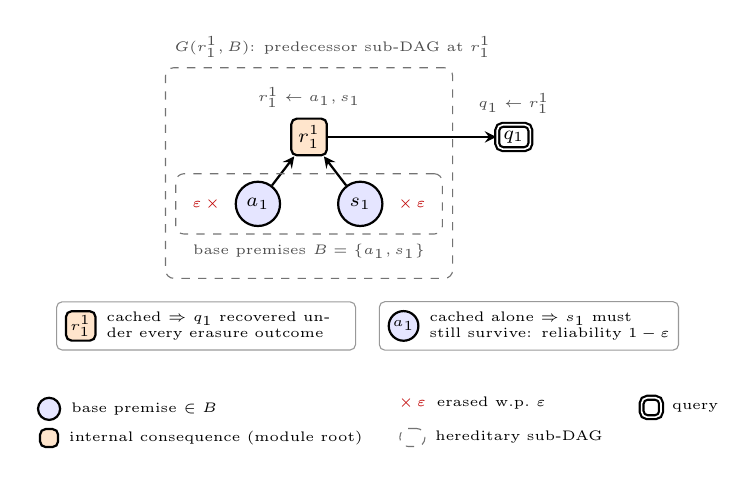
\begin{tikzpicture}[
  font=\scriptsize,
  leaf/.style={circle,draw,thick,fill=blue!10,inner sep=1.2pt,minimum size=16pt},
  int/.style={rectangle,draw,thick,rounded corners=2pt,fill=orange!20,inner sep=2.5pt},
  query/.style={rectangle,draw,thick,rounded corners=2pt,double,inner sep=2.2pt},
  rl/.style={font=\tiny,text=black!70},
  reg/.style={draw=black!55,dashed,rounded corners=3pt},
  emark/.style={font=\tiny,text=red!75!black},
  chipbox/.style={draw=black!40,rounded corners=2pt,inner sep=3pt},
  ctext/.style={font=\tiny,anchor=west,inner sep=0pt,align=left},
  >=stealth]
% ---- witness DAG ----
\node[leaf] (a1) at (3.20,0.3) {\(a_{1}\)};
\node[leaf] (s1) at (4.50,0.3) {\(s_{1}\)};
\node[int]  (r1) at (3.85,1.15) {\(r_{1}^{1}\)};
\node[query] (q1) at (6.45,1.15) {\(q_{1}\)};
\draw[->,thick] (a1) -- (r1);
\draw[->,thick] (s1) -- (r1);
\draw[->,thick] (r1) -- (q1);
% rule annotations (= designated parent tuples)
\node[rl, anchor=south] (rlr) at (r1.north) {\(r_{1}^{1}\leftarrow a_{1},s_{1}\)};
\node[rl, anchor=south] (rlq) at (q1.north) {\(q_{1}\leftarrow r_{1}^{1}\)};
% erasure marks on base premises
\node[emark, anchor=east] (em1) at ($(a1.west)+(-0.6mm,0)$) {\(\varepsilon\,\times\)};
\node[emark, anchor=west] (em2) at ($(s1.east)+(0.6mm,0)$) {\(\times\,\varepsilon\)};
% regions: base set B and hereditary sub-DAG G(r_1^1,B)
\node[reg, inner sep=2.5pt, fit=(a1)(s1)(em1)(em2)] (bbox) {};
\node[font=\tiny, text=black!70, anchor=north] (blab) at (bbox.south)
  {base premises \(B=\{a_{1},s_{1}\}\)};
\node[reg, inner sep=3.5pt, fit=(blab)(bbox)(r1)(rlr)] (gbox) {};
\node[font=\tiny, text=black!70, anchor=south west] at (gbox.north west)
  {\(G(r_{1}^{1},B)\): predecessor sub-DAG at \(r_{1}^{1}\)};
% ---- cache-scenario chips ----
\node[int, inner sep=1.6pt, minimum size=0pt, font=\tiny] (c1i) at (0.95,-1.25) {\(r_{1}^{1}\)};
\node[ctext, text width=3.05cm] (c1t) at ($(c1i.east)+(1.2mm,0)$)
  {cached \(\Rightarrow\) \(q_{1}\) recovered under every erasure outcome};
\node[chipbox, fit=(c1i)(c1t)] {};
\node[leaf, inner sep=0.8pt, minimum size=9pt, font=\tiny] (c2i) at (5.05,-1.25) {\(a_{1}\)};
\node[ctext, text width=3.05cm] (c2t) at ($(c2i.east)+(1.2mm,0)$)
  {cached alone \(\Rightarrow\) \(s_{1}\) must still survive: reliability \(1-\varepsilon\)};
\node[chipbox, fit=(c2i)(c2t)] {};
% ---- legend ----
\matrix[anchor=north, row sep=2.5pt, column sep=13pt, every node/.style={inner sep=0pt}]
  at (4.72,-2.0)
{
  \node[leaf, minimum size=8pt, inner sep=0.6pt,
        label={[font=\tiny,text=black,label distance=1.2mm]right:base premise \(\in B\)}] {}; &
  \node[font=\tiny, text=red!75!black,
        label={[font=\tiny,text=black,label distance=1.2mm]right:erased w.p.\ \(\varepsilon\)}] {\(\times\,\varepsilon\)}; &
  \node[query, minimum size=7pt, inner sep=0.9pt,
        label={[font=\tiny,text=black,label distance=1.2mm]right:query}] {}; \\
  \node[int, minimum size=6.5pt, inner sep=1pt,
        label={[font=\tiny,text=black,label distance=1.2mm]right:internal consequence (module root)}] {}; &
  \node[reg, minimum width=9pt, minimum height=6.5pt,
        label={[font=\tiny,text=black,label distance=1.2mm]right:hereditary sub-DAG}] {}; & \\
};
\end{tikzpicture}
\caption{The canonical DAG \(G(q_{1},B)\) of
Example~\ref{ex:minimal-canonical}.  The Datalog rules annotate the derived
nodes they produce, so each edge reads as a designated-parent relation.
Circles are base premises, each erased independently with probability
\(\varepsilon\) (red marks); rounded rectangles are derived nodes; the
doubled rectangle is the query.  The inner dashed region is the base set
\(B\); the outer one is the predecessor sub-DAG \(G(r_{1}^{1},B)\) of the
hereditary identity \eqref{eq:hereditary-subdag}.  The module root
\(r_{1}^{1}\) postdominates both premises, and the lower chips contrast the
two cache placements of the example: caching \(r_{1}^{1}\) recovers
\(q_{1}\) under every erasure outcome, whereas caching only \(a_{1}\)
leaves \(s_{1}\) as the residual leaf, with reliability \(1-\varepsilon\).}
\label{fig:datalog-witness}
\end{figure}

\begin{remark}[Typicality and interpretation of the canonical regime]
\label{rem:exact-scope}
Assumptions~\ref{assump:det-local} and~\ref{assump:hereditary-dag} are not
universal laws of reasoning systems; they describe the regime obtained after
one admissible derivation, proof skeleton, rule instance, or query plan has
been fixed, as in acyclic single-rule Horn fragments, compiled deterministic query
plans, and provenance systems with a designated derivation.  Within this
regime a cached consequence has an unambiguous meaning, whereas a base
premise remains usable only if it survives the erasures or is itself stored.
\end{remark}

\begin{remark}[Why these assumptions matter, and how they may be relaxed]
\label{rem:assumption-roles}
Assumption~\ref{assump:det-local} supplies the local availability
recursion, the source of direct cache availability and of the all-parent
failure recursion.  Assumption~\ref{assump:hereditary-dag} supplies
finiteness, acyclicity, and rooted hereditary structure, which enable
induction on the canonical DAG and make rooted semantic modules independent
of the ambient query.  The hereditary identity \eqref{eq:hereditary-subdag}
is stronger than a purely single-query analysis requires; it becomes
essential once internal consequences are reused across a workload.  The
natural relaxation---several admissible parent tuples per conclusion,
replacing the canonical DAG by an AND--OR provenance graph---is carried out
in Subsection~\ref{subsec:envelope-nonunique}; if heredity fails, a rooted
module may still help, but its meaning must then be indexed by the ambient
query.
\end{remark}

\subsection{Premise Erasures and Transparent Cache Classes}
\label{subsec:erasure-cache-model}

Each premise is independently erased with probability
\(\varepsilon\in(0,1)\).  Let
\[
  Z_i\sim\operatorname{Bernoulli}(1-\varepsilon),
  \qquad i=1,\ldots,m,
\]
be independent survival indicators and define the surviving premise set
\[
  \widetilde B
  :=
  \{b_i\in B:Z_i=1\}.
\]
All probabilities below refer to this erasure process unless stated
otherwise.

A query-dependent transparent cache policy is a mapping
\[
  S:\mathcal Q\longrightarrow
  \bigl\{\text{finite subsets of }\Cn(B)\bigr\},
  \qquad q\longmapsto S(q),
\]
chosen before the erasure realization.  Transparency means that every stored
object is an explicit consequence in \(\Cn(B)\), not an arbitrary parity
string or an opaque coded symbol.  For a fixed query \(q\), we often
abbreviate \(S(q)\) by \(S\).

Recovery of \(q\) succeeds exactly on the event
\[
  q\in\Cn\bigl(\widetilde B\cup S(q)\bigr).
\]
The cache is \((\varepsilon,\delta)\)-reliable for \(q\) if
\[
  \Pr_{\varepsilon}\!\left[
    q\in\Cn\bigl(\widetilde B\cup S(q)\bigr)
  \right]
  \ge 1-\delta,
  \qquad \delta\in(0,1).
\]

Fix an explicit-object cost function
\[
  c:\Cn(B)\longrightarrow\mathbb R_{>0},
\]
where \(c(v)\) is the storage cost of the object \(v\) itself in that unit,
including its self-delimiting representation.  Identifiers in
the system metadata do not count as stored copies of the corresponding
payloads.  For a finite set \(S\subseteq\Cn(B)\), define
\(\ell_c(S):=\sum_{v\in S}c(v)\).

A transparent cache may in principle contain the requested answer itself.
Such \emph{direct-answer caching} is reported as a separate baseline.  The
main structural results instead use the answer-excluding class
\(q\notin S(q)\) for a single query and \(S_W\cap W=\varnothing\) for a
workload \(W\).  This convention keeps ordinary result caching separate
from storage gains obtained by reusing internal derivation structure.

For a workload
\[
  W=\{q_1,\ldots,q_L\}\subseteq\mathcal Q,
\]
a common transparent cache \(S_W\subseteq\Cn(B)\) is \emph{jointly}
\((\varepsilon,\delta)\)-reliable if
\begin{equation}
  \Pr_{\varepsilon}\!\left[
    \bigcap_{\ell=1}^{L}
    \left\{
      q_\ell\in\Cn(\widetilde B\cup S_W)
    \right\}
  \right]
  \ge 1-\delta,
\label{eq:model-joint-criterion}
\end{equation}
and it is \emph{maximal-error} \((\varepsilon,\delta)\)-reliable if
\begin{equation}
  \Pr_{\varepsilon}\!\left[
    q_\ell\in\Cn(\widetilde B\cup S_W)
  \right]
  \ge 1-\delta,
  \qquad \ell=1,\ldots,L.
\label{eq:model-max-criterion}
\end{equation}
The joint criterion constrains one intersection event; the maximal-error
criterion constrains each marginal recovery event separately.  Joint
reliability therefore implies maximal-error reliability for any fixed cache.

Three workload-level cache classes will be compared.

\begin{itemize}[leftmargin=5mm]
\item A \emph{leaf-only transparent cache} is restricted to \(S_W\subseteq B\).

\item A \emph{semantic-aware transparent cache} may additionally store internal
consequences in \(\Cn(B)\), including roots of shared canonical sub-DAGs.

\item An \emph{unrestricted coded cache} may store arbitrary binary functions
of the premise payloads.
\end{itemize}

Under a fixed workload, a fixed answer-exclusion convention, and a fixed
reliability criterion, the corresponding optimal storage costs are denoted by
\[
  \sigma_{\mathrm{leaf}}^*(W,\varepsilon,\delta),\qquad
  \sigma_{\mathrm{sem}}^*(W,\varepsilon,\delta),\qquad
  \sigma_{\mathrm{code}}^*(W,\varepsilon,\delta),
\]
respectively.  These are the workload-level optima of
\eqref{eq:intro-three-way}, and they inherit its class-inclusion ordering:
every leaf-only cache is transparent, and every transparent cache is a
degenerate coded cache, since each stored consequence is a computable
function of the premise payloads.

When the distinction between the joint and maximal-error workload criteria
must be made explicit, we write
\[
  \sigma_{\bullet}^{*,\mathrm{joint}}(W,\varepsilon,\delta)
  \qquad\text{and}\qquad
  \sigma_{\bullet}^{*,\max}(W,\varepsilon,\delta),
\]
respectively, where
\[
  \bullet\in\{\mathrm{leaf},\mathrm{sem},\mathrm{code}\}.
\]
When the reliability criterion is fixed by context, we revert to the shorter
notation used above.

\subsection{Standing Notation and the Survival Threshold}
\label{subsec:standing-notation}

For \(x\in\mathbb R\), write \(x^+:=\max\{x,0\}\).

For a fixed query \(q\in\mathcal Q\), we will frequently abbreviate
\(G_q:=G(q,B)\), \(V_0(G_q):=V(G_q)\cap B\), and
\(\kappa_q:=|V_0(G_q)|\); for a workload
\(W=\{q_1,\ldots,q_L\}\subseteq\mathcal Q\), we also write
\(G_\ell:=G(q_\ell,B)\) and \(D_\ell:=V_0(G_\ell)\).

A recurring reliability threshold is
\begin{equation}
  \begin{split}
    N^*(\varepsilon,\delta)
    :=& \max\Bigl\{  n\in\mathbb Z_{\ge 0}: \\
    & (1-\varepsilon)^n \ge 1-\delta \Bigr\}
    = \left\lfloor \frac{\log(1-\delta)}{\log(1-\varepsilon)} \right\rfloor.
  \end{split}
\label{eq:model-N-star}
\end{equation}
This is the largest integer \(n\) for which the simultaneous survival of
\(n\) independently erased premises still has probability at least
\(1-\delta\).  Its operational meaning is fixed by the following baseline
law.

\begin{proposition}[Native survival law]
\label{prop:native-survival}
Under Assumptions~\ref{assump:det-local} and~\ref{assump:hereditary-dag}, for
every \(q\in\mathcal Q\setminus B\),
\begin{equation}
  \Pr_{\varepsilon}\!\left[q\in\Cn(\widetilde B)\right]
  =
  (1-\varepsilon)^{\kappa_q}.
\label{eq:native-survival}
\end{equation}
Consequently, recovery without any cache is \((\varepsilon,\delta)\)-reliable
if and only if
\begin{equation}
  \kappa_q\le N^*(\varepsilon,\delta).
\label{eq:nstar-threshold}
\end{equation}
\end{proposition}

\begin{proof}
For a base vertex \(v\in B\), \eqref{eq:base-irreducibility} gives
\(v\in\Cn(\widetilde B)\Leftrightarrow v\in\widetilde B\).
For a non-leaf vertex \(v\in V(G_q)\setminus B\),
\eqref{eq:deterministic-local-law} applied recursively downward along the
finite acyclic graph \(G_q[v]\) gives
\[
  v\in\Cn(\widetilde B)
  \quad\Longleftrightarrow\quad
  V_0(G_q[v])\subseteq\widetilde B.
\]
Applying this at \(v=q\) yields
\(q\in\Cn(\widetilde B)\Leftrightarrow V_0(G_q)\subseteq\widetilde B\), and
\eqref{eq:native-survival} follows from independence of the survival
indicators since \(|V_0(G_q)|=\kappa_q\).  The threshold form
\eqref{eq:nstar-threshold} is then immediate from \eqref{eq:model-N-star}.
\end{proof}

\subsection{Auxiliary Coded-Benchmark Layer}
\label{subsec:coded-benchmark-layer}

The transparent cache classes above restrict what may be stored.  To price
these restrictions, we compare them against an unrestricted coded reference
system.  Throughout this benchmark layer, every relevant base
premise carries a \(c_B\)-bit payload, regarded as one symbol of a payload
alphabet \(\mathcal X\) of size \(2^{c_B}\).  Stored benchmark strings are
not subject to erasure.

\begin{definition}[Auxiliary leaf-payload erasure channel]
\label{def:leaf-payload-channel}
Let \(A\subseteq B\) be a finite family of \(n:=|A|\) premises with payloads
\(X^n=(X_b)_{b\in A}\in\mathcal X^n\).  The auxiliary observation is
\[
  Y^n=(Y_b)_{b\in A},
  \qquad
  Y_b=
  \begin{cases}
    X_b, & Z_b=1,\\
    \bot, & Z_b=0,
  \end{cases}
\]
so that, conditionally on the payloads, each coordinate is independently
revealed with probability \(1-\varepsilon\) and erased with probability
\(\varepsilon\).
\end{definition}

\begin{definition}[Coded outer-benchmark task]
\label{def:coded-benchmark-task}
For a family \(A\subseteq B\) as above, a \emph{coded benchmark scheme}
\((\Enc,\Dec,\sigma)\) consists of computable maps
\[
  \Enc:\mathcal X^{n}\longrightarrow\{0,1\}^{\sigma},
  \;
  \Dec:\bigl(\mathcal X\cup\{\bot\}\bigr)^{n}\times\{0,1\}^{\sigma}
  \longrightarrow\mathcal X^{n}.
\]
The cache string \(T=\Enc(X^{n})\) is produced before the erasure realization.
The scheme is \(\delta\)-reliable for \(A\) if, for every payload realization,
\[
  \Pr\!\left[\Dec(Y^{n},T)=X^{n}\right]\ge 1-\delta,
\]
with probability taken over the erasure process.  The minimum admissible
\(\sigma\) is denoted \(\bar\sigma_{\mathrm{code}}(A,\varepsilon,\delta)\).
\end{definition}

\begin{remark}[The benchmark is auxiliary and strictly stronger than query recovery]
\label{rem:benchmark-honesty}
Two features of Definitions~\ref{def:leaf-payload-channel}
and~\ref{def:coded-benchmark-task} are kept explicit throughout the paper.
First, the channel \(Y^{n}\) retains the erased-or-revealed dependent
payloads and discards the rest of the surviving premise set \(\widetilde B\).
It is an auxiliary Shannon-style benchmark in the classical erasure-coding
sense \cite{cover2006elements,polyanskiy2010channel}, not a claimed
conditional-independence decomposition of \(\widetilde B\).
Second, the benchmark reconstructs \emph{all} dependent payloads.  This is
strictly stronger than answering any particular query: every query whose leaf
set lies in \(A\) can be evaluated once the payloads of \(A\) have been
reconstructed.  Hence, for the workload dependency union
\(D_{\mathrm{dep}}(W)\) defined in Section~\ref{sec:coded-outer},
\[
  \sigma_{\mathrm{code}}^{*}(W,\varepsilon,\delta)
  \;\le\;
  \bar\sigma_{\mathrm{code}}
  \bigl(D_{\mathrm{dep}}(W),\varepsilon,\delta\bigr),
\]
so the benchmark is an explicit, architecture-independent \emph{outer}
reference point.  The benchmark overstates what the coded side must achieve,
so benchmark-relative overhead numbers \emph{lower-bound} the price of
semantic transparency: the true coded optimum can only lie lower, and the
true transparency price can only be larger.
\end{remark}

\begin{remark}[Exactness convention and claim boundary]
\label{rem:exactness-convention}
Throughout the paper, a statement is called \emph{exact} only if it is a
closed-form identity or a finite-dimensional optimization that holds for
every instance of the stated regime, without uncontrolled approximation.
Three boundaries are fixed once and for all.  First, every exact statement
about transparent caches is made under Assumptions~\ref{assump:det-local}
and~\ref{assump:hereditary-dag} and under the answer-exclusion convention of
Subsection~\ref{subsec:erasure-cache-model}.  The only relaxation is the
envelope extension of Subsection~\ref{subsec:envelope-nonunique}, and it is
labeled as a relaxation wherever it is used.  Second, every quantitative
statement about coded storage---the MDS parity threshold, its
near-optimality, the strong converse, and the overhead laws---concerns the
explicit benchmark task of Definition~\ref{def:coded-benchmark-task}.  The
benchmark optimum \(\bar\sigma_{\mathrm{code}}\) upper-bounds the
unrestricted coded optimum \(\sigma_{\mathrm{code}}^{*}\), which is not
identified in this paper.  By Remark~\ref{rem:benchmark-honesty},
benchmark-relative overhead statements therefore lower-bound the true price
of transparency.  Third, asymptotic statements always carry their regime:
\(\kappa\to\infty\) at fixed \((\varepsilon,\delta)\) for the overhead laws,
or the alphabet-growth regime of Section~\ref{sec:coded-outer} for the
strong-converse exponent.  All other statements are finite-parameter
statements in the sense above.
\end{remark}

%%%%%%%%%%%%%%%%%%%%%%%%%%%%%%%%%%%%%%%%%%%%%%%%%%%%%%%%%%%%%%%%%%%%%%%%%%%%%%%%
%%% Section III
%%%%%%%%%%%%%%%%%%%%%%%%%%%%%%%%%%%%%%%%%%%%%%%%%%%%%%%%%%%%%%%%%%%%%%%%%%%%%%%%
\section{Exact Single-Query Structural Kernel}
\label{sec:single-query-kernel}

This section establishes the exact single-query recovery law.  It is the
structural kernel for the workload and coded analyses of
Sections~\ref{sec:semantic-scenario}--\ref{sec:coded-outer}.  Fix a non-base
query \(q\in\mathcal Q\setminus B\) and retain the standing notation
\(G_q\), \(V_0(G_q)\), and \(\kappa_q\) of
Subsection~\ref{subsec:standing-notation}.
All statements in this section are deterministic in the erasure realization
\(\widetilde B\subseteq B\).  Probability enters only after the exact
recovery event has been identified.

\subsection{Query-Local Projection and Failure Paths}
\label{subsec:query-local-projection}

\begin{definition}[Query-local projection and exposed leaves]
\label{def:query-local-residual}
For a finite transparent cache \(S\subseteq\Cn(B)\), define its projection onto
the canonical query DAG by
\begin{equation}
  U(q,S):=S\cap V(G_q).
\label{eq:query-local-projection}
\end{equation}
For each \(b\in V_0(G_q)\), let \(\mathcal P_q(b)\) denote the set of all
directed paths from \(b\) to \(q\) in \(G_q\), each path being identified
with its vertex set, endpoints included.

A path \(P\in\mathcal P_q(b)\) is \emph{cache-free} if
\[
  V(P)\cap U(q,S)=\varnothing.
\]
The residual exposed-leaf set is
\begin{equation}
  \begin{split}
    D_{\mathrm{exp}}(q,&S)
    := \bigl\{ b\in V_0(G_q) :  \\
    & \exists P\in\mathcal P_q(b) \text{ such that }
      V(P)\cap U(q,S)=\varnothing \bigr\}.
  \end{split}
\label{eq:def-exposed-leaves}
\end{equation}
Its complement
\begin{equation}
  D_{\mathrm{blk}}(q,S)
  :=
  V_0(G_q)\setminus D_{\mathrm{exp}}(q,S)
\label{eq:def-blocked-leaves}
\end{equation}
is the set of base leaves whose every path to \(q\) intersects the query-local
cache.
\end{definition}

The path quantifier in Definition~\ref{def:query-local-residual} is
essential.  In a general DAG, a base leaf may reach \(q\) through a cached
internal vertex along one path and bypass it along another.  Such a leaf
remains exposed.

\begin{lemma}[Failure-path characterization]
\label{lem:failure-path}
Under Assumptions~\ref{assump:det-local} and
\ref{assump:hereditary-dag}, let \(S\subseteq\Cn(B)\) be finite,
\(U:=U(q,S)\), and \(v\in V(G_q)\).  Then
\begin{align}
  v\notin\Cn(\widetilde B\cup U)
  \Longleftrightarrow
  &\ \exists b\in V_0(G_q[v])\setminus\widetilde B
  \nonumber\\[-1mm]
  &\ \exists\text{ a directed path \(P:b\leadsto v\) in \(G_q[v]\)}
  \nonumber\\[-1mm]
  &\text{such that }V(P)\cap U=\varnothing.
\label{eq:failure-path}
\end{align}
\end{lemma}

\begin{proof}
We argue by induction along a topological ordering of \(G_q[v]\), equivalently
on the predecessor depth of the terminal vertex.

First consider the base case \(v\in B\).  By the base-irreducibility law
\eqref{eq:base-irreducibility},
\(v\in\Cn(\widetilde B\cup U)\Leftrightarrow v\in\widetilde B\cup U\), hence
\(v\notin\Cn(\widetilde B\cup U)\Leftrightarrow v\notin\widetilde B\) and
\(v\notin U\).
Since \(G_q[v]\) is the singleton graph on \(v\), this is equivalent to the
existence of the length-zero path \(P=(v)\), which is cache-free and starts at
the missing base leaf \(b=v\).  This proves \eqref{eq:failure-path} when
\(v\in B\).

Now let \(v\in V(G_q)\setminus B\), and assume the statement holds for all
strict predecessors of \(v\) in \(G_q[v]\).  If \(v\in U\), then
\(v\in\Cn(\widetilde B\cup U)\) by direct availability, so the left-hand side
of \eqref{eq:failure-path} is false.  The right-hand side is also false,
because every directed path ending at \(v\) contains \(v\in U\) and therefore
cannot be cache-free.

Suppose next that \(v\notin U\), and write
\(\operatorname{par}(v)=(u_1,\ldots,u_{a(v)})\).
Since \(v\notin B\), one has \(v\notin\widetilde B\), and therefore
\eqref{eq:deterministic-local-law} gives
\begin{equation}
  \begin{aligned}
    & v\notin\Cn(\widetilde B\cup U) \\
    & \quad\Longleftrightarrow\quad 
      \exists\, i\in\{1,\ldots,a(v)\},\ 
      u_i\notin\Cn(\widetilde B\cup U).
  \end{aligned}
\label{eq:parent-failure-recursion}
\end{equation}
By Assumption~\ref{assump:hereditary-dag}, the in-neighborhood of \(v\) in
\(G_q[v]\) is exactly \(\{u_1,\ldots,u_{a(v)}\}\).  Thus every such \(u_i\) is
a strict predecessor of \(v\), and the induction hypothesis applies to \(u_i\).
If some \(u_i\notin\Cn(\widetilde B\cup U)\), then there exist
\(b\in V_0(G_q[u_i])\setminus\widetilde B\) and a cache-free directed path
\(P':b\leadsto u_i\) in \(G_q[u_i]\).  Appending the edge \((u_i,v)\) yields a
cache-free directed path \(P:b\leadsto v\) in \(G_q[v]\), proving the
right-hand side of \eqref{eq:failure-path}.

Conversely, suppose there exist
\(b\in V_0(G_q[v])\setminus\widetilde B\) and a cache-free directed path
\(P:b\leadsto v\) in \(G_q[v]\).  Since \(v\notin U\), the final edge of \(P\)
must be \((u_i,v)\) for some parent \(u_i\in\operatorname{par}(v)\).  The
prefix of \(P\) from \(b\) to \(u_i\) is again cache-free, so the induction
hypothesis implies \(u_i\notin\Cn(\widetilde B\cup U)\).  Equation
\eqref{eq:parent-failure-recursion} then yields
\(v\notin\Cn(\widetilde B\cup U)\).
\end{proof}

\begin{theorem}[Query-local rigidity and exact residual-leaf law]
\label{thm:exact-residual-law}
Under Assumptions~\ref{assump:det-local} and
\ref{assump:hereditary-dag}, for every finite
\(S\subseteq\Cn(B)\) and every \(\widetilde B\subseteq B\),
\begin{align}
  q\in\Cn(\widetilde B\cup S)
  &\Longleftrightarrow
  q\in\Cn\bigl(\widetilde B\cup U(q,S)\bigr),
\label{eq:query-local-rigidity}\\
  &\Longleftrightarrow
  D_{\mathrm{exp}}(q,S)\subseteq\widetilde B.
\label{eq:exact-residual-event}
\end{align}
Consequently, under independent premise erasures with erasure probability
\(\varepsilon\),
\begin{equation}
  \Pr_{\varepsilon}
  \left[
    q\in\Cn(\widetilde B\cup S)
  \right]
  =
  (1-\varepsilon)^{|D_{\mathrm{exp}}(q,S)|}.
\label{eq:exact-residual-probability}
\end{equation}
\end{theorem}

\begin{proof}
Let \(A_S:=\widetilde B\cup S\) and \(A_U:=\widetilde B\cup U(q,S)\).
We first show, by induction on a topological ordering of \(G_q\), that every
vertex \(v\in V(G_q)\) has the same availability under \(A_S\) and \(A_U\).

If \(v\in V_0(G_q)\), then \eqref{eq:base-irreducibility} implies
\(v\in\Cn(A_S)\Leftrightarrow v\in A_S\) and
\(v\in\Cn(A_U)\Leftrightarrow v\in A_U\).  Because \(v\in V(G_q)\),
\(v\in S\Leftrightarrow v\in U(q,S)\), and hence \(v\in A_S\) if and only if
\(v\in A_U\); therefore \(v\in\Cn(A_S)\Leftrightarrow v\in\Cn(A_U)\) for
every base leaf \(v\in V_0(G_q)\).

Now let \(v\in V(G_q)\setminus B\), and assume the equivalence has already been
proved for all strict predecessors of \(v\) in \(G_q\).  Since \(v\notin B\),
direct membership in \(A_S\) and \(A_U\) is equivalent to direct storage, and
again \(v\in S\Leftrightarrow v\in U(q,S)\).  Write
\(\operatorname{par}(v)=(u_1,\ldots,u_{a(v)})\).  By
\eqref{eq:deterministic-local-law},
\(v\in\Cn(A_S)\Leftrightarrow[v\in S\ \text{or}\
\{u_1,\ldots,u_{a(v)}\}\subseteq\Cn(A_S)]\),
and similarly with \(A_U\) and \(U(q,S)\) in place of \(A_S\) and \(S\).
The direct-storage terms agree, and all parent vertices \(u_i\) belong to
\(G_q\) and satisfy the induction hypothesis; hence
\(v\in\Cn(A_S)\Leftrightarrow v\in\Cn(A_U)\).
Applying this to \(v=q\) proves \eqref{eq:query-local-rigidity}.

For \eqref{eq:exact-residual-event}, apply
Lemma~\ref{lem:failure-path} with terminal vertex \(v=q\).  Since
\(V_0(G_q[q])=V_0(G_q)\), the complement of the recovery event
\(q\in\Cn(\widetilde B\cup U(q,S))\)
occurs exactly when there exists a missing base leaf
\(b\in V_0(G_q)\setminus\widetilde B\) having a cache-free directed path to
\(q\).  By Definition~\ref{def:query-local-residual}, this is equivalent to
\(D_{\mathrm{exp}}(q,S)\nsubseteq\widetilde B\).
Taking complements yields \eqref{eq:exact-residual-event}.

Finally, once \(q\) and \(S\) are fixed, the set \(D_{\mathrm{exp}}(q,S)\) is a
deterministic subset of the distinct base premises.  Under independent erasures,
the event \(D_{\mathrm{exp}}(q,S)\subseteq\widetilde B\) occurs if and only if
all premises in \(D_{\mathrm{exp}}(q,S)\) survive, which has probability
\((1-\varepsilon)^{|D_{\mathrm{exp}}(q,S)|}\).
Together with \eqref{eq:exact-residual-event}, this proves
\eqref{eq:exact-residual-probability}.
\end{proof}

\begin{corollary}[Exact reliability threshold]
\label{cor:exact-reliability-threshold}
Let \(N^*(\varepsilon,\delta)\) be defined by
\eqref{eq:model-N-star}.  A finite transparent cache \(S\) is
\((\varepsilon,\delta)\)-reliable for \(q\) if and only if
\begin{equation}
  |D_{\mathrm{exp}}(q,S)|
  \le
  N^*(\varepsilon,\delta).
\label{eq:exact-reliability-threshold}
\end{equation}
\end{corollary}

\begin{proof}
By \eqref{eq:exact-residual-probability}, reliability is equivalent to
\[
  (1-\varepsilon)^{|D_{\mathrm{exp}}(q,S)|}\ge 1-\delta.
\]
The claim is therefore immediate from the definition of
\(N^*(\varepsilon,\delta)\).
\end{proof}

\subsection{Path Interception and Query Postdominators}
\label{subsec:postdominator-interpretation}

Edges point from prerequisites toward consequences, and \(q\) is the
distinguished sink.  The relevant graph relation is therefore postdomination:
an internal vertex protects a leaf only when it lies on every path from that
leaf to \(q\).  Equivalently, it is a dominator relation in the
edge-reversed DAG \cite{lengauer1979fast}.

\begin{definition}[Query-postdominated leaf set]
\label{def:query-postdominator}
For an internal vertex
\(v\in V(G_q)\setminus(B\cup\{q\})\), define
\begin{equation}
  \operatorname{Pdom}_q(v)
  \!:=\!
  \bigl\{
    b\in V_0(G_q):
    v\in V(P)\ \forall P\in\mathcal P_q(b)
  \bigr\}.
\label{eq:def-query-postdominator}
\end{equation}
Thus \(v\) postdominates a base leaf \(b\) relative to the exit \(q\) if every
directed path from \(b\) to \(q\) contains \(v\).
\end{definition}

\begin{proposition}[Dependencies protected by an internal cache]
\label{prop:postdominator-protection}
For every internal
\(v\in V(G_q)\setminus(B\cup\{q\})\),
\begin{equation}
  D_{\mathrm{blk}}(q,\{v\})
  =
  \operatorname{Pdom}_q(v).
\label{eq:single-vertex-postdominator}
\end{equation}
More generally, for every finite \(S\subseteq\Cn(B)\),
\begin{equation}
  \begin{split}
    D_{\mathrm{blk}}(q,S)
    =
    &\bigl\{ b\in V_0(G_q) : \\
    & U(q,S)\cap V(P)\neq\varnothing \;\forall P\in\mathcal P_q(b) \bigr\}.
  \end{split}
\label{eq:set-path-interception}
\end{equation}
\end{proposition}

\begin{proof}
By Definition~\ref{def:query-local-residual}, \(b\in D_{\mathrm{blk}}(q,S)\)
holds exactly when no directed path from \(b\) to \(q\) is cache-free, namely,
when every path \(P\in\mathcal P_q(b)\) intersects \(U(q,S)\).  This proves
\eqref{eq:set-path-interception}.  Equation
\eqref{eq:single-vertex-postdominator} is the special case \(S=\{v\}\).
\end{proof}

\begin{remark}[Trees versus DAGs]
\label{rem:tree-versus-dag}
If \(G_q\) is a tree, every base leaf below \(v\) has a unique path to
\(q\), and therefore \(\operatorname{Pdom}_q(v)=V_0(G_q[v])\).  For a
general DAG only the inclusion
\(\operatorname{Pdom}_q(v)\subseteq V_0(G_q[v])\) is guaranteed, and it is
strict whenever a leaf of \(G_q[v]\) also reaches \(q\) along a path that
bypasses \(v\).  Internal semantic summaries must therefore be evaluated
through path interception or postdomination, not through sub-DAG membership
alone.
\end{remark}

\subsection{Exact Transparent-Storage Optimization}
\label{subsec:exact-storage-optimization}

A cache is \emph{answer-excluding} for \(q\) if it does not store \(q\)
itself (storing \(q\) directly is ordinary result caching: the optimum with
direct answers is simply
\(\min\{c(q),\sigma_{\mathrm{sem,int}}^*(q,\varepsilon,\delta)\}\), and
we keep this baseline separate so that gains from reusable derivation
structure are not conflated with it).  Define the corresponding optimum by
\begin{align}
  \sigma_{\mathrm{sem,int}}^*
  (q,\varepsilon,\delta)
  :=
  \min\Bigl\{
    &\ell_c(S):
    S\subseteq\Cn(B)\setminus\{q\},
    \ S\text{ finite},
    \nonumber\\[-1mm]
    &\Pr_{\varepsilon}
      \left[
        q\in\Cn(\widetilde B\cup S)
      \right]
      \ge 1-\delta
  \Bigr\}.
\label{eq:def-semantic-internal-optimum}
\end{align}

\begin{theorem}[Exact query-local storage formulation]
\label{thm:exact-single-query-opt}
Under Assumptions~\ref{assump:det-local} and
\ref{assump:hereditary-dag},
\begin{align}
  \sigma_{\mathrm{sem,int}}^*
  (q,\varepsilon,\delta)
  =
  \min\Bigl\{
    &\ell_c(S):
    S\subseteq V(G_q)\setminus\{q\},
    \nonumber\\[-1mm]
    &|D_{\mathrm{exp}}(q,S)|
      \le N^*(\varepsilon,\delta)
  \Bigr\}.
\label{eq:exact-single-query-opt}
\end{align}
Thus the answer-excluding single-query problem is exactly a weighted partial
path-interception problem: the cache must intercept every path from all but at
most \(N^*(\varepsilon,\delta)\) base leaves to \(q\).
\end{theorem}

\begin{proof}
By Corollary~\ref{cor:exact-reliability-threshold}, the reliability constraint
is equivalent to
\[
  |D_{\mathrm{exp}}(q,S)|\le N^*(\varepsilon,\delta).
\]

Now let \(S\subseteq\Cn(B)\setminus\{q\}\) be any feasible finite transparent
cache.  By Theorem~\ref{thm:exact-residual-law}, the projected cache \(U(q,S)\)
induces exactly the same recovery event.  Moreover,
\[
  U(q,S)\subseteq S
  \qquad\text{and}\qquad
  \ell_c\bigl(U(q,S)\bigr)\le \ell_c(S),
\]
because all object costs are strictly positive.  Hence every feasible cache can
be replaced, without hurting reliability and without increasing cost, by a
feasible cache contained in \(V(G_q)\setminus\{q\}\).  Conversely, every cache
contained in \(V(G_q)\setminus\{q\}\) is an admissible transparent cache.
This proves \eqref{eq:exact-single-query-opt}.
\end{proof}

\begin{corollary}[Exact leaf-only transparent baseline]
\label{cor:leaf-only-opt}
Restrict the cache to
\[
  S\subseteq V_0(G_q),
\]
and arrange the leaf costs in nondecreasing order:
\[
  c_{(1)}\le c_{(2)}\le\cdots\le c_{(\kappa_q)}.
\]
Then
\begin{equation}
  \sigma_{\mathrm{leaf}}^*
  (q,\varepsilon,\delta)
  =
  \sum_{i=1}^{(\kappa_q-N^*)^+}c_{(i)},
\label{eq:heterogeneous-leaf-opt}
\end{equation}
where
\(N^*=N^*(\varepsilon,\delta)\) and an empty sum equals zero.

If all base premises have the same explicit storage cost \(c_B\), then
\begin{equation}
  \sigma_{\mathrm{leaf}}^*
  (q,\varepsilon,\delta)
  =
  \bigl(\kappa_q-N^*(\varepsilon,\delta)\bigr)^+c_B.
\label{eq:homogeneous-leaf-opt}
\end{equation}
\end{corollary}

\begin{proof}
Let \(S\subseteq V_0(G_q)\).  Every base leaf is a source of \(G_q\), so a
directed path originating at one base leaf cannot pass through a distinct base
leaf.  Consequently, a leaf \(b\in V_0(G_q)\) is blocked by a leaf-only cache
if and only if \(b\in S\), so
\(D_{\mathrm{exp}}(q,S)=V_0(G_q)\setminus S\) and
\(|D_{\mathrm{exp}}(q,S)|=\kappa_q-|S|\).
By Corollary~\ref{cor:exact-reliability-threshold}, reliability is equivalent
to \(\kappa_q-|S|\le N^*(\varepsilon,\delta)\), i.e.\
\(|S|\ge(\kappa_q-N^*(\varepsilon,\delta))^+\).
Therefore the optimal leaf-only policy is to cache exactly that many leaves of
smallest cost, which proves \eqref{eq:heterogeneous-leaf-opt}.  The homogeneous
formula \eqref{eq:homogeneous-leaf-opt} follows immediately.
\end{proof}

\subsection{Semantic Modules and a Strict Single-Query Gain}
\label{subsec:single-query-module-benchmark}

Let
\[
  R=\{r_1,\ldots,r_M\}
  \subseteq
  V(G_q)\setminus(B\cup\{q\})
\]
be a selected set of internal semantic-module roots, and define
\begin{equation}
  p_R:=|D_{\mathrm{exp}}(q,R)|.
\label{eq:def-module-residual-count}
\end{equation}
Thus \(p_R\) is the number of base dependencies that remain exposed after all
vertices in \(R\) have been cached.

\begin{proposition}[Module roots followed by residual-leaf completion]
\label{prop:module-root-achievability}
For every
\[
  T\subseteq D_{\mathrm{exp}}(q,R),
\]
one has
\begin{equation}
  D_{\mathrm{exp}}(q,R\cup T)
  =
  D_{\mathrm{exp}}(q,R)\setminus T.
\label{eq:residual-after-leaf-completion}
\end{equation}
Consequently, if all base leaves have cost \(c_B\), then
\begin{equation}
  \sigma_{\mathrm{sem,int}}^*
  (q,\varepsilon,\delta)
  \le
  \sum_{j=1}^{M}c(r_j)
  +
  \bigl(p_R-N^*(\varepsilon,\delta)\bigr)^+c_B.
\label{eq:module-achievable-cost}
\end{equation}
\end{proposition}

\begin{proof}
Since \(T\subseteq V_0(G_q)\), every vertex of \(T\) is a base leaf.  We first
prove \eqref{eq:residual-after-leaf-completion}.

Adding more cached objects cannot create a new cache-free path, so
\(D_{\mathrm{exp}}(q,R\cup T)\subseteq D_{\mathrm{exp}}(q,R)\).
Moreover, each \(b\in T\) is blocked after being cached, because every directed
path from \(b\) to \(q\) contains its initial vertex \(b\); hence
\(D_{\mathrm{exp}}(q,R\cup T)\subseteq D_{\mathrm{exp}}(q,R)\setminus T\).

For the reverse inclusion, let \(b\in D_{\mathrm{exp}}(q,R)\setminus T\).  By
definition, there exists a directed path \(P\in\mathcal P_q(b)\) with
\(V(P)\cap R=\varnothing\).
Because \(T\) consists of base leaves and \(b\notin T\), the path \(P\) cannot
meet any vertex of \(T\): a directed path that starts at the source leaf \(b\)
cannot pass through a distinct source leaf.  Therefore
\(V(P)\cap(R\cup T)=\varnothing\), so \(b\in D_{\mathrm{exp}}(q,R\cup T)\).
This proves \eqref{eq:residual-after-leaf-completion}.

For the cost bound, cache the module roots in \(R\) together with any
\((p_R-N^*(\varepsilon,\delta))^+\)
leaves from the residual set \(D_{\mathrm{exp}}(q,R)\).  By
\eqref{eq:residual-after-leaf-completion}, the resulting exposed-leaf count is
at most \(N^*(\varepsilon,\delta)\).  Corollary~\ref{cor:exact-reliability-threshold}
therefore yields \eqref{eq:module-achievable-cost}.
\end{proof}

\begin{corollary}[Explicit sufficient condition for semantic gain]
\label{cor:explicit-semantic-gain}
Assume that
\(\operatorname{Pdom}_q(r_1),\ldots,\operatorname{Pdom}_q(r_M)\)
are pairwise disjoint with
\(|\operatorname{Pdom}_q(r_j)|\ge s\), \(j=1,\ldots,M\).
If \(c(r_j)=c_I\) for all \(j\), then
\begin{equation}
  p_R\le\kappa_q-Ms
\label{eq:module-residual-upper-bound}
\end{equation}
and
\begin{equation}
  \sigma_{\mathrm{sem,int}}^*
  (q,\varepsilon,\delta)
  \le
  Mc_I
  +
  \bigl(
    \kappa_q-Ms-N^*(\varepsilon,\delta)
  \bigr)^+c_B.
\label{eq:module-homogeneous-bound}
\end{equation}
Therefore the explicit module construction strictly improves on the
homogeneous leaf-only baseline whenever
\begin{align}
  Mc_I
  +
  \bigl(\kappa_q-Ms-N^*\bigr)^+c_B
  <
  \bigl(\kappa_q-N^*\bigr)^+c_B,
\label{eq:semantic-gain-condition}
\end{align}
where \(N^*=N^*(\varepsilon,\delta)\).

In particular, if
\[
  \kappa_q-Ms\ge N^*(\varepsilon,\delta),
\]
then the sufficient condition reduces to
\begin{equation}
  c_I<s\,c_B,
\label{eq:per-module-gain-condition}
\end{equation}
and the resulting saving relative to the leaf-only baseline is at least
\begin{equation}
  M\bigl(sc_B-c_I\bigr).
\label{eq:module-saving}
\end{equation}
\end{corollary}

\begin{proof}
By Proposition~\ref{prop:postdominator-protection}, caching \(r_j\) blocks
every leaf in \(\operatorname{Pdom}_q(r_j)\).  Hence
\[
  D_{\mathrm{blk}}(q,R)
  \supseteq
  \bigcup_{j=1}^{M}\operatorname{Pdom}_q(r_j).
\]
By pairwise disjointness and the cardinality assumption,
\[
  |D_{\mathrm{blk}}(q,R)|
  \ge
  \left|
    \bigcup_{j=1}^{M}\operatorname{Pdom}_q(r_j)
  \right|
  \ge Ms.
\]
Since
\[
  p_R
  =
  |D_{\mathrm{exp}}(q,R)|
  =
  \kappa_q-|D_{\mathrm{blk}}(q,R)|,
\]
equation \eqref{eq:module-residual-upper-bound} follows.  Substituting this
bound into Proposition~\ref{prop:module-root-achievability} gives
\eqref{eq:module-homogeneous-bound}.

The exact homogeneous leaf-only baseline is
\eqref{eq:homogeneous-leaf-opt}.  Therefore, whenever
\eqref{eq:semantic-gain-condition} holds, the displayed achievable
semantic-module cost is strictly smaller than the leaf-only optimum, and hence
so is \(\sigma_{\mathrm{sem,int}}^*(q,\varepsilon,\delta)\).

Finally, if \(\kappa_q-Ms\ge N^*\), then both positive-part terms in
\eqref{eq:semantic-gain-condition} are active, and their difference is
\(Ms\,c_B\).  This reduces the sufficient condition to
\eqref{eq:per-module-gain-condition} and yields the explicit saving lower bound
\eqref{eq:module-saving}.
\end{proof}

\begin{remark}[Set-wise interception can be stronger]
\label{rem:set-wise-interception}
For several cached vertices, the blocked set may strictly contain
\(\bigcup_{r\in R}\operatorname{Pdom}_q(r)\): different paths from one
leaf may be intercepted by different vertices of \(R\), even though no
single vertex lies on every path.  Thus
Corollary~\ref{cor:explicit-semantic-gain} is an easily checked sufficient
condition, not an exact characterization of the gain of a general module
set.
\end{remark}

\begin{remark}[Bridge to workload-level reuse]
\label{rem:bridge-to-workload}
The single-query gain above requires an internal consequence to cost less
than the raw premises it intercepts; a workload adds a second mechanism,
reuse, since one context-independent module is stored once but protects
several queried derivations at once.  The workload-level section specifies
the common cache, the reliability criterion, and the exact no-bypass
condition under which this happens.
\end{remark}

\subsection{Robustness to Non-Unique Derivations: An Envelope Law}
\label{subsec:envelope-nonunique}

Remark~\ref{rem:assumption-roles} flagged the relaxation in which a derived
object admits several admissible parent tuples instead of one designated
tuple.  The canonical DAG is then replaced by an AND--OR provenance structure
\cite{green2007provenance}.  This subsection carries out the relaxation for
the single-query kernel.  The exact residual law of
Theorem~\ref{thm:exact-residual-law} survives in an \emph{envelope} form:
recovery is an existential union over candidate witness DAGs, and its
probability is sandwiched between the best single witness and a union bound.
Throughout this subsection, Assumptions~\ref{assump:det-local} and
\ref{assump:hereditary-dag} are replaced by
Assumption~\ref{assump:and-or-local} below.  The standing notation of this
section, in particular the fixed query \(q\in\mathcal Q\setminus B\), is
retained.

\begin{assumption}[AND--OR local semantics with well-founded expansion]
\label{assump:and-or-local}
The operator \(\Cn\), with its closure axioms and effectiveness, and the
finite relevant region \(\mathcal V_{\mathrm{rel}}(B)\) are retained from
Assumption~\ref{assump:det-local}, as is the base-irreducibility law
\eqref{eq:base-irreducibility}; the designated-parent map, together with its
well-foundedness clause, is superseded by the admissible parent family below
and the rank condition \eqref{eq:well-founded-rank}.  The designated parent
map is replaced by a computable \emph{admissible parent family}: for every
\(v\in\mathcal V_{\mathrm{rel}}(B)\setminus B\),
\[
  \operatorname{Par}(v)
  \subseteq
  2^{\,\mathcal V_{\mathrm{rel}}(B)\setminus\{v\}}
\]
is a nonempty finite family of finite nonempty sets, and for every finite
\(\Gamma\subseteq\Cn(B)\),
\begin{equation}
  \begin{split}
    v & \in\Cn(\Gamma)
    \Longleftrightarrow
    \Bigl[ v\in\Gamma \;\lor \\
       & \exists P\in\operatorname{Par}(v):\, P\subseteq\Cn(\Gamma) \Bigr],
     v\in\mathcal V_{\mathrm{rel}}(B)\setminus B.
  \end{split}
\label{eq:and-or-local-law}
\end{equation}
Thus a derived object is available when it is stored or when \emph{at least
one} of its admissible parent tuples is fully derivable---an AND over each
tuple and an OR over the family.  Write \(r_v:=|\operatorname{Par}(v)|\),
and call \(v\) \emph{ambiguous} if \(r_v\ge 2\).
Assumption~\ref{assump:det-local} is the special case \(r_v=1\) for all
\(v\), with \(\operatorname{par}(v)\) the unique member of
\(\operatorname{Par}(v)\).

Finally, backward expansion is well-founded: there exists a rank function
\[
  \operatorname{rk}:\mathcal V_{\mathrm{rel}}(B)\longrightarrow\mathbb Z_{\ge0},
  \qquad
  \operatorname{rk}^{-1}(0)=B,
\]
such that
\begin{equation}
  u\in P\in\operatorname{Par}(v)
  \quad\Longrightarrow\quad
  \operatorname{rk}(u)<\operatorname{rk}(v).
\label{eq:well-founded-rank}
\end{equation}
\end{assumption}

\begin{definition}[Candidate witness DAGs and best-case residual]
\label{def:candidate-witness}
Let \(S\subseteq\Cn(B)\) be a finite transparent cache.  An \emph{\(S\)-relative
candidate witness DAG} for \(q\) is a finite acyclic digraph \(G\) with
\(V(G)\subseteq\mathcal V_{\mathrm{rel}}(B)\) and \(q\in V(G)\) such that:
\begin{enumerate}[label=\textup{(\roman*)}]
\item every vertex of \(G\) lies on a directed path terminating at \(q\);
\item every non-source vertex \(v\) has in-neighborhood
\(N_G^{-}(v)\in\operatorname{Par}(v)\);
\item every source of \(G\) lies in \(B\cup S\).
\end{enumerate}
A base vertex is always a source, since no admissible parent tuple is defined
on \(B\).  Denote the family of all such DAGs by \(\mathcal G_S(q,B)\), and
abbreviate the \emph{\(B\)-grounded} subfamily by
\[
  \mathcal G(q,B):=\mathcal G_{\varnothing}(q,B).
\]
Since \(\mathcal V_{\mathrm{rel}}(B)\) is finite, backward expansion from
\(q\) shows that
\begin{equation}
  |\mathcal G_S(q,B)|
  \le
  \prod_{v\in\mathcal V_{\mathrm{rel}}(B)\setminus B}(1+r_v)
  <\infty:
\label{eq:candidate-count-bound}
\end{equation}
at each visited non-base vertex, expansion either stops (permitted only at
\(B\cup S\)) or selects one of \(r_v\) admissible tuples, and distinct
expansions may yield the same DAG.  Moreover
\(\mathcal G(q,B)\neq\varnothing\) if and only if \(q\in\Cn(B)\): arbitrary
admissible choices strictly decrease the rank \eqref{eq:well-founded-rank},
hence terminate at rank zero, i.e.\ at \(B\); conversely, induction along any
\(B\)-grounded witness gives \(q\in\Cn(B)\).

For \(G\in\mathcal G_S(q,B)\), define
\[
  U_G(q,S):=S\cap V(G),
  \qquad
  V_0(G):=V(G)\cap B,
\]
and the exposed-leaf set
\begin{equation}
  \begin{split}
    D_{\mathrm{exp}}^{G}(q,S)
    := &\bigl\{ b\in V_0(G) :  \\
    & \exists\text{ a directed path }P:b\leadsto q\text{ in }G \\
    & \text{with }V(P)\cap U_G(q,S)=\varnothing \bigr\},
  \end{split}
\label{eq:def-exposed-leaves-witness}
\end{equation}
exactly as in Definition~\ref{def:query-local-residual} but with directed
paths taken in \(G\).  Write
\[
  e_G(q,S):=|D_{\mathrm{exp}}^{G}(q,S)|,
  \quad
  e_*(q,S):=\min_{G\in\mathcal G_S(q,B)}e_G(q,S).
\]
\end{definition}

\begin{theorem}[Envelope rigidity under non-unique derivations]
\label{thm:envelope-rigidity}
Under Assumption~\ref{assump:and-or-local}, suppose \(q\in\Cn(B)\) and let
\(S\subseteq\Cn(B)\) be finite.  Then:
\begin{enumerate}[label=\textup{(\alph*)}]
\item for every \(\widetilde B\subseteq B\),
\begin{equation}
  q\in\Cn(\widetilde B\cup S)
  \Longleftrightarrow
  \exists\,G\in\mathcal G_S(q,B):
  \ D_{\mathrm{exp}}^{G}(q,S)\subseteq\widetilde B;
\label{eq:envelope-event}
\end{equation}
equivalently, with survival indicators
\(X_b:=\mathbf 1\{b\in\widetilde B\}\), the recovery indicator is the
monotone DNF
\begin{equation}
  \mathbf 1\{q\in\Cn(\widetilde B\cup S)\}
  =
  \bigvee_{G\in\mathcal G_S(q,B)}
  \ \bigwedge_{b\in D_{\mathrm{exp}}^{G}(q,S)} X_b;
\label{eq:envelope-dnf}
\end{equation}
\item under independent premise erasures with erasure probability
\(\varepsilon\),
\begin{align}
  (1-\varepsilon)^{e_*(q,S)}
  &\le
  \Pr_{\varepsilon}\!\left[q\in\Cn(\widetilde B\cup S)\right]
  \nonumber\\
  &\le
  \min\!\left\{
    1,\;
    \sum_{G\in\mathcal G_S(q,B)}(1-\varepsilon)^{e_G(q,S)}
  \right\}
  \nonumber\\
  &\le
  \min\!\left\{
    1,\;
    |\mathcal G_S(q,B)|\,(1-\varepsilon)^{e_*(q,S)}
  \right\};
\label{eq:envelope-probability}
\end{align}
\item if the exposed sets
\(\{D_{\mathrm{exp}}^{G}(q,S)\}_{G\in\mathcal G_S(q,B)}\) are pairwise
disjoint, then exactly
\begin{equation}
  \Pr_{\varepsilon}\!\left[q\in\Cn(\widetilde B\cup S)\right]
  =
  1-\prod_{G\in\mathcal G_S(q,B)}
  \Bigl(1-(1-\varepsilon)^{e_G(q,S)}\Bigr);
\label{eq:envelope-independent}
\end{equation}
\item if \(r_v=1\) for every \(v\), then \(e_*(q,S)=|D_{\mathrm{exp}}(q,S)|\)
and the lower bound in \eqref{eq:envelope-probability} coincides with the
exact law \eqref{eq:exact-residual-probability}.
\end{enumerate}
\end{theorem}

\begin{proof}
(a)\ \emph{Sufficiency within a fixed witness.}
Fix \(G\in\mathcal G_S(q,B)\) and suppose
\(D_{\mathrm{exp}}^{G}(q,S)\subseteq\widetilde B\), yet
\(q\notin\Cn(\widetilde B\cup S)\).  Then \(q\notin S\), so \(q\) is not a
source of \(G\), and by \eqref{eq:and-or-local-law} applied with
\(P=N_G^{-}(q)\) some \(u_1\in N_G^{-}(q)\) satisfies
\(u_1\notin\Cn(\widetilde B\cup S)\).  Iterating, any unavailable non-source
vertex has an unavailable in-neighbor in \(G\); unavailable vertices cannot
belong to \(S\), and along edges the rank \eqref{eq:well-founded-rank}
strictly decreases, so the trace terminates at an unavailable source
\(b\).  A source in \(S\) would be available, and an unavailable base source
satisfies \(b\notin\widetilde B\cup S\) by \eqref{eq:base-irreducibility}.
Hence \(b\in B\setminus\widetilde B\), and the traced path
\(b\leadsto q\) meets no vertex of \(U_G(q,S)\), so
\(b\in D_{\mathrm{exp}}^{G}(q,S)\), contradicting
\(D_{\mathrm{exp}}^{G}(q,S)\subseteq\widetilde B\).

\emph{Extraction of a surviving witness.}
Conversely, suppose \(q\in\Cn(\widetilde B\cup S)\) and set
\(A:=\Cn(\widetilde B\cup S)\cap\mathcal V_{\mathrm{rel}}(B)\).  Expand
backward from \(q\): at a visited vertex \(v\in A\), stop if
\(v\in B\cup S\); otherwise \(v\notin\widetilde B\cup S\), and
\eqref{eq:and-or-local-law} with \(\Gamma=\widetilde B\cup S\) yields
\(P_v\in\operatorname{Par}(v)\) with \(P_v\subseteq\Cn(\widetilde B\cup S)\),
hence \(P_v\subseteq A\); continue from each \(u\in P_v\).  Edges strictly
decrease the rank, so the expansion is finite and acyclic, and every visited
vertex reaches \(q\) by construction.  The resulting \(G\) belongs to
\(\mathcal G_S(q,B)\).  Let \(b\in D_{\mathrm{exp}}^{G}(q,S)\) with a
cache-free path \(P:b\leadsto q\).  Walking backward along \(P\) from \(q\),
every internal vertex of \(P\) is a non-source of \(G\), hence was expanded
and lies in \(A\), and its predecessor on \(P\) lies in its chosen parent
tuple, hence also in \(A\).  Therefore \(b\in A\cap B\), so
\eqref{eq:base-irreducibility} gives \(b\in\widetilde B\cup S\); but
\(b\notin S\) since \(P\) is cache-free.  Thus
\(b\in\widetilde B\), proving
\(D_{\mathrm{exp}}^{G}(q,S)\subseteq\widetilde B\).  This completes
\eqref{eq:envelope-event}, and \eqref{eq:envelope-dnf} is a restatement.

(b)\ By \eqref{eq:envelope-event}, recovery is the union of the events
\(\{D_{\mathrm{exp}}^{G}(q,S)\subseteq\widetilde B\}\).  Each exposed set is
a deterministic subset of the distinct base premises, so each event has
probability \((1-\varepsilon)^{e_G(q,S)}\) exactly as in
Theorem~\ref{thm:exact-residual-law}.  The lower bound is the largest single
event probability, and the upper bounds are the union bound and
\(\sum_G(1-\varepsilon)^{e_G(q,S)}\le|\mathcal G_S(q,B)|\,
(1-\varepsilon)^{e_*(q,S)}\).

(c)\ Pairwise disjoint exposed sets make the survival events independent,
and the union probability evaluates to \eqref{eq:envelope-independent}.

(d)\ If \(r_v=1\) for all \(v\), write \(G_q\) for the unique \(B\)-grounded
witness.  Every \(S\)-relative candidate is obtained from \(G_q\) by deleting
the in-edges of a subset of the \(S\)-vertices and pruning vertices that no
longer reach \(q\): expansion is forced except that one may stop at
\(S\)-vertices.  Deleting fewer in-edges can only add directed paths, so the
exposed set is minimized by the full truncation \(T_q\), which deletes the
in-edges of every vertex in \(S\cap V(G_q)\).  The cache-free paths of
\(G_q\) are exactly the paths of \(T_q\) from base leaves to \(q\), so
\(e_*(q,S)=e_{T_q}(q,S)=|D_{\mathrm{exp}}(q,S)|\) with
\(D_{\mathrm{exp}}(q,S)\) as in
Definition~\ref{def:query-local-residual}, and the lower bound of
\eqref{eq:envelope-probability} equals
\eqref{eq:exact-residual-probability}.
\end{proof}

The exact probability is the probability of the DNF
\eqref{eq:envelope-dnf}.  It is computable by inclusion--exclusion over
\(\mathcal G_S(q,B)\), but in general at exponential cost in the family size.
The envelope \eqref{eq:envelope-probability} is the useful two-sided
compression, and it suffices for reliability design on the achievability
side.

Two consequences of the envelope law are used later in the paper; their
statements and proofs are collected in Appendix~\ref{app:envelope}.  First,
single-witness designs remain valid: if one candidate witness has
exposed-leaf count at most \(N^*(\varepsilon,\delta)\), then the cache is
\((\varepsilon,\delta)\)-reliable under the full AND--OR semantics, so every
achievable construction of Sections~\ref{sec:single-query-kernel}
and~\ref{sec:semantic-scenario} certifies reliability verbatim, at unchanged
cost (Corollary~\ref{cor:envelope-certified-threshold}).  Second, converses
survive with an additive slack: every storage lower bound of the canonical
regime remains valid after \(N^*\) is replaced by an inflated threshold
\(N^+_{\mathcal G}\le N^*+\Delta_{\mathcal G}+1\), where
\(\Delta_{\mathcal G}\) is logarithmic in the per-vertex derivation
multiplicities (Corollary~\ref{cor:envelope-relaxation-cost}).

%%%%%%%%%%%%%%%%%%%%%%%%%%%%%%%%%%%%%%%%%%%%%%%%%%%%%%%%%%%%%%%%%%%%%%%%%%%%%%%%%
%%% Section IV
%%%%%%%%%%%%%%%%%%%%%%%%%%%%%%%%%%%%%%%%%%%%%%%%%%%%%%%%%%%%%%%%%%%%%%%%%%%%%%%%%
\section{Semantic-Aware Transparent Caching for a Shared Workload}
\label{sec:semantic-scenario}

We now lift the single-query kernel of
Section~\ref{sec:single-query-kernel} to a common transparent cache that
serves a workload
\[
  W=\{q_1,\ldots,q_L\}\subseteq\mathcal Q
\]
over the same premise base \(B\).  For each \(\ell\), write
\[
  G_\ell:=G(q_\ell,B),
  \qquad
  D_\ell:=V_0(G_\ell),
  \qquad
  \kappa_\ell:=|D_\ell|.
\]
The two reliability conventions are recalled from
Subsection~\ref{subsec:erasure-cache-model}: under the maximal-error
criterion,
\[
  \Pr_\varepsilon\!\left[
    q_\ell\in\Cn(\widetilde B\cup S_W)
  \right]
  \ge 1-\delta,
  \qquad \ell=1,\ldots,L,
\]
whereas under the joint criterion,
\[
  \Pr_\varepsilon\!\left[
    \bigcap_{\ell=1}^{L}
    \{q_\ell\in\Cn(\widetilde B\cup S_W)\}
  \right]
  \ge 1-\delta.
\]

\subsection{Workload Projection and Exact Reliability Laws}
\label{subsec:workload-exact-laws}

Let
\[
  V_W
  :=
  \bigcup_{\ell=1}^{L}V(G_\ell)
\]
be the workload-relevant vertex set.

\begin{definition}[Workload projection and exposed-leaf union]
\label{def:workload-projection}
For a finite common transparent cache \(S_W\subseteq\Cn(B)\), define its
projection onto the workload region by
\begin{equation}
  U(W,S_W):=S_W\cap V_W.
\label{eq:workload-projection}
\end{equation}
For each query \(q_\ell\), retain the query-local exposed-leaf set
\[
  D_{\mathrm{exp}}(q_\ell,S_W)
\]
from Definition~\ref{def:query-local-residual}.  The workload exposed-leaf
union is
\begin{equation}
  D_{\cup}(W,S_W)
  :=
  \bigcup_{\ell=1}^{L}D_{\mathrm{exp}}(q_\ell,S_W).
\label{eq:workload-exposed-union}
\end{equation}
\end{definition}

\begin{theorem}[Workload-level rigidity and exact reliability laws]
\label{thm:workload-rigidity}
Under Assumptions~\ref{assump:det-local} and
\ref{assump:hereditary-dag}, for every finite
\(S_W\subseteq\Cn(B)\) and every \(\widetilde B\subseteq B\),
\begin{align}
  q_\ell\in\Cn(\widetilde B\cup S_W)
  &\Longleftrightarrow
  q_\ell\in\Cn\bigl(\widetilde B\cup U(W,S_W)\bigr)
  \nonumber\\
  &\Longleftrightarrow
  D_{\mathrm{exp}}(q_\ell,S_W)\subseteq\widetilde B,
  \quad \ell=1,\ldots,L,
\label{eq:workload-querywise-rigidity}
\end{align}
and, intersecting \eqref{eq:workload-querywise-rigidity} over
\(\ell=1,\ldots,L\) and using \eqref{eq:workload-exposed-union},
\begin{equation}
  \bigcap_{\ell=1}^{L}
  \left\{
    q_\ell\in\Cn(\widetilde B\cup S_W)
  \right\}
  \Longleftrightarrow
  D_{\cup}(W,S_W)\subseteq\widetilde B.
\label{eq:workload-joint-rigidity}
\end{equation}
Consequently,
\begin{equation}
  \Pr_\varepsilon\!\left[
    q_\ell\in\Cn(\widetilde B\cup S_W)
  \right]
  =
  (1-\varepsilon)^{|D_{\mathrm{exp}}(q_\ell,S_W)|},
  \; \ell=1,\ldots,L,
\label{eq:workload-success}
\end{equation}
and
\begin{equation}
  \Pr_\varepsilon\!\left[
    \bigcap_{\ell=1}^{L}
    \left\{
      q_\ell\in\Cn(\widetilde B\cup S_W)
    \right\}
  \right]
  =
  (1-\varepsilon)^{|D_{\cup}(W,S_W)|}.
\label{eq:workload-joint-success}
\end{equation}
\end{theorem}

\begin{proof}
For \(q_\ell\in B\) the identity follows directly from base
irreducibility and the length-zero path in the singleton DAG; for
\(q_\ell\notin B\), apply Theorem~\ref{thm:exact-residual-law} to each
query \(q_\ell\) separately.  Since
\[
  U(q_\ell,S_W)=S_W\cap V(G_\ell)=U(W,S_W)\cap V(G_\ell),
\]
the query-local recovery event depends only on the workload projection
\(U(W,S_W)\), which proves \eqref{eq:workload-querywise-rigidity}.  Taking the
intersection over \(\ell\) yields
\eqref{eq:workload-joint-rigidity}, because
\[
  \bigcap_{\ell=1}^{L}
  \left\{
    D_{\mathrm{exp}}(q_\ell,S_W)\subseteq\widetilde B
  \right\}
  \quad\Longleftrightarrow\quad
  \bigcup_{\ell=1}^{L}
  D_{\mathrm{exp}}(q_\ell,S_W)\subseteq\widetilde B.
\]
The probability formulas \eqref{eq:workload-success} and
\eqref{eq:workload-joint-success} then follow from independence of premise
survivals.
\end{proof}

\begin{corollary}[Exact workload reliability thresholds]
\label{cor:workload-thresholds}
Let \(N^*(\varepsilon,\delta)\) be defined by \eqref{eq:model-N-star}.

A finite common transparent cache \(S_W\) satisfies the maximal-error criterion
if and only if
\begin{equation}
  |D_{\mathrm{exp}}(q_\ell,S_W)|
  \le
  N^*(\varepsilon,\delta),
  \qquad \ell=1,\ldots,L.
\label{eq:workload-reliability-constraint}
\end{equation}
It satisfies the joint criterion if and only if
\begin{equation}
  |D_{\cup}(W,S_W)|
  \le
  N^*(\varepsilon,\delta).
\label{eq:workload-joint-reliability-constraint}
\end{equation}
In particular, the joint criterion implies the maximal-error criterion.
\end{corollary}

\begin{proof}
Combine \eqref{eq:workload-success} and \eqref{eq:workload-joint-success} with
the definition of \(N^*(\varepsilon,\delta)\).  The final implication is
immediate from
\[
  D_{\mathrm{exp}}(q_\ell,S_W)\subseteq D_{\cup}(W,S_W).
\]
\end{proof}

\subsection{Exact Workload-Level Storage Formulations}
\label{subsec:workload-exact-optimization}

We now restrict to the answer-excluding common-cache class
\[
  S_W\cap W=\varnothing.
\]

\begin{theorem}[Exact workload storage formulations]
\label{thm:exact-workload-opt}
Under Assumptions~\ref{assump:det-local} and
\ref{assump:hereditary-dag},
\begin{align}
  \sigma_{\mathrm{sem}}^{*,\max}
  (&W,\varepsilon,\delta)
  =
  \min\Bigl\{
    \ell_c(S):
    S\subseteq V_W\setminus W,
    \nonumber\\[-1mm]
    &|D_{\mathrm{exp}}(q_\ell,S)|
      \le N^*(\varepsilon,\delta),
      \ \ell=1,\ldots,L
  \Bigr\},
\label{eq:exact-workload-opt-max}
\end{align}
and
\begin{align}
  \sigma_{\mathrm{sem}}^{*,\mathrm{joint}}
  (W,\varepsilon,\delta)
  =
  \min\Bigl\{
    &\ell_c(S):
    S\subseteq V_W\setminus W,
    \nonumber\\[-1mm]
    &|D_{\cup}(W,S)|
      \le N^*(\varepsilon,\delta)
  \Bigr\}.
\label{eq:exact-workload-opt-joint}
\end{align}
Thus, under either workload reliability convention, an optimal semantic-aware
cache may be chosen entirely inside the union of the canonical query DAGs.
\end{theorem}

\begin{proof}
Let \(S_W\subseteq\Cn(B)\setminus W\) be any feasible finite common transparent
cache.  By Theorem~\ref{thm:workload-rigidity}, replacing \(S_W\) by its
projection \(U(W,S_W)\subseteq V_W\setminus W\) does not change any query
recovery event, hence does not affect either workload reliability criterion.
Moreover,
\[
  U(W,S_W)\subseteq S_W
  \qquad\text{and}\qquad
  \ell_c\bigl(U(W,S_W)\bigr)\le \ell_c(S_W),
\]
because all object costs are strictly positive.  Therefore every feasible cache
can be replaced by a no-more-expensive feasible cache supported on
\(V_W\setminus W\).  The probabilistic constraints are then converted exactly
into the exposed-leaf constraints by Corollary~\ref{cor:workload-thresholds}.
\end{proof}

\begin{corollary}[Exact leaf-only workload baselines]
\label{cor:workload-leaf-baselines}
Let
\[
  D_{\cup}:=\bigcup_{\ell=1}^{L}D_\ell
\]
be the union of all workload leaf dependencies.

For the maximal-error criterion,
\begin{align}
  \sigma_{\mathrm{leaf}}^{*,\max}
  &(W,\varepsilon,\delta)
  =
  \min\Bigl\{
    \ell_c(R):
    R\subseteq D_{\cup},
    \nonumber\\[-1mm]
    &|R\cap D_\ell|
      \ge
      \bigl(\kappa_\ell-N^*(\varepsilon,\delta)\bigr)^+,
      \ \ell=1,\ldots,L
  \Bigr\}.
\label{eq:workload-leaf-opt-max}
\end{align}
Hence the maximal-error leaf-only problem is exactly a weighted set multicover
problem on the family \(D_1,\ldots,D_L\).

For the joint criterion, arrange the costs of the leaves in \(D_{\cup}\) in
nondecreasing order:
\[
  c_{(1)}^{\cup}\le c_{(2)}^{\cup}\le\cdots\le c_{(|D_{\cup}|)}^{\cup}.
\]
Then
\begin{equation}
  \sigma_{\mathrm{leaf}}^{*,\mathrm{joint}}
  (W,\varepsilon,\delta)
  =
  \sum_{i=1}^{(|D_{\cup}|-N^*)^+}
  c_{(i)}^{\cup},
\label{eq:workload-leaf-opt-joint}
\end{equation}
where \(N^*=N^*(\varepsilon,\delta)\).  If all base leaves have the same cost
\(c_B\), then
\begin{equation}
  \sigma_{\mathrm{leaf}}^{*,\mathrm{joint}}
  (W,\varepsilon,\delta)
  =
  \bigl(|D_{\cup}|-N^*(\varepsilon,\delta)\bigr)^+c_B.
\label{eq:workload-leaf-opt-joint-hom}
\end{equation}

If, in addition, \(D_1,\ldots,D_L\) are pairwise disjoint and all leaf costs
equal \(c_B\), then
\begin{equation}
  \sigma_{\mathrm{leaf}}^{*,\max}
  (W,\varepsilon,\delta)
  =
  \sum_{\ell=1}^{L}
  \bigl(\kappa_\ell-N^*(\varepsilon,\delta)\bigr)^+c_B.
\label{eq:workload-leaf-opt-max-disjoint}
\end{equation}
\end{corollary}

\begin{proof}
Let \(R\subseteq B\) be a leaf-only common cache.  Since every base leaf is a
source in every query DAG, a directed path starting at one leaf cannot pass
through a distinct leaf.  Therefore, for each \(\ell\),
\[
  D_{\mathrm{exp}}(q_\ell,R)=D_\ell\setminus R.
\]
By Corollary~\ref{cor:workload-thresholds}, the maximal-error criterion is
equivalent to
\[
  |D_\ell\setminus R|
  \le
  N^*(\varepsilon,\delta),
  \qquad \ell=1,\ldots,L,
\]
or equivalently
\[
  |R\cap D_\ell|
  \ge
  \bigl(\kappa_\ell-N^*(\varepsilon,\delta)\bigr)^+,
  \qquad \ell=1,\ldots,L,
\]
which proves \eqref{eq:workload-leaf-opt-max}.

For the joint criterion,
\[
  D_{\cup}(W,R)
  =
  \bigcup_{\ell=1}^{L}(D_\ell\setminus R)
  =
  D_{\cup}\setminus R.
\]
Hence joint reliability is equivalent to
\[
  |D_{\cup}\setminus R|
  \le
  N^*(\varepsilon,\delta).
\]
Thus one must cache at least
\[
  \bigl(|D_{\cup}|-N^*(\varepsilon,\delta)\bigr)^+
\]
leaves from \(D_{\cup}\), and the minimum-cost choice is obtained by caching
the least expensive required leaves.  This proves
\eqref{eq:workload-leaf-opt-joint} and
\eqref{eq:workload-leaf-opt-joint-hom}.

Finally, if the sets \(D_\ell\) are pairwise disjoint, then the multicover
problem \eqref{eq:workload-leaf-opt-max} separates over \(\ell\), which yields
\eqref{eq:workload-leaf-opt-max-disjoint}.
\end{proof}

\subsection{Shared Semantic Modules and Residual Raw-Premise Completion}
\label{subsec:workload-shared-modules}

Fix a set of cached internal consequences
\[
  C\subseteq V_W\setminus(B\cup W).
\]
For each query \(q_\ell\), define the residual exposed-leaf set after caching
\(C\) by
\begin{equation}
  E_\ell(C):=D_{\mathrm{exp}}(q_\ell,C),
  \qquad \ell=1,\ldots,L,
\label{eq:def-workload-residual-family}
\end{equation}
and define the residual exposed-leaf union by
\begin{equation}
  E_{\cup}(C)
  :=
  \bigcup_{\ell=1}^{L}E_\ell(C).
\label{eq:def-workload-residual-union}
\end{equation}
Thus \(E_\ell(C)\) and \(E_{\cup}(C)\) are exact residual objects, not merely
unions of single-vertex postdominator sets.

\begin{proposition}[Exact raw-premise completion after fixing the module set]
\label{prop:workload-residual-completion}
For every \(R\subseteq B\),
\begin{align}
  D_{\mathrm{exp}}(q_\ell,C\cup R)
  &=
  E_\ell(C)\setminus R,
  \qquad \ell=1,\ldots,L,
\label{eq:workload-residual-completion-per-query}\\
  D_{\cup}(W,C\cup R)
  &=
  E_{\cup}(C)\setminus R.
\label{eq:workload-residual-completion-joint}
\end{align}
\end{proposition}

\begin{proof}
Fix \(\ell\).  Caching a base leaf \(b\in R\) blocks \(b\) for query \(q_\ell\),
because every path from \(b\) to \(q_\ell\) contains its initial vertex \(b\).
Conversely, adding \(b\) to the cache does not change the exposure status of
any distinct base leaf \(b'\neq b\), because a directed path starting at the
source leaf \(b'\) cannot pass through another source leaf \(b\).  Therefore
adding \(R\) removes exactly the leaves of \(R\) from the previously exposed
set \(E_\ell(C)\), which proves
\eqref{eq:workload-residual-completion-per-query}.  Taking unions over
\(\ell\) yields \eqref{eq:workload-residual-completion-joint}.
\end{proof}

\begin{corollary}[Exact completion costs after fixing the module set]
\label{cor:workload-completion-costs}
For a fixed internal module set \(C\subseteq V_W\setminus(B\cup W)\), the
minimum additional raw-premise cost needed to satisfy the maximal-error
criterion is
\begin{align}
  &\tau_{\max}(C;\varepsilon,\delta)
  :=
  \min\Bigl\{
    \ell_c(R):
    R\subseteq E_{\cup}(C),
    \nonumber\\[-1mm]
    &|R\cap E_\ell(C)|
      \ge
      \bigl(|E_\ell(C)|-N^*(\varepsilon,\delta)\bigr)^+,
      \ \ell=1,\ldots,L
  \Bigr\}.
\label{eq:workload-completion-cost-max}
\end{align}
For the joint criterion, if the costs of the leaves in \(E_{\cup}(C)\) are
arranged as
\[
  c_{(1)}^{\cup}(C)
  \le
  c_{(2)}^{\cup}(C)
  \le
  \cdots
  \le
  c_{(|E_{\cup}(C)|)}^{\cup}(C),
\]
then the minimum additional raw-premise cost is
\begin{equation}
  \tau_{\mathrm{joint}}(C;\varepsilon,\delta)
  =
  \sum_{i=1}^{(|E_{\cup}(C)|-N^*)^+}
  c_{(i)}^{\cup}(C),
\label{eq:workload-completion-cost-joint}
\end{equation}
where \(N^*=N^*(\varepsilon,\delta)\).

Consequently,
\begin{align}
  \sigma_{\mathrm{sem}}^{*,\max}(W,\varepsilon,\delta)
  &\le
  \ell_c(C)+\tau_{\max}(C;\varepsilon,\delta),
\label{eq:workload-sem-achievable-max}\\
  \sigma_{\mathrm{sem}}^{*,\mathrm{joint}}(W,\varepsilon,\delta)
  &\le
  \ell_c(C)+\tau_{\mathrm{joint}}(C;\varepsilon,\delta).
\label{eq:workload-sem-achievable-joint}
\end{align}
If all base leaves have cost \(c_B\), then
\begin{equation}
  \tau_{\mathrm{joint}}(C;\varepsilon,\delta)
  =
  \bigl(|E_{\cup}(C)|-N^*(\varepsilon,\delta)\bigr)^+c_B.
\label{eq:workload-completion-cost-joint-hom}
\end{equation}
\end{corollary}

\begin{proof}
By Proposition~\ref{prop:workload-residual-completion}, adding a raw-premise
cache \(R\) transforms the residual family exactly into
\[
  E_\ell(C)\setminus R
  \qquad\text{and}\qquad
  E_{\cup}(C)\setminus R.
\]
Applying Corollary~\ref{cor:workload-thresholds} to these exact residual sets
gives \eqref{eq:workload-completion-cost-max} and
\eqref{eq:workload-completion-cost-joint}.  The upper bounds
\eqref{eq:workload-sem-achievable-max} and
\eqref{eq:workload-sem-achievable-joint} follow by storing the fixed module set
\(C\) together with an optimal residual raw-premise completion.  Under
homogeneous leaf costs, \eqref{eq:workload-completion-cost-joint} reduces
immediately to \eqref{eq:workload-completion-cost-joint-hom}.
\end{proof}

\begin{definition}[Workload-globally protected leaf set]
\label{def:workload-global-protection}
For an internal vertex
\[
  r\in V_W\setminus(B\cup W),
\]
define its workload support set by
\begin{equation}
  \mathcal I_W(r)
  :=
  \{\ell\in\{1,\ldots,L\}: r\in V(G_\ell)\}.
\label{eq:def-workload-support}
\end{equation}
A set \(H\subseteq B\) is said to be \emph{\(W\)-globally protected by \(r\)}
if
\begin{align}
  H
  &\subseteq
  \bigcap_{\ell\in\mathcal I_W(r)}
  \operatorname{Pdom}_{q_\ell}(r),
\label{eq:global-protected-local}\\
  b\in H,\ b\in D_\ell
  &\Longrightarrow
  \ell\in\mathcal I_W(r),
  \qquad \ell=1,\ldots,L.
\label{eq:global-protected-workload}
\end{align}
Thus every workload query that depends on a leaf in \(H\) routes through the
same root \(r\).
\end{definition}

\begin{theorem}[Explicit shared-module gain under the joint criterion]
\label{thm:workload-shared-module-gain}
Let
\[
  C=\{r_1,\ldots,r_M\}\subseteq V_W\setminus(B\cup W)
\]
and, for each \(j\), let \(H_j\subseteq B\) be a \(W\)-globally protected leaf
set by \(r_j\).  Assume that \(H_1,\ldots,H_M\) are pairwise disjoint, and let
\[
  D_{\cup}:=\bigcup_{\ell=1}^{L}D_\ell.
\]
Then
\begin{equation}
  E_{\cup}(C)
  \subseteq
  D_{\cup}\setminus\bigcup_{j=1}^{M}H_j,
\label{eq:workload-protected-union}
\end{equation}
and therefore
\begin{equation}
  |E_{\cup}(C)|
  \le
  |D_{\cup}|-\sum_{j=1}^{M}|H_j|.
\label{eq:workload-protected-count}
\end{equation}

If all base leaves have cost \(c_B\), then
\begin{equation}
  \begin{split}
    \sigma_{\mathrm{sem}}^{*,\mathrm{joint}}
    (W, \varepsilon, & \delta)
    \le
    \sum_{j=1}^{M}c(r_j)\\
    & +
    \biggl(
      |D_{\cup}|-\sum_{j=1}^{M}|H_j|-N^*(\varepsilon,\delta)
    \biggr)^{+}c_B.
  \end{split}
\label{eq:workload-protected-achievable}
\end{equation}

If, in addition,
\[
  c(r_j)=c_I
  \qquad\text{and}\qquad
  |H_j|\ge s,
  \qquad j=1,\ldots,M,
\]
then
\begin{equation}
  \sigma_{\mathrm{sem}}^{*,\mathrm{joint}}
  (W,\varepsilon,\delta)
  \le
  Mc_I
  +
  \bigl(
    |D_{\cup}|-Ms-N^*(\varepsilon,\delta)
  \bigr)^+c_B.
\label{eq:workload-protected-achievable-hom}
\end{equation}

Moreover, the explicit module construction strictly improves on the exact joint
leaf-only baseline \eqref{eq:workload-leaf-opt-joint-hom} whenever
\begin{equation}
  \sum_{j=1}^{M}c(r_j)
  +
  \biggl(
    |D_{\cup}|
    -\sum_{j=1}^{M}|H_j|
    -N^*
  \biggr)^+c_B
  <
  \bigl(|D_{\cup}|-N^*\bigr)^+c_B,
\label{eq:workload-protected-gain}
\end{equation}
where \(N^*=N^*(\varepsilon,\delta)\).

In particular, if
\[
  |D_{\cup}|-\sum_{j=1}^{M}|H_j|
  \ge
  N^*(\varepsilon,\delta),
\]
then a sufficient condition for strict gain is
\begin{equation}
  \sum_{j=1}^{M}c(r_j)
  <
  \left(
    \sum_{j=1}^{M}|H_j|
  \right)c_B.
\label{eq:workload-protected-gain-simple}
\end{equation}
Under the uniform bounds \(c(r_j)=c_I\) and \(|H_j|\ge s\), this reduces to
\begin{equation}
  c_I<s\,c_B.
\label{eq:workload-protected-gain-uniform}
\end{equation}
\end{theorem}

\begin{proof}
Fix \(j\) and let \(b\in H_j\).  By \eqref{eq:global-protected-workload}, any
query \(q_\ell\) whose leaf set contains \(b\) must satisfy
\(\ell\in\mathcal I_W(r_j)\).  By \eqref{eq:global-protected-local}, the root
\(r_j\) lies on every directed path from \(b\) to \(q_\ell\).  Therefore, once
\(r_j\) is cached, the leaf \(b\) is blocked for every workload query that
depends on it.  Equivalently,
\[
  b\notin E_\ell(C)
  \qquad
  \text{for every }\ell\text{ such that }b\in D_\ell.
\]
Hence \(b\notin E_{\cup}(C)\).  Since this holds for every \(b\in H_j\) and
every \(j\), we obtain \eqref{eq:workload-protected-union}.  Pairwise
disjointness of the sets \(H_j\) then gives
\eqref{eq:workload-protected-count}.

Applying the homogeneous joint completion formula
\eqref{eq:workload-completion-cost-joint-hom} from
Corollary~\ref{cor:workload-completion-costs} to the fixed module set \(C\)
yields
\[
  \sigma_{\mathrm{sem}}^{*,\mathrm{joint}}(W,\varepsilon,\delta)
  \le
  \ell_c(C)
  +
  \bigl(
    |E_{\cup}(C)|-N^*(\varepsilon,\delta)
  \bigr)^+c_B.
\]
Combining this with \eqref{eq:workload-protected-count} proves
\eqref{eq:workload-protected-achievable}.  The uniform-cost bound
\eqref{eq:workload-protected-achievable-hom} follows immediately.

For the strict-gain statement, compare
\eqref{eq:workload-protected-achievable} with the exact joint leaf-only
baseline \eqref{eq:workload-leaf-opt-joint-hom}.  If
\[
  |D_{\cup}|-\sum_{j=1}^{M}|H_j|
  \ge
  N^*(\varepsilon,\delta),
\]
then both positive-part terms are active, and their difference is
\[
  \left(\sum_{j=1}^{M}|H_j|\right)c_B.
\]
This yields \eqref{eq:workload-protected-gain-simple}; the uniform reduction
\eqref{eq:workload-protected-gain-uniform} is immediate.
\end{proof}

\begin{remark}[Why a global protection condition is needed]
\label{rem:workload-global-protection}
A leaf may be postdominated by a cached internal root for one query and yet
remain exposed at the workload level, because another query uses the same
leaf through a path that avoids the root.  Condition
\eqref{eq:global-protected-workload} rules out exactly this failure mode,
so the workload-level condition is deliberately stronger than the
single-query postdominator test.
\end{remark}

\begin{remark}[Maximal-error versus joint criterion]
\label{rem:max-vs-joint-workload}
For a fixed module set \(C\), the maximal-error residual completion is the
weighted multicover program \eqref{eq:workload-completion-cost-max}, whereas
the joint one collapses to the scalar threshold
\eqref{eq:workload-completion-cost-joint}---hence the clean closed-form
comparisons of this section under the joint criterion.
\end{remark}

\subsection{Exact Optimality of the Shared-Module Construction}
\label{subsec:shared-module-optimality}

Theorem~\ref{thm:workload-shared-module-gain} gave a sufficient condition for
the shared-module construction to beat the leaf-only baseline.  This
subsection shows that, under an additional \emph{exact module-routing}
condition, the construction is exactly optimal among all transparent caches,
and the optimum reduces to a one-dimensional search.

\begin{definition}[Exact module-routing regime]
\label{def:no-spurious-interception}
A workload family \(W=\{q_1,\ldots,q_L\}\) with module roots
\[
  r_{1},\ldots,r_{M}\in V_W\setminus(B\cup W)
\]
and pairwise disjoint protected leaf groups
\[
  H_{1},\ldots,H_{M}\subseteq D_{\cup}
\]
is said to satisfy \emph{exact module routing} if, for every
\(\ell\in\{1,\ldots,L\}\) and every \(b\in D_\ell\):
\begin{enumerate}[label=\textup{(\roman*)}]
\item every directed path from \(b\) to \(q_\ell\) in \(G_\ell\) visits
exactly the same set of internal vertices, denoted \(I(b,\ell)\);
\item this route set contains only designated module roots:
\begin{equation}
  I(b,\ell)\subseteq\{r_{1},\ldots,r_{M}\};
\label{eq:no-spurious}
\end{equation}
\item the route set is
\begin{equation}
  I(b,\ell)=
  \begin{cases}
    \{r_{j}\}, & b\in H_{j},\\[0.5mm]
    \varnothing, & b\notin\bigcup_{j=1}^{M}H_{j}.
  \end{cases}
\label{eq:exact-route-sets}
\end{equation}
\end{enumerate}
Thus each leaf reaches each query that depends on it through a unique
internal route: through its own module root if it belongs to a protected
group, and through no internal vertex otherwise.
\end{definition}

\begin{remark}[Interpretation and scope]
\label{rem:no-spurious-interpretation}
Exact module routing formalizes the requirement that each protected group be
intercepted by exactly one module root, with no bypassing derivation path.
Condition~(i) rules out \emph{distributed interception}, in which different
paths from one leaf are intercepted by different cached vertices
(cf.~Remark~\ref{rem:set-wise-interception}).  Conditions~(ii) and~(iii)
confine all interception to the designated roots and assign each leaf to at
most one module.  In particular, exact module routing implies that each
\(H_j\) is \(W\)-globally protected by \(r_j\) in the sense of
Definition~\ref{def:workload-global-protection}, and that no other internal
vertex can block any leaf of \(H_j\).  The stylized ensemble of
Section~\ref{sec:numerical} realizes the regime exactly: its query DAGs have
depth two, with the leaves of \(H_j\) routed through \(r_j\) and private
leaves adjacent to the query.
\end{remark}

\begin{theorem}[Exact optimality of shared-module caching]
\label{thm:shared-module-exact-optimality}
Let \(W\) be a workload family satisfying the exact module-routing regime of
Definition~\ref{def:no-spurious-interception}, with pairwise disjoint
protected groups \(H_1,\ldots,H_M\) of sizes \(|H_j|=s_j\) and module costs
\(c(r_j)=c_I\).  Assume homogeneous leaf cost \(c_B\).  Then:

\begin{enumerate}[label=\textup{(\Roman*)}]
\item \emph{Exact residual characterization.}  For any module set
\(J\subseteq\{1,\ldots,M\}\),
\begin{equation}
  E_{\cup}(\{r_j:j\in J\})
  =
  D_{\cup}\setminus\bigcup_{j\in J}H_j,
\label{eq:exact-residual-union}
\end{equation}
with equality, not merely inclusion.

\item \emph{Exact joint optimum.}  Under the joint criterion,
\begin{equation}
  \begin{aligned}
    \sigma_{\mathrm{sem}}^{*,\mathrm{joint}}( & W,\varepsilon,\delta)
    =
    \min_{J\subseteq\{1,\ldots,M\}}
    \Bigl\{ |J|c_I \\
    & + \bigl( |D_{\cup}|-\sum_{j\in J}s_j-N^*(\varepsilon,\delta) \bigr)^+ c_B \Bigr\}.
  \end{aligned}
\label{eq:exact-joint-optimum}
\end{equation}

\item \emph{Optimality of the uniform construction.}  If \(s_j=s\) for all
\(j\), then \eqref{eq:exact-joint-optimum} reduces to the one-dimensional
search
\begin{equation}
  \begin{aligned}
    \sigma_{\mathrm{sem}}^{*,\mathrm{joint}}( & W,\varepsilon,\delta)
    =
    \min_{0\le m\le M}
    \Bigl\{ m c_I \\
    & + \bigl( |D_{\cup}| - m s - N^*(\varepsilon,\delta) \bigr)^+ c_B \Bigr\},
  \end{aligned}
\label{eq:exact-joint-optimum-uniform}
\end{equation}
and the smallest optimal number of cached modules is
\begin{equation}
  m^*
  =
  \min\left\{
    M,\,
    \left\lceil
      \frac{\bigl(|D_{\cup}|-N^*(\varepsilon,\delta)\bigr)^+}
           {s}
    \right\rceil
  \right\}
  \text{if }c_I<s\,c_B,
\label{eq:optimal-module-count}
\end{equation}
and \(m^*=0\) otherwise.
\end{enumerate}
\end{theorem}

\begin{proof}
\textbf{(I)}  Let \(C=\{r_j:j\in J\}\) and fix \(b\in D_{\cup}\).  For every \(\ell\) with \(b\in D_\ell\), route uniformity gives
\begin{align*}
  b\notin E_\ell(C)
  &\;\Longleftrightarrow\;
  \text{every path } b\leadsto q_\ell \text{ meets } C \\
  &\;\Longleftrightarrow\;
  I(b,\ell)\cap C\neq\varnothing .
\end{align*}
By \eqref{eq:exact-route-sets}, if \(b\in H_j\) for some \(j\in J\) then
\(I(b,\ell)=\{r_j\}\ni r_j\in C\) for every such \(\ell\), so
\(b\notin E_{\cup}(C)\).  If \(b\in H_k\) with \(k\notin J\), then
\(I(b,\ell)=\{r_k\}\) is disjoint from \(C\), and if
\(b\notin\bigcup_{j=1}^{M}H_j\) then \(I(b,\ell)=\varnothing\); in both
cases \(b\in E_{\cup}(C)\).  Hence
\eqref{eq:exact-residual-union} holds with equality.

\textbf{(II)}  By Theorem~\ref{thm:exact-workload-opt}, the joint optimum is
attained by a cache \(S\subseteq V_W\setminus W\).  Write
\(S=S_{\mathrm{int}}\cup R\) with \(R:=S\cap B\) and \(S_{\mathrm{int}}\)
internal.  By \eqref{eq:no-spurious}, a non-root internal vertex belongs to
no route set \(I(b,\ell)\); it therefore blocks no leaf, so deleting it from
\(S\) leaves the exposed-leaf union---and hence joint
feasibility---unchanged while strictly reducing the cost.  An optimal cache
may thus be assumed to satisfy
\(S_{\mathrm{int}}=\{r_j:j\in J\}\) and
\(R\subseteq D_{\cup}\setminus\bigcup_{j\in J}H_j\),
where the second restriction is free of loss because leaves in
\(\bigcup_{j\in J}H_j\) are already blocked.  By part~(I) and the exact
completion identity \eqref{eq:workload-residual-completion-joint},
\(E_{\cup}(S)=D_{\cup}\setminus(\bigcup_{j\in J}H_j\cup R)\), so
\(|E_{\cup}(S)|=|D_{\cup}|-\sum_{j\in J}s_j-|R|\).
By Corollary~\ref{cor:workload-thresholds}, joint feasibility is therefore
equivalent to
\(|R|\ge(|D_{\cup}|-\sum_{j\in J}s_j-N^*(\varepsilon,\delta))^+\),
and the cheapest feasible cache with module set \(J\) has cost
\(|J|c_I+(|D_{\cup}|-\sum_{j\in J}s_j-N^*)^+c_B\).
Minimizing over \(J\) gives \eqref{eq:exact-joint-optimum}.

\textbf{(III)}  Under \(s_j=s\), the objective depends only on \(m=|J|\),
yielding \eqref{eq:exact-joint-optimum-uniform}.  The function
\(f(m)=m c_I+(|D_{\cup}|-ms-N^*)^+c_B\)
is piecewise linear in \(m\).  While the positive part is active
(\(|D_{\cup}|-ms>N^*\)), the marginal cost reduction from increasing \(m\)
by one is \(s\,c_B-c_I\); this is positive exactly when \(c_I<s\,c_B\).  Once
\(|D_{\cup}|-ms\le N^*\), the residual term vanishes and further modules only
add cost \(c_I\).  Hence the optimum is the smallest \(m\) that makes the
residual term vanish---namely \(\bigl\lceil(|D_{\cup}|-N^*)^+/s\bigr\rceil\),
which is zero when \(|D_{\cup}|\le N^*\)---capped by \(M\); this is
\eqref{eq:optimal-module-count}.
\end{proof}

\begin{proposition}[NP-hardness of optimal cache selection in general DAGs]
\label{prop:module-selection-np-hard}
The decision form of the exact storage problem
\eqref{eq:exact-single-query-opt}---given a canonical derivation DAG \(G_q\)
satisfying Assumptions~\ref{assump:det-local}
and~\ref{assump:hereditary-dag}, homogeneous costs, an integer threshold
\(N^{*}\ge 0\), and a budget \(\theta\), decide whether there exists a cache
\(S\subseteq V(G_q)\setminus\{q\}\) with \(\ell_c(S)\le\theta\) and
\(|D_{\mathrm{exp}}(q,S)|\le N^{*}\)---is \emph{NP-complete}.  Hardness holds
already when \(G_q\) has depth two and every base leaf has out-degree two;
the same statement applies \emph{a fortiori} to the joint-criterion workload
problem of this section, which contains the single-query problem as the case
\(L=1\).
\end{proposition}

\begin{proof}
For membership in NP, note that for any candidate cache \(S\) the exposed-leaf
set \(D_{\mathrm{exp}}(q,S)\) is computable in polynomial time: for each base
leaf \(b\), test whether \(q\) is reachable from \(b\) in \(G_q\) with the
cached vertices removed; \(b\) is exposed if and only if such a cache-free
path exists.  Feasibility is therefore checkable in polynomial time.

Hardness is by reduction from \textsc{Clique} \cite{garey1979computers}.  Let
\(G=(V,E)\) be an undirected graph with \(|E|=m\), and let \(k\ge 4\);
this restriction is legitimate because \textsc{Clique} remains NP-complete
when \(k\) is part of the input and instances with \(k\le3\) are padded by
adjoining universal vertices.  Assume
\(m\ge\binom{k}{2}\), since otherwise no \(k\)-clique exists.  Let
\(V_{+}:=\{v\in V:\deg_G(v)>0\}\) and construct a canonical DAG with target
\(q\), base leaves \(B=\{p_e:e\in E\}\), and internal vertices
\(X=\{x_v:v\in V_{+}\}\), with designated parents
\[
  \operatorname{par}(x_v)=(p_e:e\ni v),
  \qquad
  \operatorname{par}(q)=(x_v:v\in V_{+}),
\]
so the edges are \(p_e\to x_u\) and \(p_e\to x_v\) for each edge
\(e=\{u,v\}\in E\), and \(x_v\to q\) for every \(v\in V_{+}\).  Isolated
vertices are irrelevant to the existence of a \(k\)-clique for \(k\ge4\),
and the assumption \(m\ge\binom{k}{2}\) ensures that
\(V_{+}\neq\varnothing\); hence every designated parent tuple is nonempty.
This is a valid canonical DAG under Assumptions~\ref{assump:det-local}
and~\ref{assump:hereditary-dag}: it is finite and acyclic, every internal
vertex has one designated parent tuple, and its depth is two.  Impose
homogeneous unit costs, and set
\[
  N^{*}:=m-\tbinom{k}{2},
  \qquad
  \theta:=k.
\]

Every leaf \(p_e\), \(e=\{u,v\}\), has exactly two directed paths to \(q\),
one through \(x_u\) and one through \(x_v\).  Hence, for a cache
\(S=C\cup R\) with \(C\subseteq X\) and \(R\subseteq B\), the leaf \(p_e\) is
non-exposed if and only if \(p_e\in R\) or \(\{x_u,x_v\}\subseteq C\).  By
the exact raw-premise completion of
Proposition~\ref{prop:workload-residual-completion}, the cheapest completion
for a fixed \(C\) caches \(\bigl(|E(C)|-N^{*}\bigr)^{+}\) exposed leaves,
where
\[
  |E(C)|=m-e(C),
  e(C):=\bigl|\bigl\{\{u,v\}\in E:\{x_u,x_v\}\subseteq C\bigr\}\bigr|.
\]
The optimum of \eqref{eq:exact-single-query-opt} is therefore
\[
  \min_{C\subseteq X}
  \Bigl[\,|C|+\bigl(\tbinom{k}{2}-e(C)\bigr)^{+}\Bigr].
\]
If \(G\) contains a \(k\)-clique \(K\), then \(C=\{x_v:v\in K\}\) has
\(e(C)=\binom{k}{2}\) and value \(k\).  Conversely, suppose the optimum is at
most \(k\) and let \(C\) attain it, with \(|C|=t\).  If \(t>k\), the value is
at least \(t>k\).  If \(t=0\), the value is \(\binom{k}{2}>k\), since
\(k\ge4\).  If \(1\le t<k\), then \(e(C)\le\binom{t}{2}\) and the value is
at least
\[
  t+\tbinom{k}{2}-\tbinom{t}{2}
  \;\ge\;
  (k-1)+\tbinom{k}{2}-\tbinom{k-1}{2}
  \;=\;
  2(k-1)>k,
\]
where the first inequality uses that \(t-\binom{t}{2}\) is nonincreasing in
\(t\) for \(t\ge1\).  Hence \(t=k\), and a value of at most \(k\) forces
\(e(C)\ge\binom{k}{2}\): all \(\binom{k}{2}\) pairs of \(C\) are edges of
\(G\), so \(C\) is a \(k\)-clique.  The reduction is polynomial, so the
decision problem is NP-hard; together with the membership above, it is
NP-complete.
\end{proof}

\begin{remark}[A sharp tractability boundary]
\label{rem:tractability-boundary}
Proposition~\ref{prop:module-selection-np-hard} should be read together with
the exact module-routing regime.  The hard instances violate condition~(i):
the leaf \(p_e\) has two derivation paths through different internal vertices
(\(\{x_u\}\) versus \(\{x_v\}\)), and this route multiplicity is exactly what
encodes \textsc{Clique}.  Under exact module routing, every leaf has one
designated route, the residual union decomposes exactly
(Theorem~\ref{thm:shared-module-exact-optimality}(I)), and the optimum is a
one-dimensional search.  A second tractable island is the unique-path case:
if every base leaf has a unique path to the query---as in chains and trees,
including the witness DAG of Fig.~\ref{fig:datalog-witness}---then the leaf
sets blocked by single internal vertices are laminar: leaves routed through
one vertex share the same suffix to \(q\), since any deviation would create a
second path.  A bottom-up dynamic program then computes the optimum in
polynomial time.  The reduction shows that relaxing ``one path per leaf'' to
\emph{two} paths already yields NP-completeness, so the transition is sharp.
Outside these islands, the constructive sufficient conditions of
Theorem~\ref{thm:workload-shared-module-gain} remain available: they certify
strict gains without solving the general selection problem.  The exact
module-routing regime is therefore not a restrictive convenience; it is a
precise description of where exact closed-form optimality is possible.
\end{remark}

%%%%%%%%%%%%%%%%%%%%%%%%%%%%%%%%%%%%%%%%%%%%%%%%%%%%%%%%%%%%%%%%%%%%%%%%%%%%%%%%%
%%% Section V
%%%%%%%%%%%%%%%%%%%%%%%%%%%%%%%%%%%%%%%%%%%%%%%%%%%%%%%%%%%%%%%%%%%%%%%%%%%%%%%%%
\section{Unrestricted Coded Storage as an Outer Benchmark}
\label{sec:coded-outer}

The transparent laws of Section~\ref{sec:semantic-scenario} are exact within
the answer-excluding semantic architecture.  We now compare them with an
unconstrained coded reference point.

The exact optimum of a fully general coded system may depend on the
information content of the workload outputs \(q_1,\ldots,q_L\), not only on
the canonical dependency structure.  To obtain an explicit and
architecture-independent benchmark, we therefore analyze a stronger coded
task: the cache must recover the erased payloads of the workload-relevant
base premises themselves.  Recovering those payloads suffices to answer
every workload query, so the resulting storage law is an explicit outer
benchmark for both \(\sigma_{\mathrm{code}}^{*,\max}(W,\varepsilon,\delta)\)
and \(\sigma_{\mathrm{code}}^{*,\mathrm{joint}}(W,\varepsilon,\delta)\).

Throughout this section we specialize to the homogeneous packet model:
every relevant base premise occupies one \(c_B\)-bit packet.  The coded
cache may store an arbitrary binary string computed from those packets,
measured below in packet-equivalent units \(\lfloor\sigma/c_B\rfloor\), and
the stored string itself is not erased.  The packet alphabet is assumed
large enough to support the Reed--Solomon codes used below:
\(n+r\le 2^{c_B}+1\) for every \((n+r,n)\) code under consideration.  In
asymptotic statements with \(n\to\infty\), \(c_B\) grows with \(n\)
accordingly.  The required growth rate is stated at each step: logarithmic
in \(n\) for code existence, and linear in \(n\) for the strong-converse
exponent of Theorem~\ref{thm:coded-strong-converse}.

To avoid confusion with the cache-dependent exposed union
\(D_{\cup}(W,S)\) of Definition~\ref{def:workload-projection}, we write
\begin{equation}
  D_{\mathrm{dep}}(W)
  :=
  \bigcup_{\ell=1}^{L}D_\ell,
  \qquad
  \kappa_{\mathrm{dep}}(W)
  :=
  |D_{\mathrm{dep}}(W)|
\label{eq:def-workload-dependency-union}
\end{equation}
for the union of the raw workload leaf dependencies.  This coincides with
the union \(D_{\cup}\) of Corollary~\ref{cor:workload-leaf-baselines}.

\subsection{A Universal Packet-Erasure Benchmark}
\label{subsec:coded-benchmark-model}

\begin{definition}[MDS parity threshold]
\label{def:mds-threshold}
For \(n\in\mathbb Z_{\ge 0}\), define
\begin{equation}
  \begin{aligned}
    r_{\mathrm{MDS}}^*(n,\varepsilon,\delta)
    := \min \Bigl\{ & r\in\{0,1,\ldots,n\}: \\
    & \sum_{j=0}^{r} \binom{n}{j} \varepsilon^{j}(1-\varepsilon)^{n-j} \ge 1-\delta \Bigr\}.
  \end{aligned}
\label{eq:def-r-mds-star}
\end{equation}
Equivalently,
\(r_{\mathrm{MDS}}^*(n,\varepsilon,\delta)\) is the smallest number of parity
packets that allows an ideal \((n+r,n)\) packet-erasure code to recover all
\(n\) source packets with probability at least \(1-\delta\) under independent
source-packet erasures of probability \(\varepsilon\).
\end{definition}

\begin{proposition}[Exact reliability of the packet-erasure benchmark]
\label{prop:mds-reliability}
Let \(A\subseteq B\) be a family of \(n\) base premises, each represented by
one \(c_B\)-bit packet, and let \(r\in\{0,1,\ldots,n\}\).  Under an ideal
systematic \((n+r,n)\) MDS code applied to the packets indexed by \(A\), the
entire family \(A\) is recoverable from the surviving premises together with
the \(r\) stored parity packets if and only if at most \(r\) premises in \(A\)
are erased.  Hence the recovery probability is exactly
\begin{equation}
  \sum_{j=0}^{r}
  \binom{n}{j}
  \varepsilon^{j}(1-\varepsilon)^{n-j}.
\label{eq:mds-success-probability}
\end{equation}
Consequently, the minimum parity count required for
\((\varepsilon,\delta)\)-reliable recovery of all packets in \(A\) is
\(r_{\mathrm{MDS}}^*(n,\varepsilon,\delta)\).
\end{proposition}

\begin{proof}
A systematic \((n+r,n)\) MDS code has the property that any \(n\) of its
\(n+r\) symbols determine the original \(n\) source packets.  In the present
model, only the \(n\) source packets are subject to erasures; the \(r\) stored
parity packets remain available.  Therefore recovery succeeds exactly when at
least \(n-r\) source packets survive, equivalently when at most \(r\) source
packets are erased.  Under independent erasures with probability
\(\varepsilon\), this event has probability \eqref{eq:mds-success-probability}.
The minimal admissible \(r\) is therefore exactly
\eqref{eq:def-r-mds-star}.
\end{proof}

\begin{proposition}[Comparison with the transparent survival threshold]
\label{prop:mds-versus-transparent-threshold}
For every \(n\in\mathbb Z_{\ge 0}\),
\begin{equation}
  r_{\mathrm{MDS}}^*(n,\varepsilon,\delta)
  \le
  \bigl(n-N^*(\varepsilon,\delta)\bigr)^+.
\label{eq:mds-versus-transparent-threshold}
\end{equation}
\end{proposition}

\begin{proof}
Write \(N^*:=N^*(\varepsilon,\delta)\).
If \(n\le N^*\), then
\((1-\varepsilon)^n\ge(1-\varepsilon)^{N^*}\ge 1-\delta\),
so even \(r=0\) achieves reliability \(1-\delta\); hence
\(r_{\mathrm{MDS}}^*(n,\varepsilon,\delta)=0=(n-N^*)^+\).
Now suppose \(n>N^*\), and choose \(r:=n-N^*\).
Under the MDS benchmark, success occurs whenever at least \(N^*\) source
packets survive; this event contains the event that some fixed set of \(N^*\)
source packets survives, which has probability
\((1-\varepsilon)^{N^*}\ge 1-\delta\).
Therefore \(r\) is feasible in \eqref{eq:def-r-mds-star}, so
\(r_{\mathrm{MDS}}^*(n,\varepsilon,\delta)\le r=n-N^*\).
This proves \eqref{eq:mds-versus-transparent-threshold}.
\end{proof}

The MDS threshold above is an achievability statement.  We now show that it
is essentially tight: no coded benchmark scheme, MDS or not, can succeed
with fewer parity packets by more than a one-packet margin, up to an
additive slack that vanishes with the packet alphabet.  The argument is an
image-size bound on the correct-decoding set, in the methodological spirit
of recent strong-converse analyses based on the geometry of the decoding
region \cite{hamad2024strong,takeuchi2025tight}.  Recall that
Definition~\ref{def:coded-benchmark-task} requires \(\delta\)-reliability
for \emph{every} payload realization.  Any scheme meeting that criterion
is, a fortiori, \(\delta\)-reliable when \(X^n\) is uniform on
\(\mathcal X^n\), so the converse below is stated under the uniform prior
without loss of generality.

\begin{lemma}[Image-size bound for the payload-erasure benchmark]
\label{lem:payload-image-size}
Let \(A\subseteq B\) with \(n:=|A|\), let \(X^n\) be uniform on
\(\mathcal X^n\) with \(|\mathcal X|=2^{c_B}\), let \(Y^n\) be the output of
the leaf-payload channel of Definition~\ref{def:leaf-payload-channel}, and let
\(T=\Enc(X^n)\in\{0,1\}^{\sigma}\) be any coded benchmark cache.  For every
deterministic decoder,
\begin{equation}
  P_{\mathrm c}
  :=
  \Pr\!\bigl[\Dec(Y^n,T)=X^n\bigr]
  \;\le\;
  \E\!\left[
    \min\!\left\{1,\,2^{\,\sigma-c_B E_n}\right\}
  \right],
\label{eq:image-size-bound}
\end{equation}
where \(E_n\sim\mathrm{Bin}(n,\varepsilon)\) is the number of erased
coordinates of \(Y^n\).
\end{lemma}

\begin{proof}
Condition on the erasure set \(\mathcal E\subseteq A\) and on the revealed
payloads \(X_{\mathcal E^{\mathrm c}}=y\).  Given \((\mathcal E,y)\), the
unknown payload vector is uniform over the list
\[
  \mathcal L(\mathcal E,y)
  :=
  \bigl\{x^n\in\mathcal X^n:\ x_{\mathcal E^{\mathrm c}}=y\bigr\},
  \qquad
  |\mathcal L(\mathcal E,y)|=2^{\,c_B|\mathcal E|}.
\]
For each fixed cache value \(t\), a deterministic decoder outputs a single
candidate in \(\mathcal L(\mathcal E,y)\).  Since the cache takes at most
\(2^{\sigma}\) values, no decoder can be correct on more than
\(\min\{2^{\,c_B|\mathcal E|},2^{\sigma}\}\) elements of the list, and the
list is uniform.  Hence
\[
  \Pr\!\bigl[\Dec(Y^n,T)=X^n
  \,\big|\,
  \mathcal E,\,X_{\mathcal E^{\mathrm c}}\bigr]
  \;\le\;
  \min\!\left\{1,\,2^{\,\sigma-c_B|\mathcal E|}\right\}.
\]
Averaging over the i.i.d.\ erasure pattern, for which
\(|\mathcal E|\sim\mathrm{Bin}(n,\varepsilon)\), proves
\eqref{eq:image-size-bound}.
\end{proof}

\begin{theorem}[MDS optimality up to one parity packet]
\label{thm:mds-near-optimality}
Let \(A\subseteq B\) with \(n:=|A|\), and write
\(r:=\lfloor\sigma/c_B\rfloor\) for the packet-equivalent size of a coded
benchmark cache.  For every coded benchmark scheme for \(A\),
\begin{equation}
  P_{\mathrm c}
  \;\le\;
  \Pr\!\bigl[E_n\le r+1\bigr]
  +
  \frac{1}{2^{c_B}-1}.
\label{eq:mds-converse-sandwich}
\end{equation}
Conversely, if the cache stores the \(r\) parity packets of a systematic
\((n+r,n)\) MDS code over an alphabet of size at least \(2^{c_B}\), then
\begin{equation}
  P_{\mathrm c}^{\mathrm{MDS}}
  =
  \Pr\!\bigl[E_n\le r\bigr].
\label{eq:mds-exact-ach}
\end{equation}
Hence, whenever the Reed--Solomon length condition \(n+r\le 2^{c_B}+1\)
holds, systematic MDS parity caching is optimal up to at most one parity
packet and an additive \((2^{c_B}-1)^{-1}\) slack
\cite{singleton1964maximum,macwilliams1977theory}.  In particular, writing
\(s_{c_B}:=(2^{c_B}-1)^{-1}\) and assuming
\(n+r_{\mathrm{MDS}}^*(n,\varepsilon,\delta)\le 2^{c_B}+1\), the minimum
benchmark size of Definition~\ref{def:coded-benchmark-task} satisfies
\begin{equation}
  \begin{aligned}
    & \bigl( r_{\mathrm{MDS}}^* (n,\varepsilon,\delta+s_{c_B}) - 1 \bigr)^+ c_B \\
    \le &\bar\sigma_{\mathrm{code}}(A,\varepsilon,\delta) \\
    \le &r_{\mathrm{MDS}}^*(n,\varepsilon,\delta)\,c_B.
  \end{aligned}
\label{eq:sigma-bar-one-packet}
\end{equation}
\end{theorem}

\begin{proof}
For the converse, apply Lemma~\ref{lem:payload-image-size} and split the
expectation according to the event \(\{E_n\le r+1\}\).  Since
\(\sigma<c_B(r+1)\) by the definition of \(r\),
\begin{align}
  P_{\mathrm c}
  &\le
  \Pr[E_n\le r+1]
  +
  \sum_{e=r+2}^{n}
  \Pr[E_n=e]\,2^{\,\sigma-c_B e}
  \nonumber\\
  &\le
  \Pr[E_n\le r+1]
  +
  \sum_{e=r+2}^{\infty}2^{\,c_B(r+1-e)} \nonumber\\
  &\le\;
  \Pr[E_n\le r+1]
  +
  \frac{1}{2^{c_B}-1},
\label{eq:geometric-tail}
\end{align}
which is \eqref{eq:mds-converse-sandwich}.

For achievability, \(2^{c_B}\) is a prime power, so a systematic
\((n+r,n)\) Reed--Solomon code over \(\mathrm{GF}(2^{c_B})\) exists whenever
\(n+r\le 2^{c_B}+1\); each packet is one code symbol.  By the MDS
erasure-decoding criterion, recovery succeeds if and only if at most \(r\)
systematic symbols are erased, which is exactly the event \(\{E_n\le r\}\)
\cite{singleton1964maximum,macwilliams1977theory}.  This proves
\eqref{eq:mds-exact-ach}.

It remains to show \eqref{eq:sigma-bar-one-packet}.  The upper bound is
Proposition~\ref{prop:mds-reliability}: storing
\(r_{\mathrm{MDS}}^*(n,\varepsilon,\delta)\) parity packets is
\(\delta\)-reliable for every payload realization.  For the lower bound, let
any \(\delta\)-reliable scheme have size \(\sigma\) and
\(r=\lfloor\sigma/c_B\rfloor\).  Worst-case reliability over payload
realizations implies reliability under the uniform prior, so
\eqref{eq:mds-converse-sandwich} gives
\[
  1-\delta
  \;\le\;
  P_{\mathrm c}
  \;\le\;
  \Pr[E_n\le r+1]+s_{c_B},
\]
hence
\(\Pr[E_n\le r+1]\ge 1-\delta-s_{c_B}\).  By the minimality in
\eqref{eq:def-r-mds-star},
\(r+1\ge r_{\mathrm{MDS}}^*(n,\varepsilon,\delta+s_{c_B})\), where the
right-hand side is read as \(0\) if \(\delta+s_{c_B}\ge 1\).  Therefore
\[
  \sigma
  \;\ge\;
  r\,c_B
  \;\ge\;
  \Bigl(
    r_{\mathrm{MDS}}^*\bigl(n,\varepsilon,\delta+s_{c_B}\bigr)-1
  \Bigr)^{+}c_B,
\]
completing the proof.
\end{proof}

Both defects of the sandwich are negligible in every regime of interest: the
additive slack \(s_{c_B}=(2^{c_B}-1)^{-1}\) is exponentially small in the
packet size, and the one-packet ambiguity is a constant against the
\(\varepsilon n\)-scale threshold.

The exact comparison above also yields the strong converse: any cache
noticeably below the coded threshold fails with probability tending to one,
with the exact large-deviation exponent of the erasure count.

\begin{theorem}[Strong converse and KL exponent for the coded benchmark]
\label{thm:coded-strong-converse}
Fix \(\gamma\in(0,\varepsilon)\) and suppose
\begin{equation}
  \sigma
  \;\le\;
  (\varepsilon-\gamma)\,n\,c_B.
\label{eq:below-coded-threshold}
\end{equation}
Then, for every \(n\ge 2/\gamma\), every coded benchmark scheme satisfies
the nonasymptotic bound
\begin{equation}
  P_{\mathrm c}
  \;\le\;
  \exp\!\left(-\frac{\gamma^{2}}{2}\,n\right)
  +
  \frac{1}{2^{c_B}-1},
\label{eq:strong-converse-finite}
\end{equation}
so the error probability tends to one exponentially in \(n\) whenever the
packet alphabet grows.  Moreover, along any regime with \(n\to\infty\),
\(\sigma/(nc_B)\to\varepsilon-\gamma\), and
\begin{equation}
  \frac{c_B}{n}\;\longrightarrow\;\nu,
  \qquad
  \nu\ln 2\,>\,D(\varepsilon-\gamma\,\|\,\varepsilon),
\label{eq:alphabet-growth-regime}
\end{equation}
the optimum success probability \(P_{\mathrm c}^{*}(\sigma)\) over caches of
size \(\sigma\) obeys
\begin{equation}
  \lim_{n\to\infty}
  -\frac{1}{n}\ln P_{\mathrm c}^{*}(\sigma)
  =
  D(\varepsilon-\gamma\,\|\,\varepsilon),
\label{eq:kl-exponent}
\end{equation}
where
\[
  D(a\|b)
  :=
  a\ln\frac{a}{b}
  +
  (1-a)\ln\frac{1-a}{1-b}.
\]
The exponent is attained by systematic MDS parity caching.
\end{theorem}

\begin{proof}
Under \eqref{eq:below-coded-threshold},
\(r=\lfloor\sigma/c_B\rfloor\le(\varepsilon-\gamma)n\), and
\eqref{eq:mds-converse-sandwich} gives
\[
  P_{\mathrm c}
  \;\le\;
  \Pr\!\bigl[E_n\le(\varepsilon-\gamma)n+1\bigr]
  +
  \frac{1}{2^{c_B}-1}.
\]
The condition \(n\ge 2/\gamma\) gives
\((\varepsilon-\gamma)n+1\le(\varepsilon-\gamma/2)n\), and Hoeffding's
inequality \cite{hoeffding1963probability} yields
\[
  \Pr\bigl[E_n\!\le\!(\varepsilon-\gamma)n+1\bigr]
  \!\le\!
  \Pr\bigl[E_n\!\le\!(\varepsilon-\gamma/2)n\bigr]
  \!\le\!
  e^{-\gamma^{2}n/2},
\]
which proves \eqref{eq:strong-converse-finite}.

For the exponent, Theorem~\ref{thm:mds-near-optimality} sandwiches the
optimum between two adjacent binomial lower tails:
\begin{equation}
  \Pr\!\bigl[E_n\le r\bigr]
  \;\le\;
  P_{\mathrm c}^{*}(\sigma)
  \;\le\;
  \Pr\!\bigl[E_n\le r+1\bigr]
  +
  \frac{1}{2^{c_B}-1},
\label{eq:success-sandwich}
\end{equation}
with \(r/n\to\varepsilon-\gamma\).  Cram\'er's theorem for binomial sums
gives
\[
  \lim_{n\to\infty}
  -\frac{1}{n}\ln
  \Pr\!\bigl[E_n\le r\bigr]
  =
  D(\varepsilon-\gamma\|\varepsilon),
\]
and the same limit with \(r+1\) in place of \(r\)
\cite[Theorem~2.2.3]{dembo2009large}.  Under \eqref{eq:alphabet-growth-regime},
\((2^{c_B}-1)^{-1}=e^{-\nu n\ln 2\,(1+o(1))}\) decays on a strictly faster
exponential scale than either binomial tail in \eqref{eq:success-sandwich},
so both sides have the same normalized logarithmic limit, proving
\eqref{eq:kl-exponent}.  The same growth condition gives
\(2^{c_B}\ge n+r-1\) for all sufficiently large \(n\), so the Reed--Solomon
code exists and the MDS construction attains the lower side
\eqref{eq:mds-exact-ach}, hence the exponent.
\end{proof}

\subsection{A Generic Query Family and the First-Order Overhead Law}
\label{subsec:generic-first-order}

The packet-level results above are stated for an abstract payload family
\(A\).  We now isolate the regime in which the auxiliary channel of
Definition~\ref{def:leaf-payload-channel} is realized by genuine queries,
and derive the first-order comparison between the coded benchmark and the
transparent optimum.

\begin{definition}[Distinct-dependency generic query family]
\label{def:generic-payload-family}
Let \(\kappa\in\mathbb N\).  A finite query family
\(\Qdist\subseteq\mathcal Q\) is called a \emph{distinct-dependency generic
family of degree \(\kappa\)} if every \(q\in\Qdist\) has exactly \(\kappa\)
distinct base leaves, i.e.\ \(\kappa_q=\kappa\).
\end{definition}

\begin{remark}[Why no payload-content condition is imposed]
\label{rem:genericity-counting}
The first-order law below is purely structural: both sides of
\eqref{eq:universal-overhead-factor} are determined by the dependency set
\(V_0(G_q)\) alone, so the comparison holds verbatim for every query with
\(\kappa\) distinct leaves, irrespective of the payload map
\(q\mapsto X(q)\).  Payload-content genericity conditions would matter only
for converses about recovering the query outputs themselves, which lie
outside the outer-benchmark scope of this section
(Remark~\ref{rem:benchmark-honesty}).
\end{remark}

\begin{theorem}[First-order coded law and the universal overhead factor]
\label{thm:first-order-overhead-law}
Fix \(\varepsilon\in(0,1)\) and \(\delta\in(0,1)\), and let
\(\kappa\to\infty\), with the packet alphabet growing so that the standing
Reed--Solomon condition of
Subsection~\ref{subsec:coded-benchmark-model} holds (e.g.,
\(c_B\ge\bigl\lceil\log_2\bigl(\kappa+r_{\mathrm{MDS}}^*
(\kappa,\varepsilon,\delta)\bigr)\bigr\rceil\)).
\begin{enumerate}[label=\textup{(\alph*)}]
\item For every \(A\subseteq B\) with \(|A|=\kappa\),
\begin{equation}
  \bar\sigma_{\mathrm{code}}(A,\varepsilon,\delta)
  =
  \varepsilon\kappa c_B+o(\kappa c_B).
\label{eq:first-order-coded}
\end{equation}
More precisely, the binomial quantile obeys
\begin{equation}
  r_{\mathrm{MDS}}^*(\kappa,\varepsilon,\delta)
  =
  \varepsilon\kappa
  +
  \Phi^{-1}(1-\delta)\sqrt{\kappa\varepsilon(1-\varepsilon)}
  +
  O(1),
\label{eq:rstar-second-order}
\end{equation}
where \(\Phi\) is the standard normal cdf, and
Theorem~\ref{thm:mds-near-optimality} pins
\(\bar\sigma_{\mathrm{code}}(A,\varepsilon,\delta)\) to
\(r_{\mathrm{MDS}}^*(\kappa,\varepsilon,\delta)c_B\) up to one packet and the
slack \(s_{c_B}\), so the remaining ambiguity is at most on the
\(\sqrt{\kappa}\)-packet scale.
\item For every query \(q\) with \(\kappa_q=\kappa\) distinct leaves---in
particular, every member of a generic family \(\Qdist\)---the leaf-only
transparent optimum of Corollary~\ref{cor:leaf-only-opt} satisfies
\begin{equation}
  \frac{\sigma_{\mathrm{leaf}}^*(q,\varepsilon,\delta)}
       {\bar\sigma_{\mathrm{code}}\bigl(V_0(G_q),\varepsilon,\delta\bigr)}
  \!=\!
  \frac{\bigl(\kappa\!-\!N^*(\varepsilon,\delta)\bigr)^+}{\varepsilon\kappa}
  \bigl(1+o(1)\bigr)
  \longrightarrow
  \frac{1}{\varepsilon}.
\label{eq:universal-overhead-factor}
\end{equation}
Since the benchmark is an outer reference point,
\(\sigma_{\mathrm{code}}^*(q,\varepsilon,\delta)
\le\bar\sigma_{\mathrm{code}}(V_0(G_q),\varepsilon,\delta)\) by
Remark~\ref{rem:benchmark-honesty}, the ratio of the leaf-only transparent
optimum to the \emph{true} coded optimum can only be larger.
\end{enumerate}
\end{theorem}

\begin{proof}
(a) The second-order expansion \eqref{eq:rstar-second-order} follows from
the Berry--Esseen theorem via the standard quantile-inversion argument
\cite{feller1991introduction,shevtsova2010berry,shevtsova2011absolute,polyanskiy2010channel};
we omit the routine calculation.  The \(O(1)\) order cannot be improved to
\(o(1)\) uniformly in \(\kappa\), since integer rounding of the quantile
already forces an oscillating discrepancy in \([0,1)\).  Combining
\eqref{eq:sigma-bar-one-packet} with \eqref{eq:rstar-second-order}, and
noting that the shifted quantile
\(r_{\mathrm{MDS}}^*(\kappa,\varepsilon,\delta+s_{c_B})\) admits the same
expansion with \(\delta+s_{c_B}\) in place of \(\delta\)---applicable
because \(s_{c_B}=(2^{c_B}-1)^{-1}\to0\) under the standing alphabet
condition, so \(\delta+s_{c_B}\in(0,1)\) for all sufficiently large
\(\kappa\)---gives
\[
  \bar\sigma_{\mathrm{code}}(A,\varepsilon,\delta)
  =
  \varepsilon\kappa c_B
  +
  O\!\bigl(\sqrt{\kappa}\,c_B\bigr)
  =
  \varepsilon\kappa c_B+o(\kappa c_B),
\]
which is \eqref{eq:first-order-coded}.

(b) By \eqref{eq:homogeneous-leaf-opt} of
Corollary~\ref{cor:leaf-only-opt},
\[
  \sigma_{\mathrm{leaf}}^*(q,\varepsilon,\delta)
  =
  \bigl(\kappa-N^*(\varepsilon,\delta)\bigr)^+c_B.
\]
For fixed \((\varepsilon,\delta)\), the threshold
\(N^*(\varepsilon,\delta)\) of \eqref{eq:model-N-star} is a constant
independent of \(\kappa\), so \(N^*(\varepsilon,\delta)=o(\kappa)\).
Dividing by \eqref{eq:first-order-coded} gives
\eqref{eq:universal-overhead-factor}.
\end{proof}

\begin{remark}[Content of the \(1/\varepsilon\) law]
\label{rem:overhead-law-content}
The factor \(1/\varepsilon\) is universal: it depends only on the erasure
rate, and its origin is the qualitative difference between the two
reliability mechanisms---concentration of the \emph{sum} of erasures on the
coded side, so an \(\varepsilon\)-fraction of parity packets suffices,
versus \emph{simultaneous survival} of all exposed leaves on the transparent
side, so all but a constant number of the \(\kappa\) payloads must be
stored.  Section~\ref{sec:semantic-scenario} shows how much of this gap is
recovered inside the transparent architecture by sharing semantic modules.
\end{remark}

\subsection{Joint and Maximal-Error Coded Benchmarks}
\label{subsec:coded-joint-max-benchmarks}

We now lift the packet-erasure benchmark to the workload level, with the
near-optimality of Theorem~\ref{thm:mds-near-optimality} in hand.

\begin{definition}[Explicit coded benchmark costs]
\label{def:explicit-coded-benchmarks}
Define the joint coded benchmark
\begin{equation}
  \bar{\sigma}_{\mathrm{code}}^{\mathrm{joint}}
  (W,\varepsilon,\delta)
  :=
  r_{\mathrm{MDS}}^*\bigl(\kappa_{\mathrm{dep}}(W),\varepsilon,\delta\bigr)c_B.
\label{eq:def-coded-benchmark-joint}
\end{equation}
This is the storage cost of an ideal packet-erasure code protecting the entire
workload dependency union \(D_{\mathrm{dep}}(W)\).

For the maximal-error criterion, define the query-wise separated coded
benchmark
\begin{equation}
  \bar{\sigma}_{\mathrm{code}}^{\max,\mathrm{sep}}
  (W,\varepsilon,\delta)
  :=
  \sum_{\ell=1}^{L}
  r_{\mathrm{MDS}}^*(\kappa_\ell,\varepsilon,\delta)c_B.
\label{eq:def-coded-benchmark-max-sep}
\end{equation}
This is the cost of storing, for each query \(q_\ell\), a dedicated ideal
packet-erasure code protecting its own leaf family \(D_\ell\), with no attempt
to exploit overlap across queries.

Finally, define
\begin{equation}
  \bar{\sigma}_{\mathrm{code}}^{\max}
  (W,\varepsilon,\delta)
  :=
  \min\left\{
    \bar{\sigma}_{\mathrm{code}}^{\mathrm{joint}}
    (W,\varepsilon,\delta),
    \bar{\sigma}_{\mathrm{code}}^{\max,\mathrm{sep}}
    (W,\varepsilon,\delta)
  \right\}.
\label{eq:def-coded-benchmark-max}
\end{equation}
\end{definition}

\begin{theorem}[Explicit coded outer benchmarks]
\label{thm:explicit-coded-outer-benchmarks}
For every workload \(W\subseteq\mathcal Q\),
\begin{align}
  \sigma_{\mathrm{code}}^{*,\mathrm{joint}}
  (W,\varepsilon,\delta)
  &\le
  \bar{\sigma}_{\mathrm{code}}^{\mathrm{joint}}
  (W,\varepsilon,\delta),
\label{eq:coded-joint-benchmark-bound}\\
  \sigma_{\mathrm{code}}^{*,\max}
  (W,\varepsilon,\delta)
  &\le
  \bar{\sigma}_{\mathrm{code}}^{\max}
  (W,\varepsilon,\delta).
\label{eq:coded-max-benchmark-bound}
\end{align}
Moreover, for each cache class
\[
  \bullet\in\{\mathrm{code},\mathrm{sem},\mathrm{leaf}\},
\]
one has criterion monotonicity:
\begin{equation}
  \sigma_{\bullet}^{*,\max}(W,\varepsilon,\delta)
  \le
  \sigma_{\bullet}^{*,\mathrm{joint}}(W,\varepsilon,\delta).
\label{eq:criterion-monotonicity}
\end{equation}
\end{theorem}

\begin{proof}
First consider the joint benchmark
\(\bar{\sigma}_{\mathrm{code}}^{\mathrm{joint}}(W,\varepsilon,\delta)\).
Apply an ideal packet-erasure code with \(n=\kappa_{\mathrm{dep}}(W)\)
source packets, namely the payloads of the premises in
\(D_{\mathrm{dep}}(W)\), and with
\(r=r_{\mathrm{MDS}}^*(\kappa_{\mathrm{dep}}(W),\varepsilon,\delta)\)
stored parity packets.  By Proposition~\ref{prop:mds-reliability}, all
premises in \(D_{\mathrm{dep}}(W)\) are recoverable with probability at least
\(1-\delta\).  Once those leaf payloads are available, every workload query
\(q_\ell\) can be answered, since \(D_\ell\subseteq D_{\mathrm{dep}}(W)\) for
all \(\ell\).  Therefore the coded cache is jointly
\((\varepsilon,\delta)\)-reliable, which proves
\eqref{eq:coded-joint-benchmark-bound}.

Next consider the maximal-error separated benchmark
\(\bar{\sigma}_{\mathrm{code}}^{\max,\mathrm{sep}}(W,\varepsilon,\delta)\).
For each query \(q_\ell\), store a dedicated ideal packet-erasure code for
the leaf family \(D_\ell\) with
\(r_\ell:=r_{\mathrm{MDS}}^*(\kappa_\ell,\varepsilon,\delta)\)
parity packets.  When query \(q_\ell\) is requested, the decoder uses only the
surviving premises from \(D_\ell\) together with the parity block dedicated to
\(D_\ell\).  Proposition~\ref{prop:mds-reliability} then guarantees success
probability at least \(1-\delta\) for that query.  Since this holds for every
\(\ell\), the common cache formed by concatenating all dedicated parity blocks
satisfies the maximal-error criterion.  Hence
\[
  \sigma_{\mathrm{code}}^{*,\max}(W,\varepsilon,\delta)
  \le
  \bar{\sigma}_{\mathrm{code}}^{\max,\mathrm{sep}}(W,\varepsilon,\delta).
\]
Together with \eqref{eq:coded-joint-benchmark-bound} and the definition
\eqref{eq:def-coded-benchmark-max}, this yields
\eqref{eq:coded-max-benchmark-bound}.

Finally, \eqref{eq:criterion-monotonicity} follows because joint reliability
is a stronger requirement than maximal-error reliability for any fixed cache
class.
\end{proof}

\begin{remark}[The explicit benchmarks are essentially tight as benchmarks]
\label{rem:benchmark-tightness}
By Theorem~\ref{thm:mds-near-optimality}, the explicit joint benchmark
equals, up to one packet and the slack \((2^{c_B}-1)^{-1}\), the minimum
size of \emph{any} payload-recovery code for the dependency union
\(D_{\mathrm{dep}}(W)\); the same applies query-wise to
\(\bar{\sigma}_{\mathrm{code}}^{\max,\mathrm{sep}}\).  The bounds
\eqref{eq:coded-joint-benchmark-bound} and
\eqref{eq:coded-max-benchmark-bound} are therefore essentially optimal
solutions of the benchmark task itself, not loose achievability estimates;
the only remaining slack toward the true coded optima is the strictness of
the benchmark (Remark~\ref{rem:benchmark-honesty}).
\end{remark}

\begin{corollary}[Exact transparent optimum and a certified transparency-price floor]
\label{cor:tight-two-sided}
Under the hypotheses of
Theorem~\ref{thm:shared-module-exact-optimality}(III), with \(s_j=s\) and
\(c_I=\rho c_B\), the joint transparent optimum is exact,
\begin{equation}
  \sigma_{\mathrm{sem}}^{*,\mathrm{joint}}(W,\varepsilon,\delta)
  \;=\;
  m^*\rho c_B
  +
  \bigl(|D_{\cup}|-m^*s-N^*\bigr)^+c_B,
\label{eq:tight-two-sided}
\end{equation}
while the true coded optimum is certified to satisfy
\[
  \sigma_{\mathrm{code}}^{*,\mathrm{joint}}(W,\varepsilon,\delta)
  \;\le\;
  \min\left\{
    \bar\sigma_{\mathrm{code}}^{\mathrm{joint}}(W,\varepsilon,\delta),\,
    \sigma_{\mathrm{sem}}^{*,\mathrm{joint}}(W,\varepsilon,\delta)
  \right\},
\]
where \(\bar\sigma_{\mathrm{code}}^{\mathrm{joint}}\) is the coded
benchmark of Definition~\ref{def:explicit-coded-benchmarks}.
Consequently the price of semantic transparency admits the explicit floor
\begin{equation}
  \begin{split}
    & \sigma_{\mathrm{sem}}^{*,\mathrm{joint}}(W,\varepsilon,\delta)
     - \sigma_{\mathrm{code}}^{*,\mathrm{joint}}(W,\varepsilon,\delta) \\
    & \ge \Bigl( m^*\rho c_B
      + \bigl(|D_\cup|-m^*s-N^*\bigr)^+ c_B \\
    & \qquad - \bar\sigma_{\mathrm{code}}^{\mathrm{joint}}(W,\varepsilon,\delta) \Bigr)^+ .
  \end{split}
\label{eq:tight-two-sided-floor}
\end{equation}
\end{corollary}

\begin{proof}
The identity \eqref{eq:tight-two-sided} is
\eqref{eq:exact-joint-optimum-uniform} evaluated at \(m=m^*\).  For the
coded side,
\(\sigma_{\mathrm{code}}^{*,\mathrm{joint}}
\le\bar\sigma_{\mathrm{code}}^{\mathrm{joint}}\) by
Theorem~\ref{thm:explicit-coded-outer-benchmarks}, and
\(\sigma_{\mathrm{code}}^{*,\mathrm{joint}}
\le\sigma_{\mathrm{sem}}^{*,\mathrm{joint}}\) by class inclusion; the
minimum of the two is therefore the sharpest available upper bound on the
true coded optimum.  Subtracting it from \eqref{eq:tight-two-sided} and
using that the price is nonnegative gives
\eqref{eq:tight-two-sided-floor}.
\end{proof}

\begin{remark}[Asymptotic overhead factor]
\label{rem:asymptotic-overhead-alpha}
In the regime \(|D_{\cup}|\to\infty\) with fixed \((\varepsilon,\delta)\),
one has \(N^*=o(|D_{\cup}|)\).  Assume the gain condition \(c_I<s\,c_B\)
and that the module supply \emph{saturates} the dependency union,
\[
  Ms\;\ge\;|D_{\cup}|-N^*(\varepsilon,\delta),
\]
so that the cap by \(M\) in \eqref{eq:optimal-module-count} is inactive.
Then \(m^*=\lceil(|D_{\cup}|-N^*(\varepsilon,\delta))/s\rceil
=(|D_{\cup}|/s)(1+o(1))\),
the residual term in \eqref{eq:exact-joint-optimum-uniform} vanishes at
\(m=m^*\), and
\begin{equation}
  \sigma_{\mathrm{sem}}^{*,\mathrm{joint}}(W,\varepsilon,\delta)
  =
  \frac{c_I}{s}\,|D_{\cup}|\,(1+o(1))
  =
  \frac{\rho}{s}\,|D_{\cup}|\,c_B\,(1+o(1)).
\label{eq:asymptotic-alpha}
\end{equation}
Since the coded benchmark obeys
\(\bar\sigma_{\mathrm{code}}^{\mathrm{joint}}
=\varepsilon|D_{\cup}|c_B+o(|D_{\cup}|c_B)\) by
Theorem~\ref{thm:first-order-overhead-law}, the overhead factor of the
optimal transparent cache relative to the coded benchmark is
\begin{equation}
  \frac{\sigma_{\mathrm{sem}}^{*,\mathrm{joint}}}
       {\bar\sigma_{\mathrm{code}}^{\mathrm{joint}}}
  =
  \frac{\rho}{s\varepsilon}\,(1+o(1)).
\label{eq:alpha-factor}
\end{equation}
Thus the overhead coefficient of the saturated shared regime is explicitly
\(\alpha(\varepsilon,\rho,s)=\rho/(s\varepsilon)\): the per-leaf cost of
the cheapest semantic protection, \(c_I/s=(\rho/s)c_B\), divided by the
per-leaf cost of algebraic erasure protection, \(\varepsilon c_B\).  It is
independent of the module reuse degree \(d\) and of the split of the
workload into queries, and it is the exact asymptotic price of semantic
transparency in this regime.  If instead the module supply is negligible,
\(M=o(|D_{\cup}|)\), the residual term dominates and the overhead reverts
to the leaf-only factor \(1/\varepsilon\).
\end{remark}

\subsection{Alignment with the Transparent Workload Laws}
\label{subsec:coded-vs-transparent-comparison}

\begin{corollary}[Criterion-specific three-way comparison chains]
\label{cor:coded-transparent-three-way}
For both workload reliability criteria,
\begin{align}
  \sigma_{\mathrm{code}}^{*,\max}
  (W,\varepsilon,\delta)
  &\le
  \sigma_{\mathrm{sem}}^{*,\max}
  (W,\varepsilon,\delta)
  \le
  \sigma_{\mathrm{leaf}}^{*,\max}
  (W,\varepsilon,\delta),
\label{eq:three-way-max}\\
  \sigma_{\mathrm{code}}^{*,\mathrm{joint}}
  (W,\varepsilon,\delta)
  &\le
  \sigma_{\mathrm{sem}}^{*,\mathrm{joint}}
  (W,\varepsilon,\delta)
  \le
  \sigma_{\mathrm{leaf}}^{*,\mathrm{joint}}
  (W,\varepsilon,\delta).
\label{eq:three-way-joint}
\end{align}
In addition, the explicit joint coded benchmark obeys
\begin{align}
  \bar{\sigma}_{\mathrm{code}}^{\mathrm{joint}}
  (W,\varepsilon,\delta)
  &\!\le\!
  \sigma_{\mathrm{leaf}}^{*,\mathrm{joint}}
  (W,\varepsilon,\delta)
  \notag\\
  &\!=\!
  \bigl(
    \kappa_{\mathrm{dep}}(W)-N^*(\varepsilon,\delta)
  \bigr)^+c_B.
\label{eq:joint-coded-vs-leaf-only}
\end{align}
If the workload leaf sets \(D_1,\ldots,D_L\) are pairwise disjoint, then the
separated maximal-error coded benchmark satisfies
\begin{equation}
  \bar{\sigma}_{\mathrm{code}}^{\max,\mathrm{sep}}
  (W,\varepsilon,\delta)
  \le
  \sigma_{\mathrm{leaf}}^{*,\max}
  (W,\varepsilon,\delta).
\label{eq:max-coded-vs-leaf-only-disjoint}
\end{equation}
\end{corollary}

\begin{proof}
The inequalities \eqref{eq:three-way-max} and \eqref{eq:three-way-joint}
follow immediately from class inclusion:
leaf-only transparent caches form a subclass of semantic-aware transparent
caches, which in turn form a subclass of unrestricted coded caches.

For \eqref{eq:joint-coded-vs-leaf-only}, combine
Definition~\ref{def:explicit-coded-benchmarks},
Proposition~\ref{prop:mds-versus-transparent-threshold}, and the exact joint
leaf-only formula \eqref{eq:workload-leaf-opt-joint-hom}: indeed,
\(\bar{\sigma}_{\mathrm{code}}^{\mathrm{joint}}(W,\varepsilon,\delta)
=r_{\mathrm{MDS}}^*(\kappa_{\mathrm{dep}}(W),\varepsilon,\delta)c_B
\le(\kappa_{\mathrm{dep}}(W)-N^*(\varepsilon,\delta))^+c_B
=\sigma_{\mathrm{leaf}}^{*,\mathrm{joint}}(W,\varepsilon,\delta)\).

Finally, suppose \(D_1,\ldots,D_L\) are pairwise disjoint.  Then
Corollary~\ref{cor:workload-leaf-baselines} gives
\eqref{eq:workload-leaf-opt-max-disjoint}, and
Proposition~\ref{prop:mds-versus-transparent-threshold} yields
\[
  r_{\mathrm{MDS}}^*(\kappa_\ell,\varepsilon,\delta)
  \le
  \bigl(\kappa_\ell-N^*(\varepsilon,\delta)\bigr)^+
\]
for every \(\ell\).  Summing over \(\ell\) proves
\eqref{eq:max-coded-vs-leaf-only-disjoint}.
\end{proof}

\begin{remark}[The dispersion dichotomy]
\label{rem:coded-scaling}
The two architectures differ qualitatively at the finite-blocklength level:
by \eqref{eq:rstar-second-order}, the coded threshold carries a genuine
\(\sqrt n\)-scale dispersion term, in the sense of
\cite{polyanskiy2010channel,dembo2009large}, whereas the transparent
threshold
\((n-N^*(\varepsilon,\delta))^+=n+O(1)\) admits none, since \(N^*\) is
independent of \(n\).  The structural origin is that of
Remark~\ref{rem:overhead-law-content}: concentration of a sum versus
simultaneous survival.
\end{remark}

%%%%%%%%%%%%%%%%%%%%%%%%%%%%%%%%%%%%%%%%%%%%%%%%%%%%%%%%%%%%%%%%%%%%%%%%%%%%%%%%%
%%% Section VI
%%%%%%%%%%%%%%%%%%%%%%%%%%%%%%%%%%%%%%%%%%%%%%%%%%%%%%%%%%%%%%%%%%%%%%%%%%%%%%%%%
\section{Finite-Blocklength and Workload-Level Numerical Study}
\label{sec:numerical}

This section is devoted exclusively to numerical and finite-blocklength
validation of the exact laws proved in
Sections~\ref{sec:single-query-kernel}--\ref{sec:coded-outer}; the
coding-theoretic interpretations are deferred to
Section~\ref{sec:coding-theoretic}.  The evaluation proceeds from a
hand-checkable Datalog instance through Monte Carlo verification of the
two stochastic laws and the coded-side asymptotics to controlled
shared-workload ensembles.  Its purpose is not to introduce additional
empirical assumptions, but to close the loop between the theorem-level
formulas and reproducible finite-blocklength computation.

Throughout this section, we work in the homogeneous cost regime
\[
  c_B=1,
  \qquad
  c(r_j)=c_I,
  \qquad
  \rho:=\frac{c_I}{c_B}=c_I,
\]
so all storage values are measured in units of one raw-premise packet.  The
coded curves reported below are the explicit outer benchmarks
\(\bar{\sigma}_{\mathrm{code}}^{\mathrm{joint}}\) and
\(\bar{\sigma}_{\mathrm{code}}^{\max}\) of
Section~\ref{sec:coded-outer}; the true coded optima lie at or below them.
By Theorem~\ref{thm:mds-near-optimality}, whenever the standing
Reed--Solomon alphabet condition of
Subsection~\ref{subsec:coded-benchmark-model} holds, these curves coincide
with the optimum of the benchmark task itself up to one packet and the
additive slack \((2^{c_B}-1)^{-1}\).  For the large-scale coded-side
checks, the condition is met by letting the alphabet grow logarithmically
with \(n\), e.g.,
\(c_B=\bigl\lceil\log_2\bigl(n+r_{\mathrm{MDS}}^{*}(n,\varepsilon,\delta)
\bigr)\bigr\rceil\), which is \(17\) bits at \(n=10^{5}\); the fixed
\(c_B=10\) bits of Table~\ref{tab:numerical-defaults} is used only for the
small-scale bit-level checks.

\paragraph*{Reproducibility convention}
Unless stated otherwise, all curves and tables reported below are
\emph{exact deterministic evaluations}, not fitted curves, obtained from
the closed-form thresholds, exact binomial inversions, and one-dimensional
searches stated in this paper.  Monte Carlo simulation is used only as a
co-plotted verification, with Wilson \(95\%\) confidence intervals shown on
the same axes as the exact values.

\subsection{A Representative Datalog Instance: End-to-End Verification}
\label{subsec:numerical-datalog}

We begin with a single concrete Datalog program that is small enough to be
checked by hand yet rich enough to exercise the three pillars of the
theory: a shared internal derivation (a module root that postdominates its
premises), a designated canonical witness (a single derivation DAG), and
the exact residual law evaluated node by node.

Consider the sandbox access-control program of
Example~\ref{ex:minimal-canonical}: the base fact \(a_{1}\) is a private
edge, \(s_{1}\) is a sandbox base, and the witness of \(q_{1}\) is the
depth-two canonical DAG of Fig.~\ref{fig:datalog-witness}, in which the
module root \(r_{1}^{1}\) postdominates its two premises on the unique
path to \(q_{1}\).  (The program also contains a transitive-closure chain
\(s_{i+1}\leftarrow a_{i+9},\,s_{i}\), \(i=1,\ldots,7\), of the kind the
canonical-DAG formalism of Section~\ref{sec:model} absorbs; the
verification below concerns the query's own witness.)

We take \(\varepsilon=0.20\) and \(\delta=0.05\), for which
\eqref{eq:model-N-star} gives \(N^{*}(0.20,0.05)=0\): reliability requires
\emph{zero} exposed leaves.  Three caches illustrate the theory.

\paragraph*{Closed forms}
By Definition~\ref{def:query-local-residual}, a leaf is exposed when it
retains a cache-free path to \(q_{1}\).
\begin{itemize}[leftmargin=5mm]
\item \(S=\{r_{1}^{1}\}\) (module, cost \(\rho=0.4\)): caching the module root
intercepts the unique witness path at \(r_{1}^{1}\), which postdominates both
premises, so \(D_{\mathrm{exp}}(q_{1},S)=\varnothing\) and the reliability is
exactly \(1\).
\item \(S=\{a_{1},s_{1}\}\) (leaves, cost \(2\)): every premise of the
witness path is cached, so again \(D_{\mathrm{exp}}(q_{1},S)=\varnothing\)
and the reliability is \(1\).
\item \(S=\{a_{1}\}\) (leaf, cost \(1\)): the premise \(s_{1}\) retains its
cache-free edge to \(r_{1}^{1}\) and remains exposed, so
\(D_{\mathrm{exp}}(q_{1},S)=\{s_{1}\}\) and, by
\eqref{eq:exact-residual-probability}, the reliability is exactly
\(1-\varepsilon=0.8\), below the target \(1-\delta=0.95\).
\end{itemize}
Thus the module cache and the two-leaf cache are both reliable, but the
module achieves this at cost \(0.4\) against \(2\): a five-fold saving, the
exact module-routing gain of
Theorem~\ref{thm:shared-module-exact-optimality} read off on a single
query.

\paragraph*{Monte Carlo closure}
We simulate the witness DAG under the erasure process, evaluating \(q_{1}\)
by graph reachability under the AND-semantics (cached objects persist; base
premises survive independently with probability \(1-\varepsilon\)).  With
\(2\times10^{5}\) trials per design, the empirical reliability with Wilson
\(95\%\) confidence intervals is reported in
Table~\ref{tab:datalog-closure} (Experiment E0).  Every confidence interval contains the
exact closed form, and the two reliable designs empirically attain
reliability \(1\) (no failure observed in \(2\times10^{5}\) trials), while
the under-protected cache concentrates at the exact value \(0.8\).

\begin{table}[t]
\caption{End-to-end Monte Carlo verification on the Datalog instance of
Fig.~\ref{fig:datalog-witness} (\(\varepsilon=0.20\), \(2\times10^{5}\)
trials per design).}
\label{tab:datalog-closure}
\centering
\setlength{\tabcolsep}{4pt}
\begin{tabular}{@{}lcccc@{}}
\toprule
cache \(S\) & cost & MC reliability & Wilson \(95\%\) CI & exact \\
\midrule
\(\{r_{1}^{1}\}\) (module) & \(0.4\) & \(1.0000\) & \([0.99998,1.0000]\) & \(1\) \\
\(\{a_{1},s_{1}\}\) (leaves) & \(2\) & \(1.0000\) & \([0.99998,1.0000]\) & \(1\) \\
\(\{a_{1}\}\) (leaf) & \(1\) & \(0.7986\) & \([0.7968,0.8003]\) & \(0.8\) \\
\bottomrule
\end{tabular}
\end{table}

The equality of the module and the two-leaf designs on reliability, at one
fifth of the cost, is the single-node shadow of the workload-level
shared-module gain of Section~\ref{sec:semantic-scenario}.

\paragraph*{Scale and purpose of the instance}
The instance of Fig.~\ref{fig:datalog-witness} is deliberately small: it is
a \emph{mechanism-correctness} test, not a stress test, verifying node by
node that the exposed-leaf law, the module-root protection semantics, and
the simulation model agree exactly.  The guarantees for large derivation
sizes are the analytic statements of
Sections~\ref{sec:single-query-kernel}--\ref{sec:coded-outer}, tested up to
\(n=10^{5}\) in Subsections~\ref{subsec:numerical-mc}
and~\ref{subsec:numerical-coded-validation}.

\subsection{Evaluation Protocol and Reported Quantities}
\label{subsec:numerical-protocol}

To simplify the plots, all storage quantities are normalized by the payload
cost: \(\widehat{\sigma}:=\sigma/c_B\) and
\(\widehat{\bar{\sigma}}_{\mathrm{code}}^{\dagger}
:=\bar{\sigma}_{\mathrm{code}}^{\dagger}/c_B\) for
\(\dagger\in\{\mathrm{joint},\max\}\).
Under this normalization, the two finite-blocklength thresholds
driving the numerical curves are the transparent exposed-leaf threshold
\(N^{*}(\varepsilon,\delta)\) of \eqref{eq:model-N-star} and the coded
packet-erasure threshold \(r_{\mathrm{MDS}}^{*}(n,\varepsilon,\delta)\) of
\eqref{eq:def-r-mds-star}.

Unless a parameter is being swept on the horizontal axis, we use the default
values of Table~\ref{tab:numerical-defaults}, chosen to keep all effects
visible simultaneously: finite-blocklength discreteness, a nontrivial
transparent/coded gap, and a nontrivial semantic gain within the transparent
architecture.  The sweep ranges are those of the accompanying program.

\begin{table}[t]
\caption{Default numerical parameters used in Section~\ref{sec:numerical}.}
\label{tab:numerical-defaults}
\centering
\small
\setlength{\tabcolsep}{4pt}
\begin{tabularx}{\linewidth}{@{} >{\raggedright\arraybackslash}p{0.21\linewidth}
                                >{\raggedright\arraybackslash}p{0.45\linewidth}
                                >{\raggedright\arraybackslash}p{0.27\linewidth} @{}}
\toprule
Parameter & Meaning & Default \\ \midrule
\(\varepsilon\) & premise erasure probability & \(0.10\) \\
\(\delta\) & target failure probability & \(0.05\) \\
\(\rho\) & module/leaf cost ratio & \(0.40\) \\
\(L,M,s\) & queries, shared modules, leaves per module & \(12,6,5\) \\
\(\mu,d\) & modules per query, queries per module & \(2,4\) (\(L\mu=Md\)) \\
\(n_{\mathrm{priv}}\) & private leaves per query & \(4\) \\
\(n\) & dependency grid, coded-side checks & \(10^2\)--\(10^5\) \\
\(T_{\mathrm{MC}}\) & Monte Carlo trials & \(2\times10^5\) (E0, E2); \(6000\) (E2 coded side) \\
\bottomrule
\end{tabularx}
\end{table}

The exact transparent quantities are computed as follows.  Under the
maximal-error criterion, the leaf-only benchmark
\eqref{eq:workload-leaf-opt-max} and the completion law
\eqref{eq:workload-completion-cost-max} become binary linear programs in
homogeneous cost---one 0--1 variable per candidate leaf, one covering
constraint per query---and are evaluated exactly by exhaustive search on the
small ensembles below.  Under the joint criterion, the exact transparent
formulas collapse to scalar thresholds:
\begin{align}
  \widehat{\sigma}_{\mathrm{leaf}}^{*,\mathrm{joint}}
  (W,\varepsilon,\delta)
  &=
  \bigl(
    |D_{\mathrm{dep}}(W)|-N^*(\varepsilon,\delta)
  \bigr)^+,
\label{eq:numerical-leaf-joint}\\
  \widehat{\sigma}_{\mathrm{sem}}^{\mathrm{joint}}
  (W,C;\varepsilon,\delta)
  &=
  |C|\rho
  +
  \bigl(
    |E_{\cup}(C)|-N^*(\varepsilon,\delta)
  \bigr)^+.
\label{eq:numerical-sem-joint}
\end{align}
Finally, the explicit coded benchmarks plotted below are
\(\widehat{\bar{\sigma}}_{\mathrm{code}}^{\mathrm{joint}}
=r_{\mathrm{MDS}}^{*}(|D_{\mathrm{dep}}(W)|,\varepsilon,\delta)\) and
\(\widehat{\bar{\sigma}}_{\mathrm{code}}^{\max}
=\bar{\sigma}_{\mathrm{code}}^{\max}/c_B\) of
Definition~\ref{def:explicit-coded-benchmarks}.

\subsection{Monte Carlo Verification Against Exact Laws}
\label{subsec:numerical-mc}

We now place Monte Carlo estimates on the same axes as the exact laws they
verify, with Wilson \(95\%\) confidence intervals, so that the agreement is
quantitative rather than anecdotal.  Two exact laws are tested.

\paragraph*{Residual-leaf law}
Theorem~\ref{thm:exact-residual-law} states that, for a fixed cache with
\(e\) exposed leaves, the recovery probability is exactly
\((1-\varepsilon)^{e}\), regardless of the DAG shape.  We test this directly:
for each \(e=0,\ldots,8\) at \(\varepsilon=0.2\), we simulate \(2\times10^{5}\)
independent erasure realizations of an \(e\)-leaf exposed set and record the
empirical all-survive frequency.  Fig.~\ref{fig:residual-law-mc} shows the
Monte Carlo points against the exact curve \((0.8)^{e}\); every confidence
interval (half-width at most \(2.3\times10^{-3}\)) contains the exact value.

\begin{figure}[t]
\centering
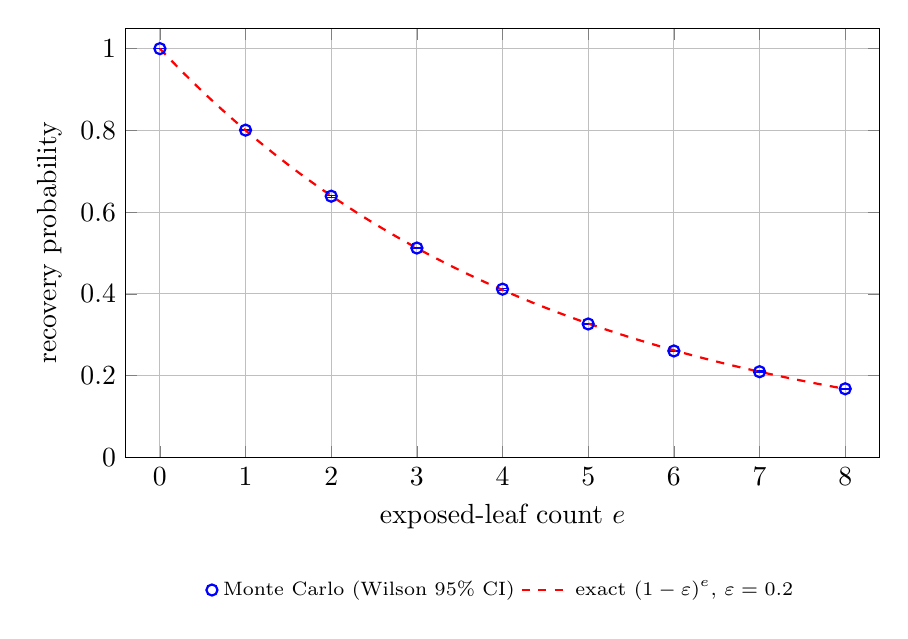
\begin{tikzpicture}
\begin{axis}[
  width=0.92\linewidth,
  height=0.58\linewidth,
  xmin=-0.4, xmax=8.4,
  ymin=0, ymax=1.05,
  xtick={0,1,2,3,4,5,6,7,8},
  grid=both,
  xlabel={exposed-leaf count \(e\)},
  ylabel={recovery probability},
  legend style={at={(0.5,-0.26)},anchor=north,draw=none,fill=none,font=\scriptsize,legend columns=2},
  legend cell align=left
]
\addplot+[only marks, mark=o, thick, error bars/.cd, y dir=both, y explicit]
  coordinates {
  (0,1.0) +- (0,0.0)
  (1,0.8007) +- (0,0.0018)
  (2,0.6391) +- (0,0.0021)
  (3,0.5123) +- (0,0.0022)
  (4,0.4117) +- (0,0.0022)
  (5,0.3265) +- (0,0.0021)
  (6,0.2605) +- (0,0.0019)
  (7,0.2097) +- (0,0.0018)
  (8,0.1679) +- (0,0.0016)
};
\addlegendentry{Monte Carlo (Wilson \(95\%\) CI)}
\addplot+[mark=none, thick, dashed, domain=0:8, samples=60] {0.8^x};
\addlegendentry{exact \((1-\varepsilon)^{e}\), \(\varepsilon=0.2\)}
\end{axis}
\end{tikzpicture}
\caption{Monte Carlo verification of the exact residual-leaf law
\eqref{eq:exact-residual-probability}: empirical all-survive frequency of
an \(e\)-leaf exposed set against the exact curve \((0.8)^{e}\).
Experiment E2 of the accompanying program.}
\label{fig:residual-law-mc}
\end{figure}

\paragraph*{MDS reliability}
The coded benchmark's recovery probability is the exact binomial cdf
\eqref{eq:mds-success-probability}.  We verify it at scale: for
\(\varepsilon=0.2\), \(\delta=0.1\), and \(n\in\{10^{3},10^{4},10^{5}\}\), we
simulate the erasure count and compare the empirical frequency of
\(\{E_{n}\le r_{\mathrm{MDS}}^{*}\}\) with the exact cdf.
Table~\ref{tab:mc-reliability} reports the results: at every scale the Monte
Carlo estimate matches the exact value within the confidence interval, and
both sit at the design target \(1-\delta=0.9\) (the small excess is the
integer-quantile granularity of \(r_{\mathrm{MDS}}^{*}\)).

\begin{table}[t]
\caption{Monte Carlo verification of the exact MDS reliability
\eqref{eq:mds-success-probability} at \(\varepsilon=0.2\), \(\delta=0.1\)
(\(6000\) trials per scale; Experiment E2, coded side).}
\label{tab:mc-reliability}
\centering
\begin{tabular}{@{}rrccc@{}}
\toprule
\(n\) & \(r_{\mathrm{MDS}}^{*}\) & MC reliability & Wilson \(95\%\) CI & exact \\
\midrule
\(10^{3}\) & \(216\)   & \(0.9070\) & \([0.8994,0.9141]\) & \(0.9031\) \\
\(10^{4}\) & \(2051\)  & \(0.9002\) & \([0.8923,0.9075]\) & \(0.9008\) \\
\(10^{5}\) & \(20162\) & \(0.9037\) & \([0.8959,0.9109]\) & \(0.9005\) \\
\bottomrule
\end{tabular}
\end{table}

These two verifications close the loop on the stochastic content of the
paper: the transparent side is governed by the exact survival power
\((1-\varepsilon)^{e}\), the coded side by the exact binomial quantile, and
both are confirmed by simulation to within Monte Carlo precision at the
scales used throughout.  The dispersion observable
\(\Delta_n=(r_{\mathrm{MDS}}^{*}-\varepsilon n)/\sqrt n\) of
\eqref{eq:dispersion-observable} is likewise consistent with its expansion
\eqref{eq:dispersion-expansion}: at \(\varepsilon=0.2\), \(\delta=0.1\)
the theoretical constant is
\(\sqrt{\varepsilon(1-\varepsilon)}\,\Phi^{-1}(1-\delta)\approx 0.5126\),
and the exact finite-\(n\) values fluctuate around it without visible
drift, with \(|\Delta_n-0.5126|\le0.031\) throughout the tested range
\(n\in[200,10^{5}]\) (Experiment E3).

\subsection{Validation of the Coded-Side Laws and the Large-Scale Overhead}
\label{subsec:numerical-coded-validation}

We next validate the coded-side results of Section~\ref{sec:coded-outer}
through three exactly computable observables, the numerical counterpart of
Theorems~\ref{thm:first-order-overhead-law}
and~\ref{thm:coded-strong-converse}.

\begin{remark}[Observable signatures implied by the coded-side laws]
\label{rem:coded-observables}
Fix \(\varepsilon\in(0,1)\), \(\delta\in(0,1/2)\), and
\(\gamma\in(0,\varepsilon)\).  Define
\begin{align}
  \mathcal R_n
  &:=
  \frac{\bigl(n-N^*(\varepsilon,\delta)\bigr)^+}
       {r_{\mathrm{MDS}}^*(n,\varepsilon,\delta)},
\label{eq:overhead-observable}\\
  \Delta_n
  &:=
  \frac{r_{\mathrm{MDS}}^*(n,\varepsilon,\delta)-\varepsilon n}
       {\sqrt n},
\label{eq:dispersion-observable}\\
  \mathcal E_n(\gamma)
  &:=
  -\frac{1}{n}\ln
  \Pr\!\bigl[
    \mathrm{Bin}(n,\varepsilon)
    \le
    \lfloor(\varepsilon-\gamma)n\rfloor
  \bigr].
\label{eq:exponent-observable}
\end{align}
Then, as \(n\to\infty\),
\begin{align}
  &\mathcal R_n
  =
  \frac{1}{\varepsilon}
  -
  \frac{\Phi^{-1}(1-\delta)\sqrt{1-\varepsilon}}
       {\varepsilon^{3/2}\sqrt n}
  +
  O\!\left(n^{-1}\right),
\label{eq:overhead-expansion}\\
  &\Delta_n
  =
  \sqrt{\varepsilon(1-\varepsilon)}\,\Phi^{-1}(1-\delta)
  +
  O\!\left(n^{-1/2}\right),
\label{eq:dispersion-expansion}\\
  &\lim_{n\to\infty}\mathcal E_n(\gamma)
  =
  D(\varepsilon-\gamma\|\varepsilon).
\label{eq:exponent-limit}
\end{align}
Indeed, substituting the second-order expansion
\eqref{eq:rstar-second-order} into \eqref{eq:overhead-observable} and
expanding the denominator gives \eqref{eq:overhead-expansion};
\eqref{eq:dispersion-expansion} is \eqref{eq:rstar-second-order} divided by
\(\sqrt n\); and \eqref{eq:exponent-limit} is Cram\'er's theorem applied to
the binomial lower tail, exactly as in the proof of
Theorem~\ref{thm:coded-strong-converse}.  Moreover, by
\eqref{eq:homogeneous-leaf-opt} and \eqref{eq:sigma-bar-one-packet}, and
under the standing Reed--Solomon alphabet condition of
Subsection~\ref{subsec:coded-benchmark-model}, \(\mathcal R_n\) coincides
with the normalized leaf-only/coded storage ratio of
Theorem~\ref{thm:first-order-overhead-law} up to the one-packet and
\((2^{c_B}-1)^{-1}\) slack of Theorem~\ref{thm:mds-near-optimality}.
\end{remark}

\paragraph*{Large-scale approach of the overhead ratio}
On a logarithmic grid up to \(n=10^{5}\), the exact ratio
\(\mathcal R_n\) remains strictly below the universal limit
\(1/\varepsilon\) for both erasure rates and approaches it monotonically.
Quantitatively, the relative overhead error
\(\mathrm{err}(n):=|1/\mathcal R_n-\varepsilon|/(1/\varepsilon)\)
decays approximately as \(n^{-1/2}\), as predicted by
\eqref{eq:overhead-expansion}, and reaches \(0.012\%\) at
\(\varepsilon=0.1\) and \(0.032\%\) at \(\varepsilon=0.2\) when
\(n=10^{5}\) (exact grid values from Experiment E1 of the accompanying
program).  The finite-\(n\) gap is thus governed by the \(\sqrt n\)
dispersion of the coded threshold.

\paragraph*{Strong-converse exponent}
Finally, the exponent observable \eqref{eq:exponent-observable} is evaluated
exactly at \(\varepsilon=0.3\) for the gaps
\(\gamma\in\{0.10,0.15,0.20\}\) of Table~\ref{tab:numerical-defaults}.  At
\(n=10^{3}\) (resp.\ \(10^{4}\)), \(\mathcal E_n(\gamma)\) equals
\(0.0289\), \(0.0639\), \(0.1205\) (resp.\ \(0.0262\), \(0.0615\),
\(0.1169\)), against the respective Cram\'er limits
\(D(\varepsilon-\gamma\|\varepsilon)=0.02573\), \(0.06106\), \(0.11632\):
the finite-\(n\) exponents approach the limit from above, confirming
\eqref{eq:exponent-limit}.  Per the regime
\eqref{eq:alphabet-growth-regime} of
Theorem~\ref{thm:coded-strong-converse}, this binomial lower-tail exponent
is the strong-converse exponent of the benchmark task itself whenever the
packet alphabet grows with \(c_B/n\to\nu\) and
\(\nu\ln 2>D(\varepsilon-\gamma\|\varepsilon)\)---at \(\gamma=0.10\), the
latter condition reads \(c_B/n>0.0371\) (Experiment E8).

\subsection{Single-Query Finite-Blocklength Comparison}
\label{subsec:numerical-single-query}

We first isolate the local structural kernel on a stylized single-query
family.  Fix a query \(q\) with \(\kappa_q\) base leaves and suppose its
canonical DAG contains \(M_{\mathrm{loc}}\) pairwise disjoint internal module
roots \(r_1,\ldots,r_{M_{\mathrm{loc}}}\) with
\(|\operatorname{Pdom}_q(r_j)|=s\), with no additional set-wise interception
beyond these designated modules.  Under this controlled construction, caching
\(m\) module roots removes exactly \(ms\) leaves from the exposed set.  The
finite-blocklength curves are
\begin{align}
  \widehat{\sigma}_{\mathrm{leaf}}^*
  (q,\varepsilon,\delta)
  &=
  \bigl(\kappa_q-N^*(\varepsilon,\delta)\bigr)^+,
\label{eq:numerical-local-leaf}\\
  \widehat{\sigma}_{\mathrm{sem,int}}^{\mathrm{loc}}(m)
  &=
  m\rho
  +
  \bigl(
    \kappa_q-ms-N^*(\varepsilon,\delta)
  \bigr)^{+},
\label{eq:numerical-local-sem}\\
  &\qquad
  0\le m\le M_{\mathrm{loc}},
\notag
\end{align}
together with the coded curve
\(\widehat{\bar{\sigma}}_{\mathrm{code}}^{\mathrm{loc}}
(q,\varepsilon,\delta)=r_{\mathrm{MDS}}^*(\kappa_q,\varepsilon,\delta)\).
The best semantic-aware local design is
\(\widehat{\sigma}_{\mathrm{sem,int}}^{*,\mathrm{loc}}
=\min_{0\le m\le M_{\mathrm{loc}}}
\widehat{\sigma}_{\mathrm{sem,int}}^{\mathrm{loc}}(m)\).

Three finite-blocklength effects follow directly from these closed
forms.  First, both
transparent curves are staircase functions of \((\varepsilon,\delta)\) through
the integer threshold \(N^{*}\).  Second, the coded benchmark is governed by a
binomial quantile rather than a hard survival threshold: it varies smoothly
and grows on the \(\varepsilon\kappa_q\)-scale, whereas the raw-premise
transparent law grows on the \(\kappa_q\)-scale.  Third, the semantic-aware
curve shifts the leaf-only curve downward by exactly \(m(s-\rho)\) whenever
the positive-part term in \eqref{eq:numerical-local-sem} is active, so the
single-query crossover occurs precisely at the structural threshold
\(\rho<s\) of Section~\ref{subsec:single-query-module-benchmark}.  Once
\(\kappa_q-ms\le N^{*}\), the module roots alone meet the reliability
target and the residual completion term disappears.
Experiment E5 evaluates the three curves on the grid
\(\varepsilon\in[0.02,0.30]\) with \(\kappa_q=40\), \(M_{\mathrm{loc}}=4\),
\(s=5\), \(\rho=0.4\), \(\delta=0.05\): once \(N^{*}=0\)
(\(\varepsilon>0.05\)), the leaf-only curve holds at \(40\) packets and the
semantic-aware curve at \(21.6\) packets---a downward shift of exactly
\(4(s-\rho)=18.4\)---while the coded benchmark rises smoothly from \(2\)
to \(17\) packets.

\subsection{Shared-Workload Ensemble with Reusable Modules}
\label{subsec:numerical-workload-family}

We now pass to a controlled workload family that matches the shared-module
framework of Section~\ref{sec:semantic-scenario} and the exact module-routing
regime of Definition~\ref{def:no-spurious-interception}.  The workload is
specified by five integers \((L,M,\mu,d,s,n_{\mathrm{priv}})\) satisfying
\(L\mu=Md\).  There are \(L\) queries; \(M\) pairwise disjoint shared leaf
groups \(H_1,\ldots,H_M\) of size \(s\); \(L\) pairwise disjoint private leaf
sets \(P_1,\ldots,P_L\) of size \(n_{\mathrm{priv}}\); and one internal
semantic-module root \(r_j\) above each shared group \(H_j\).  Each query
uses exactly \(\mu\) shared groups and one private group,
\begin{equation}
  D_\ell
  =
  P_\ell
  \cup
  \bigcup_{j\in\mathcal J_\ell}H_j,
  \qquad
  |\mathcal J_\ell|=\mu,
\label{eq:numerical-query-incidence}
\end{equation}
and each shared module is reused by exactly \(d\) queries.  The family is
constructed so that \(H_j\) is \(W\)-globally protected by \(r_j\) and the
exact module-routing condition holds: its query DAGs have depth two, with the
leaves of \(H_j\) routed through \(r_j\) and private leaves adjacent to the
query.  Under this construction every query has dependency size
\(\kappa_\ell=n_{\mathrm{priv}}+\mu s\), while the workload dependency union
has size
\(|D_{\mathrm{dep}}(W)|=Ln_{\mathrm{priv}}+Ms\).

\subsection{Joint-Criterion Results}
\label{subsec:numerical-joint-results}

Under the joint criterion the workload family yields clean closed forms.  If
a subset \(J\subseteq\{1,\ldots,M\}\) of shared roots is cached, every cached
root removes its whole protected group from the exposed-leaf union, so
\(|E_{\cup}(C_J)|=Ln_{\mathrm{priv}}+(M-|J|)s\).  Substituting into
\eqref{eq:numerical-sem-joint} and using symmetry in \(m:=|J|\),
\begin{equation}
  \begin{split}
    \widehat{\sigma}_{\mathrm{sem}}^{*,\mathrm{joint}}
    ( & W,\varepsilon,\delta)
    =
    \min_{0\le m\le M}
    \Bigl\{ m\rho \\
    & + \bigl( L n_{\mathrm{priv}} + (M-m)s - N^*(\varepsilon,\delta) \bigr)^+ \Bigr\}.
  \end{split}
\label{eq:numerical-joint-sem-opt}
\end{equation}
The joint leaf-only and coded curves are
\(\widehat{\sigma}_{\mathrm{leaf}}^{*,\mathrm{joint}}
=(Ln_{\mathrm{priv}}+Ms-N^{*})^{+}\) and
\(\widehat{\bar{\sigma}}_{\mathrm{code}}^{\mathrm{joint}}
=r_{\mathrm{MDS}}^{*}(Ln_{\mathrm{priv}}+Ms,\varepsilon,\delta)\).

\begin{figure}[t]
\centering
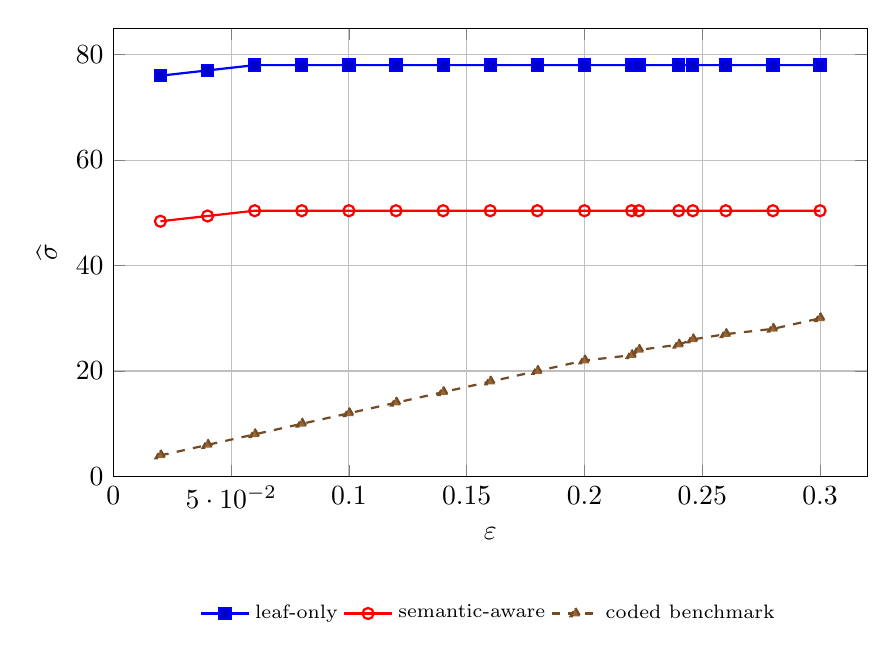
\begin{tikzpicture}
\begin{axis}[
  width=0.92\linewidth,
  height=0.6\linewidth,
  xmin=0, xmax=0.32,
  ymin=0, ymax=85,
  xtick={0,0.05,0.10,0.15,0.20,0.25,0.30},
  grid=both,
  xlabel={\(\varepsilon\)},
  ylabel={\(\widehat{\sigma}\)},
  legend style={at={(0.5,-0.26)},anchor=north,draw=none,fill=none,font=\scriptsize,legend columns=3},
  legend cell align=left
]
\addplot+[mark=square*, thick] coordinates {
  (0.02,76) (0.04,77) (0.06,78) (0.08,78) (0.10,78) (0.12,78)
  (0.14,78) (0.16,78) (0.18,78) (0.20,78) (0.22,78) (0.2231,78)
  (0.24,78) (0.246,78) (0.26,78) (0.28,78) (0.30,78)
};
\addlegendentry{leaf-only}
\addplot+[mark=o, thick] coordinates {
  (0.02,48.4) (0.04,49.4) (0.06,50.4) (0.08,50.4) (0.10,50.4)
  (0.12,50.4) (0.14,50.4) (0.16,50.4) (0.18,50.4) (0.20,50.4)
  (0.22,50.4) (0.2231,50.4) (0.24,50.4) (0.246,50.4) (0.26,50.4)
  (0.28,50.4) (0.30,50.4)
};
\addlegendentry{semantic-aware}
\addplot+[mark=triangle*, thick, dashed] coordinates {
  (0.02,4) (0.04,6) (0.06,8) (0.08,10) (0.10,12) (0.12,14)
  (0.14,16) (0.16,18) (0.18,20) (0.20,22) (0.22,23) (0.2231,24)
  (0.24,25) (0.246,26) (0.26,27) (0.28,28) (0.30,30)
};
\addlegendentry{coded benchmark}
\end{axis}
\end{tikzpicture}
\caption{Joint-criterion three-way comparison for the default
shared-workload ensemble (\(|D_{\mathrm{dep}}(W)|=78\), \(\delta=0.05\)).
The semantic-aware optimum caches all \(M=6\) shared roots, saving
\(27.6\) packets against the leaf-only baseline whenever the residual
completion term is active; the refined grid points \(0.2231\) and
\(0.246\) mark the coded-quantile jumps.  Experiment E6.}
\label{fig:workload-joint}
\end{figure}

Several conclusions follow from Fig.~\ref{fig:workload-joint}.  Whenever
the positive-part term in \eqref{eq:numerical-joint-sem-opt} remains
active, each cached module root trades a cost of \(\rho\) for the removal
of \(s\) exposed leaves, so the gain condition is again \(\rho<s\) and the
gain grows linearly with the total shared protected mass \(ms\).  As
\(n_{\mathrm{priv}}\) grows, the residual term dominates and the fractional
benefit of shared modules decreases.  And even when all \(M\) shared roots
are cached, the semantic-aware curve remains above the coded benchmark
whenever \(r_{\mathrm{MDS}}^{*}\) is substantially smaller than
\(M\rho+(Ln_{\mathrm{priv}}-N^{*})^{+}\): semantic reuse narrows the
transparent/coded gap but does not eliminate it.

\subsection{Maximal-Error Results}
\label{subsec:numerical-max-results}

Under the maximal-error criterion, the exact transparent costs are computed
from the binary programs just described.  The most informative special case is
the
\emph{fully shared} regime \(\mu=M\), \(d=L\), in which every query uses all
\(M\) shared modules, so \(D_\ell=P_\ell\cup H_1\cup\cdots\cup H_M\) and
\(\kappa_\ell=n_{\mathrm{priv}}+Ms\).  Then the exact maximal-error leaf-only
problem collapses to a one-dimensional search: if \(x\) shared leaves are
cached from the common pool, every query reduces its exposed count by \(x\),
and the remaining deficit is filled privately:
\begin{equation}
  \begin{split}
    \widehat{\sigma}_{\mathrm{leaf}}^{*,\max}( & W,\varepsilon,\delta)
    =
    \min_{0\le x\le Ms}
    \Bigl\{ x \\
    & + L\bigl( n_{\mathrm{priv}} + Ms - N^*(\varepsilon,\delta) - x \bigr)^+ \Bigr\}.
  \end{split}
\label{eq:numerical-max-leaf-fullshare}
\end{equation}
If in addition \(m\) shared module roots are cached, the common pool shrinks
to \((M-m)s\), giving the exact semantic-aware cost
\begin{equation}
  \begin{split}
    \widehat{\sigma}_{\mathrm{sem}}^{*,\max}
    ( & W,\varepsilon,\delta)
    = \min_{0\le m\le M}\Bigl\{ m\rho + \min_{0\le x\le (M-m)s} \Bigl[ x \\
    & + L\bigl( n_{\mathrm{priv}}+(M-m)s-N^* - x \bigr)^+ \Bigr] \Bigr\},
  \end{split}
\label{eq:numerical-max-sem-fullshare}
\end{equation}
The explicit coded benchmark is
\(\widehat{\bar{\sigma}}_{\mathrm{code}}^{\max}
=\min\{r_{\mathrm{MDS}}^{*}(Ln_{\mathrm{priv}}+Ms,\varepsilon,\delta),\,
L\,r_{\mathrm{MDS}}^{*}(n_{\mathrm{priv}}+Ms,\varepsilon,\delta)\}\).

\begin{figure}[t]
\centering
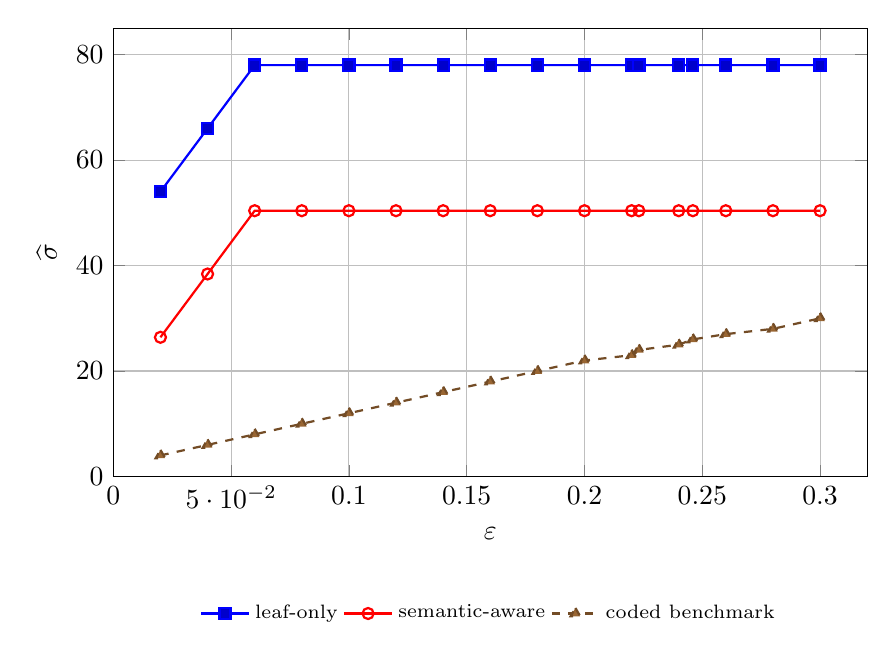
\begin{tikzpicture}
\begin{axis}[
  width=0.92\linewidth,
  height=0.6\linewidth,
  xmin=0, xmax=0.32,
  ymin=0, ymax=85,
  xtick={0,0.05,0.10,0.15,0.20,0.25,0.30},
  grid=both,
  xlabel={\(\varepsilon\)},
  ylabel={\(\widehat{\sigma}\)},
  legend style={at={(0.5,-0.26)},anchor=north,draw=none,fill=none,font=\scriptsize,legend columns=3},
  legend cell align=left
]
\addplot+[mark=square*, thick] coordinates {
  (0.02,54) (0.04,66) (0.06,78) (0.08,78) (0.10,78) (0.12,78)
  (0.14,78) (0.16,78) (0.18,78) (0.20,78) (0.22,78) (0.2231,78)
  (0.24,78) (0.246,78) (0.26,78) (0.28,78) (0.30,78)
};
\addlegendentry{leaf-only}
\addplot+[mark=o, thick] coordinates {
  (0.02,26.4) (0.04,38.4) (0.06,50.4) (0.08,50.4) (0.10,50.4)
  (0.12,50.4) (0.14,50.4) (0.16,50.4) (0.18,50.4) (0.20,50.4)
  (0.22,50.4) (0.2231,50.4) (0.24,50.4) (0.246,50.4) (0.26,50.4)
  (0.28,50.4) (0.30,50.4)
};
\addlegendentry{semantic-aware}
\addplot+[mark=triangle*, thick, dashed] coordinates {
  (0.02,4) (0.04,6) (0.06,8) (0.08,10) (0.10,12) (0.12,14)
  (0.14,16) (0.16,18) (0.18,20) (0.20,22) (0.22,23) (0.2231,24)
  (0.24,25) (0.246,26) (0.26,27) (0.28,28) (0.30,30)
};
\addlegendentry{coded benchmark}
\end{axis}
\end{tikzpicture}
\caption{Maximal-error three-way comparison in the fully shared regime
(\(\mu=M\), \(d=L\), \(\delta=0.05\)).  At low erasure rates, where
\(N^{*}\ge1\), the maximal-error transparent curves lie strictly below their
joint-criterion counterparts of Fig.~\ref{fig:workload-joint}, since
per-query exposed budgets can be met by query-private completion; the two
criteria coincide whenever \(N^{*}=0\).  Experiment E7.}
\label{fig:workload-max}
\end{figure}

These maximal-error curves, shown in Fig.~\ref{fig:workload-max},
sharpen the workload picture in two ways.
First, they separate the benefit of shared semantic compression from
ordinary shared raw-premise protection: a cached module root replaces an
entire protected group of \(s\) leaves at cost \(\rho\), so the decisive
tradeoff remains \(\rho<s\), exactly as the single-query theory predicts.
Second, the maximal-error criterion exposes the private component more
strongly: once the common shared deficit is removed, the remaining cost
scales like \(L(n_{\mathrm{priv}}-N^{*})^{+}\), which is purely
query-private and cannot be reduced further by shared modules.

\subsection*{Main Numerical Messages}
The numerical study closes the loop with
Sections~\ref{sec:single-query-kernel}--\ref{sec:coded-outer}: every
reported curve is either an exact evaluation of a theorem-level law or a
Monte Carlo estimate matching it within its Wilson confidence interval.
Four messages follow.

\paragraph*{1) The exact laws are confirmed by simulation at all reported
scales.}
The residual-leaf law \((1-\varepsilon)^{e}\) and the MDS binomial-quantile
reliability are matched by Monte Carlo estimates within Wilson \(95\%\)
confidence intervals, on the Datalog instance end to end, on the residual
family \(e=0,\ldots,8\), and on the coded benchmark up to \(n=10^{5}\).

\paragraph*{2) The single-query kernel is the correct local building block.}
At finite blocklength the transparent reliability law is governed by the
exposed-leaf count and exhibits the staircase structure induced by
\(N^{*}\); the local semantic gain appears exactly when a module root costs
less than the leaves it intercepts (\(\rho<s\)).

\paragraph*{3) Shared semantic modules materially reduce transparent
storage.}
Under the joint criterion, shared roots remove entire protected groups from
the exposed-leaf union, yielding the exact curve
\eqref{eq:numerical-joint-sem-opt}; the gain grows with the total protected
shared mass \(Ms\).

\paragraph*{4) The coded benchmark remains the outer reference, approached
at the universal rate.}
A residual coded advantage remains; the overhead ratio \(\mathcal R_n\)
approaches \(1/\varepsilon\) from below with relative error decaying as
\(n^{-1/2}\), reaching a few hundredths of one percent at \(n=10^{5}\).

The next section turns from finite-blocklength validation to conceptual
consequences, showing that the same exact laws admit natural
function-protection and maximal-recoverability readings within the present
stochastic-erasure model.

%%%%%%%%%%%%%%%%%%%%%%%%%%%%%%%%%%%%%%%%%%%%%%%%%%%%%%%%%%%%%%%%%%%%%%%%%%%%%%%%%
%%% Section VII
%%%%%%%%%%%%%%%%%%%%%%%%%%%%%%%%%%%%%%%%%%%%%%%%%%%%%%%%%%%%%%%%%%%%%%%%%%%%%%%%%
\section{Coding-Theoretic Counterparts}
\label{sec:coding-theoretic}

The numerical role of Section~\ref{sec:numerical} is now complete.  We turn
here to the conceptual coding-theoretic consequences of the exact
transparent-caching laws.  The point is not that the present model modifies
the classical worst-case FCC or MR frameworks; rather, it identifies a
structured stochastic-erasure regime in which constrained redundancy,
recoverability, and, in tractable cases, optimal design admit exact
closed-form laws.

In particular, the exact transparent laws admit a function-protection
reading and a derivation-level maximal-recoverability reading.  These are
statements within the present stochastic-erasure model; they are not claimed
as new worst-case theorems for the classical FCC or MR settings.

\subsection{An Exact Function-Protection Analogue under Stochastic Erasures}
\label{subsec:fcc-counterpart}

One way to read the present model is as a function-protection problem under
stochastic erasures.  The protected object is not the raw premise payload
itself, but the derivability of a query from that payload through a fixed
derivation structure.  In this sense, the paper studies a constrained form
of redundancy for function recovery rather than data recovery.

This viewpoint places the results next to the function-correcting-code
program, where redundancy is added so that a prescribed function value
survives worst-case symbol errors
\cite{lenz2023function,rajput2026function}.  The present paper studies the
corresponding question in a derivation-structured stochastic-erasure
setting rather than the classical worst-case one.  In that setting, the
protected object is the derivability event \(q\in\Cn(\cdot)\), and the
transparent-cache restriction turns the function-protection problem into
one that admits exact reliability laws and, in a tractable regime, exact
design laws.

Under the identification of Table~\ref{tab:fcc-mapping},
Definition~\ref{def:derivation-correcting} yields an exactly solvable
function-protection family in a stochastic-erasure regime.  Concretely,
the reliability law becomes the exposed-leaf formula
\((1-\varepsilon)^{|D_{\mathrm{exp}}|}\), feasibility becomes the explicit
threshold \(N^{*}(\varepsilon,\delta)\), and, under exact module routing,
the joint-criterion optimum is available in closed form.
Table~\ref{tab:regime-contrast} summarizes this change of viewpoint from
the worst-case FCC setting to the present stochastic-erasure setting.

\begin{table}[t]
\caption{Object-level correspondence between function-correcting codes
and the present model.}
\label{tab:fcc-mapping}
\centering\footnotesize
\begin{tabularx}{\columnwidth}{@{}LL@{}}
\toprule
FCC~\cite{lenz2023function,rajput2026function} & Present model \\
\midrule
data vector \(u\in\mathbb F_q^{k}\), systematic part exposed to errors &
premise base \(B\), systematic logical content exposed to erasures \\
function \(f\colon\mathbb F_q^{k}\to\mathrm{Im}(f)\), fixed a priori &
derivability map \(B\mapsto\Cn(B)\), induced by the derivation rules;
each query \(q\) is the Boolean function \(\mathbf 1[q\in\Cn(B)]\) \\
choice of \(f\) fixes the instance & choice of derivation rules fixes
the instance \\
redundancy part: \(r\) appended symbols, unconstrained & cache
\(S\subseteq\Cn(B)\): appended consequences, semantically constrained \\
decoder outputs \(f(u)\) despite any \(t\) worst-case symbol errors &
query \(q\) answered despite i.i.d.\ premise erasures \\
optimal redundancy \(r_{f}(k,t)\) & optimal redundancy
\(\sigma_{\mathrm{dc}}^{*}(W,\varepsilon,\delta)\)
(Definition~\ref{def:derivation-correcting}) \\
\bottomrule
\end{tabularx}
\end{table}

\begin{definition}[Derivation-correcting storage]
\label{def:derivation-correcting}
Fix a workload \(W\subseteq\mathcal Q\), an erasure rate
\(\varepsilon\in(0,1)\), and a tolerance \(\delta\in(0,1)\).  A finite
answer-excluding cache \(S\subseteq\Cn(B)\setminus W\) is
\emph{\((W,\varepsilon,\delta)\)-derivation-correcting} if the joint
criterion \eqref{eq:model-joint-criterion} holds, and the \emph{optimal
redundancy} \(\sigma_{\mathrm{dc}}^{*}(W,\varepsilon,\delta)\) is the
minimum storage cost of such a cache.  The exclusion of \(W\) is the
standing convention of Section~\ref{sec:model}: storing the requested
answers themselves is direct result caching, not structural redundancy.
Thus
\[
  \sigma_{\mathrm{dc}}^{*}(W,\varepsilon,\delta)
  =
  \sigma_{\mathrm{sem}}^{*,\mathrm{joint}}(W,\varepsilon,\delta).
\]
\end{definition}

Definition~\ref{def:derivation-correcting} is the analogue of the
\((f,t)\)-FCC problem obtained by passing to the stochastic-erasure
regime.  Under this substitution, the
worst-case sandwich is replaced by an exact exposed-leaf characterization;
within the exact module-routing regime, the optimal redundancy itself is
evaluated in closed form.

\begin{corollary}[Exact erasure-regime redundancy laws]
\label{cor:erasure-regime-redundancy}
For the derivability function family, the reliability of any candidate
cache is the closed form \((1-\varepsilon)^{|D_{\mathrm{exp}}(q,S)|}\) of
Theorem~\ref{thm:exact-residual-law}; feasibility is characterized exactly
by the integer threshold \(N^{*}(\varepsilon,\delta)\)
(Corollaries~\ref{cor:exact-reliability-threshold}
and~\ref{cor:workload-thresholds}); under the hypotheses of
Theorem~\ref{thm:shared-module-exact-optimality}, including exact module
routing and homogeneous leaf costs, the shared-module cache attains the
closed-form joint-criterion optimum over all answer-excluding transparent
caches; and the benchmark-relative overhead has the first-order limits
\(1/\varepsilon\) and \(\rho/(s\varepsilon)\) in the leaf-only and
saturated shared regimes, respectively
(Theorem~\ref{thm:first-order-overhead-law} and
Remark~\ref{rem:asymptotic-overhead-alpha}).
\end{corollary}

\begin{proof}
Each clause is a restatement of the cited result in the notation of
Definition~\ref{def:derivation-correcting}.
\end{proof}

Under the identification of Table~\ref{tab:fcc-mapping},
Definition~\ref{def:derivation-correcting} becomes an exactly solvable
function-protection family in a stochastic-erasure regime.  The point is
not that the present model subsumes the classical worst-case FCC problem.
Rather, it isolates a structured family for which the function-recovery
question admits exact reliability laws and, under exact module routing, a
closed-form optimal design.  In that precise sense, the paper contributes a
coding-theoretic consequence of the transparent-caching theory, not merely
an after-the-fact analogy.
Table~\ref{tab:regime-contrast} summarizes what the solution adds to the
correspondence itself: the general sandwich characterization is replaced by
an exact reliability law, the representative-vector equality condition by
the checkable exact module-routing regime, and the combinatorial evaluation
of \(N(D)\) by the explicit threshold \(N^{*}(\varepsilon,\delta)\).
The stylized workload ensemble of
Subsections~\ref{subsec:numerical-workload-family}
and~\ref{subsec:numerical-joint-results} is such a solved instance in
concrete form: its function family---shared-module derivability with
depth-two witnesses---has exact redundancy curves, saving \(27.6\) of
\(78\) packets against the leaf-only baseline.

\begin{table}[t]
\caption{Function protection in the worst-case and stochastic-erasure
regimes.}
\label{tab:regime-contrast}
\centering\footnotesize
\begin{tabularx}{\columnwidth}{@{}p{.19\columnwidth}LL@{}}
\toprule
 & FCC~\cite{lenz2023function,rajput2026function} & This paper \\
\midrule
Error model & \(t\) worst-case symbol errors & i.i.d.\ premise erasures,
rate \(\varepsilon\) \\
Protected object & function value \(f(u)\) & derivability
\(q\in\Cn(\cdot)\) \\
Redundancy law & DRM--FDM sandwich; exact or nearly tight laws in
special structured regimes & exact reliability law; staircase feasibility
threshold \(N^{*}\) \\
Evaluation & combinatorial \(N(D)\) optimization; special-function closed
forms & closed-form threshold \(N^{*}\); residual selection NP-complete
already at depth two \\
\bottomrule
\end{tabularx}
\end{table}

Two further consistency points are worth noting.  The observation
of~\cite{rajput2026function} that perfect and MDS codes provide no
additional function-value protection is consistent with the benchmark role
that MDS codes play here (Theorem~\ref{thm:mds-near-optimality}): in both
regimes, code optimality and function protection are distinct notions.
And the hardness clause of Proposition~\ref{prop:module-selection-np-hard}
mirrors the combinatorial difficulty of evaluating \(N(D)\) for general
functions, notwithstanding the exact or nearly tight special-function laws
of~\cite{zhang2025optimal,ly2025redundancy}.

The correspondence is not only object-level but proof-level.  In the FCC
framework, protection is a separation requirement on a demand
graph---representations of function-differing data pairs must be
separated---and the optimal redundancy is the combinatorial quantity
\(N(D)\).  In the erasure regime, protection is an interception
requirement on the derivation DAG, and the redundancy problem takes a
blocking-set form.

\begin{proposition}[Worst-case specialization and the blocking-set form]
\label{prop:worst-case-blocking}
Fix a non-base query \(q\in\mathcal Q\setminus B\) and an answer-excluding
cache \(S\subseteq\Cn(B)\setminus\{q\}\).  The following are equivalent:
\begin{enumerate}[label=(\roman*)]
\item \(q\) is recovered under every pattern of at most \(t\) erased
premises, for a prescribed \(t\ge 1\);
\item \(q\) is recovered under every erasure pattern whatsoever;
\item \(D_{\mathrm{exp}}(q,S)=\varnothing\);
\item \(q\in\Cn(S)\).
\end{enumerate}
Hence the minimum-cost answer-excluding cache protecting \(q\) against
worst-case premise erasures is exactly the minimum-cost complete blocking
set of the canonical DAG \(G_q\): a vertex set not containing \(q\) and
meeting every directed path from a base leaf to \(q\).
\end{proposition}

\begin{proof}
(iii)\(\Leftrightarrow\)(iv) is
Theorem~\ref{thm:exact-residual-law}\eqref{eq:exact-residual-event} with
\(\widetilde B=\varnothing\).  (ii)\(\Rightarrow\)(i) is trivial.
(i)\(\Rightarrow\)(iii): if \(D_{\mathrm{exp}}(q,S)\neq\varnothing\),
erasing a single exposed leaf---a pattern of weight \(1\le t\)---causes
failure by \eqref{eq:exact-residual-event}.
(iii)\(\Rightarrow\)(ii): if \(D_{\mathrm{exp}}(q,S)=\varnothing\), the
same equivalence yields recovery for every \(\widetilde B\), including
\(\widetilde B=\varnothing\).
\end{proof}

\begin{corollary}[Blocking-set equivalence and hardness]
\label{cor:blocking-hardness}
Answer-excluding worst-case redundancy minimization for
derivation-correcting storage is the minimum-cost complete blocking-set
problem on derivation DAGs.
Allowing a residual budget \(|D_{\mathrm{exp}}(q,S)|\le N^{*}\) yields the
partial blocking-set problem \eqref{eq:exact-single-query-opt}: deciding
the cheapest way to leave at most \(N^{*}\) leaves exposed is NP-complete
already at depth two (Proposition~\ref{prop:module-selection-np-hard}),
and Remark~\ref{rem:tractability-boundary} shows that this tractability
boundary is sharp.
\end{corollary}

\begin{proof}
The equivalence is Proposition~\ref{prop:worst-case-blocking} together
with the cost model of Section~\ref{sec:model}; the hardness clause is
Proposition~\ref{prop:module-selection-np-hard}.
\end{proof}

\begin{remark}[\(N^{*}\) as the worst-case premium]
\label{rem:nstar-premium}
Comparing Proposition~\ref{prop:worst-case-blocking} with the stochastic
reliability criterion \(|D_{\mathrm{exp}}(q,S)|\le
N^{*}(\varepsilon,\delta)\) gives the threshold a second reading: the
\((\varepsilon,\delta)\)-stochastic requirement tolerates exactly
\(N^{*}\) exposed leaves that worst-case (reliability-one) protection
would forbid.  The staircase threshold is thus precisely the premium, in
unprotected leaves, that the worst-case requirement charges over the
stochastic one---and relaxing to the stochastic regime is what makes
graded, closed-form protection possible at all.
\end{remark}

\begin{remark}[Proof-level correspondence]
\label{rem:proof-objects}
The FCC demand graph and the canonical derivation DAG play analogous roles:
both encode which perturbations threaten the protected function.  The key
difference is that, in the present stochastic-erasure regime, partial
protection has an exact value, namely
\((1-\varepsilon)^{|D_{\mathrm{exp}}|}\), rather than only a worst-case
combinatorial interpretation.
\end{remark}

The role of the canonical regime is therefore methodological: it isolates a
structured stochastic-erasure family in which the coding-theoretic
analogue is exact, after Section~\ref{sec:numerical} has already shown that
the same family is quantitatively faithful at finite blocklength.
The point is not to modify the classical worst-case FCC
or MR models, but to identify a different regime in which constrained
redundancy, recoverability, and optimal design admit closed-form laws.

\subsection{A Derivation-Level Distributional Analogue of Maximal Recoverability}
\label{subsec:semantic-mr}

The present theory also has a natural maximal-recoverability reading.
Classical maximally recoverable codes are designed so that every erasure
pattern correctable in principle under the imposed locality structure is in
fact corrected.  In our setting, the analogue is derivation-level rather
than symbol-level: for a fixed cache and erasure realization, every query
that remains derivable from the surviving premises and the cache is
recovered.

What the present model adds is exact distributional quantification of this
maximality principle under i.i.d.\ erasures.  Instead of reasoning
pattern-by-pattern, the recovery probability collapses to a closed form,
namely the exposed-leaf laws of
Sections~\ref{sec:single-query-kernel} and
\ref{sec:semantic-scenario}.  Thus the link with maximal recoverability is
not only philosophical; it is operational, in the sense that the analogue
of ``all recoverable objects are recovered'' admits an exact stochastic law.

\begin{proposition}[Semantic maximal recoverability]
\label{prop:semantic-mr}
Fix any realization \((\widetilde B,S)\).  The set of workload queries
recovered by the transparent system is exactly
\(\{q\in W:\ q\in\Cn(\widetilde B\cup S)\}\); that is, the system recovers
every query that is recoverable in principle from the surviving material.
\end{proposition}

\begin{proof}
Immediate from the joint criterion \eqref{eq:model-joint-criterion}: each
query \(q_\ell\in W\) is answered exactly when
\(q_\ell\in\Cn(\widetilde B\cup S)\), so no query derivable from the
surviving premises and the cache is left unrecovered, and no other query
is.
\end{proof}

Proposition~\ref{prop:semantic-mr} is the definitional half of maximal
recoverability; Theorem~\ref{thm:exact-residual-law} supplies the
distributional half.  For every cache \(S\) and erasure rate
\(\varepsilon\), the reliability of the semantically maximally recoverable
system is evaluated in closed form,
\((1-\varepsilon)^{|D_{\mathrm{exp}}(q,S)|}\), rather than certified
pattern by pattern.  In the exact symbol-level MR theory
of~\cite{martinez2026maximally}, evaluating the probability of
correctability would require summing over the correctable-pattern family,
which grows exponentially with the block length; practical studies therefore
use Monte Carlo evaluation~\cite{kadekodi2023wide}.  For
derivation-structured content the same question collapses to a single
exponent---the exposed residual-leaf count---because the recovered event is
monotone in the surviving derivation structure.  The workload-level theory
lifts this evaluation to the whole system.

\begin{proposition}[Exact workload-level quantification]
\label{prop:workload-mr-quantification}
Let the cache satisfy the transparent semantics of
Section~\ref{sec:model}.  Then, for every erasure rate \(\varepsilon\),
the joint reliability of the semantically maximally recoverable system is
given exactly by the workload reliability laws of
Theorem~\ref{thm:workload-rigidity}; and, under the hypotheses of
Theorem~\ref{thm:shared-module-exact-optimality}, including exact module
routing and homogeneous leaf costs, the minimum-cost joint-criterion cache
meeting any prescribed reliability is characterized exactly by that
theorem.
\end{proposition}

\begin{proof}
Both clauses are restatements of the cited theorems, whose hypotheses
are precisely the transparent semantics and, for the second clause, the
exact module-routing regime.
\end{proof}

Proposition~\ref{prop:workload-mr-quantification} identifies an exact
distributional analogue of the maximal-recoverability principle for
derivation-structured content: both reliability and, under exact module
routing, minimum-cost design are available in closed form within the
present stochastic-erasure model.  This is narrower than a symbol-level MR
claim, but stronger than a loose analogy, because it is backed directly by
the transparent recovery theorems proved earlier in the paper.

\begin{table}[t]
\caption{Symbol-level maximal recoverability and its derivation-level
distributional counterpart.}
\label{tab:mr-contrast}
\centering\footnotesize
\begin{tabularx}{\columnwidth}{@{}p{.19\columnwidth}LL@{}}
\toprule
 & Symbol-level MR~\cite{martinez2026maximally} & Semantic MR (this
paper) \\
\midrule
Definition of maximality & correct every erasure pattern correctable in
principle under the locality constraints & recover every query derivable
from the surviving material
(Proposition~\ref{prop:semantic-mr}) \\
Evaluation object & symbol strings with local repair sets & derivation
DAGs over premise bases \\
Probabilistic evaluation & exact law not pursued; empirical Monte Carlo in
practice & closed form \((1-\varepsilon)^{|D_{\mathrm{exp}}|}\)
(Theorem~\ref{thm:exact-residual-law}) \\
Optimal-design condition & code constructions over finite fields;
field-size bounds & joint-criterion shared-module cache; exact
module-routing regime
(Theorem~\ref{thm:shared-module-exact-optimality}) \\
Regime & worst case & stochastic erasures \\
\bottomrule
\end{tabularx}
\end{table}

\begin{remark}[Modules as locality-like repair objects]
\label{rem:module-as-lrc}
A shared module root \(r_j\) together with its protected leaf group
\(H_j\) of size \(s\) plays a locality-like role: one stored object of
normalized cost \(\rho=c_I/c_B\) protects all \(s\) leaves in the group, so
the effective protection cost is \(\rho/s\) per leaf.  This is strictly
cheaper than caching leaves individually exactly when \(\rho<s\), the
strict-gain threshold of Section~\ref{sec:semantic-scenario}.  The analogy
should be read at the level of protected functionality rather than symbol
reconstruction: the module restores the leaves' contribution to the query,
not their payload values.  What blocking buys is graded reliability:
complete blocking gives worst-case reliability one
(Proposition~\ref{prop:worst-case-blocking}), and partial blocking has the
exact stochastic value \((1-\varepsilon)^{|D_{\mathrm{exp}}|}\)
(Theorem~\ref{thm:exact-residual-law}).
\end{remark}

\subsection{Coding-Theoretic Significance and Two Open Programs}
\label{subsec:open-programs}

The main lesson of this section is that transparent recovery under premise
erasures defines a nontrivial coding-theoretic family.  Its exact laws can
be read as structured stochastic-erasure analogues of function protection
and maximal recoverability, and the same structural restrictions that make
the model semantically meaningful also make it analytically tractable.
The open programs below ask how far these exact laws can be pushed beyond
the present derivation-structured regime.

\paragraph*{Function-correcting storage beyond derivability}
A stochastic-erasure FCC theory beyond derivability would have to replace
the worst-case irregular-distance quantity \(N(D)\) by reliability
thresholds induced by the erasure law.  The derivability family analyzed here
provides a concrete solved instance;
locally bounded and linear function families
\cite{premlal2025function,verma2026function} are natural next candidates.

\paragraph*{Exact reliability laws for maximally recoverable codes}
In regimes where the correctable-pattern family is characterized exactly,
as in~\cite{martinez2026maximally}, the probability of correctability under
i.i.d.\ erasures is a well-defined combinatorial sum over that family.
Evaluating such sums in closed form---the residual-leaf law is the solved
instance for derivation-structured content---would convert worst-case
maximal recoverability into exact distributional reliability laws.

%%%%%%%%%%%%%%%%%%%%%%%%%%%%%%%%%%%%%%%%%%%%%%%%%%%%%%%%%%%%%%%%%%%%%%%%%%%%%%%%%
%%% Section VIII
%%%%%%%%%%%%%%%%%%%%%%%%%%%%%%%%%%%%%%%%%%%%%%%%%%%%%%%%%%%%%%%%%%%%%%%%%%%%%%%%%
\section{Discussion and Conclusion}
\label{sec:discussion}

\paragraph{Why the Strong Assumptions Are Still Useful}
\label{para:discussion-strong-assumption}
Assumptions~\ref{assump:det-local} and~\ref{assump:hereditary-dag}
deliberately restrict the model to an exact canonical regime; they are not
meant to describe arbitrary reasoning systems.  Their value is that this
regime admits a theorem-level characterization of proof-valid recovery:
recovery succeeds if and only if no erased base leaf retains a cache-free
path to the target.  The exact kernel is then deployed inside the broader
workload-level story of reusable semantic modules
\cite{brachman2004knowledge,darwiche2002knowledge}.  Without such a
canonical regime, the connection between deductive structure and
erasure-channel theory would remain heuristic rather than theorem-level.

\paragraph{Relaxing Deterministic Local Semantics}
\label{para:discussion-nondeterminism}
The relaxation toward multiple admissible parent tuples is carried out in
Subsection~\ref{subsec:envelope-nonunique} and
Appendix~\ref{app:envelope}.  Under the AND--OR local semantics of
Assumption~\ref{assump:and-or-local}, the exact residual law survives as
the envelope law of Theorem~\ref{thm:envelope-rigidity}: recovery is a
monotone DNF in the survival indicators, sandwiched between the best
single witness and a union bound.  The canonical theory persists on both
sides.  Single-witness-certified caches remain reliable at no additional
cost (Corollary~\ref{cor:envelope-certified-threshold}), and converses
lose only an additive slack \(\Delta_{\mathcal G}\le\Lambda_q/\varepsilon\),
which leaves every first-order law unchanged whenever
\(\Lambda_q=o(\kappa_q^{\min})\)
(Corollary~\ref{cor:envelope-relaxation-cost}).
What remains open is the
algorithmic side: selecting module roots that postdominate uniformly over
the whole candidate family \(\mathcal G_S(q,B)\).

\paragraph{Partial Transparency and Hybrid Caches}
\label{para:discussion-partial}
The main development treats transparency as an all-or-nothing architectural
constraint.  Caches that split the budget between transparent leaves and
coded parity packets would interpolate between the two architectures
studied here and trace a storage--interpretability frontier; a general
hybrid theory with heterogeneous costs remains open.

\paragraph{Position within information theory}
The paper should be read as a study of constrained redundancy under
erasures.  Its exact laws are derived in a canonical derivation regime, but
their content is information-theoretic: they quantify how much reliability
is lost when redundancy is restricted to semantically admissible objects,
and how much of that loss can be recovered by sharing internal structure.
Section~\ref{sec:numerical} validates these claims at finite blocklength
and workload scale, while Section~\ref{sec:coding-theoretic} shows that
the same laws admit exact function-protection and
maximal-recoverability readings within a structured stochastic-erasure
model.  In this sense, the logical apparatus is not external packaging; it
is the structural mechanism that exposes a new solvable family of
redundancy problems.

\paragraph{Limitations}
\label{para:discussion-limitations}
Three boundaries of the present results should be kept in view.  First, the
coded side of the paper analyzes the explicit payload-recovery benchmark of
Definition~\ref{def:coded-benchmark-task}, not the true unrestricted coded
optimum.  The benchmark is essentially tight as a benchmark
(Remark~\ref{rem:benchmark-tightness}), but a coded cache may in principle
answer the workload without reconstructing every dependent payload.  Since
the true coded optimum can only lie lower, the benchmark-relative overhead
laws lower-bound the true transparency price; certifying such floors at the
level of the true coded optimum requires converses that depend on the
information content of the query outputs.  The quantitative coded-side
laws are also tied to the homogeneous packet model and its alphabet-growth
conventions of Section~\ref{sec:coded-outer}.  Second, exact transparent
optima are established only in structured regimes---exact module routing
and the unique-path case---while optimal cache selection in general DAGs is
NP-complete (Proposition~\ref{prop:module-selection-np-hard}); outside
these islands, the practical content of the theory is the certified
sufficient condition of
Theorem~\ref{thm:workload-shared-module-gain}.  Third, the numerical
evidence is mechanism-level: it is obtained on controlled synthetic
ensembles and one hand-checkable Datalog instance, and it demonstrates
agreement with the exact laws rather than performance on real reasoning
workloads.  Validation on workloads derived from practical deductive
systems, online variants with sequential query arrivals, and extensions to
correlated or adversarial erasures remain future work.

\paragraph*{Conclusion}
This paper develops a two-level theory of transparent recovery under premise
erasures.  At the exact local level, proof-valid recovery is governed by
canonical derivation structure and exposed dependencies: the query-local
rigidity theorem reduces arbitrary caches to their projection on the target
DAG, and the exact residual-leaf law yields the closed-form threshold
\(N^*(\varepsilon,\delta)\) for transparent storage.  At the systems level,
once transparency is mandatory, semantic structure is not merely a burden:
caching shared internal consequences as semantic modules strictly reduces the
required explicit storage, with an exact and constructive gain that in the
saturated regime depends only on the postdominated mass \(s\) and the module
cost \(\rho\) through the overhead law \(\alpha=\rho/(s\varepsilon)\).
Against the explicit coded outer benchmark, the leaf-only transparent
endpoint carries the universal first-order factor \(1/\varepsilon\),
which the saturated shared-module regime replaces by the module-scaled
law \(\alpha=\rho/(s\varepsilon)\) stated above.  Section~\ref{sec:numerical} confirms these laws
quantitatively through end-to-end Datalog verification, Monte Carlo checks,
and finite-blocklength workload curves; Section~\ref{sec:coding-theoretic}
shows that the same theorems also yield exact stochastic-erasure
counterparts of function protection and maximal recoverability for
derivation-structured content.  Semantic transparency thus creates both a
\emph{cost} relative to unrestricted coding and a \emph{gain} relative to
structure-oblivious transparent storage---a dual message that grounds a
broader theory of semantics-aware information storage and transmission.

\appendices

\counterwithin{definition}{section}
\counterwithin{axiom}{section}
\counterwithin{assumption}{section}
\counterwithin{theorem}{section}
\counterwithin{lemma}{section}
\counterwithin{proposition}{section}
\counterwithin{corollary}{section}
\counterwithin{remark}{section}
\counterwithin{example}{section}
\counterwithin{equation}{section}
%%%%%%%%%%%%%%%%%%%%%%%%%%%%%%%%%%%%%%%%%%%%%%%%%%%%%%%%%%%%%%%%%%%%%%%%%%%%%%%%
%%% Appendix A
%%%%%%%%%%%%%%%%%%%%%%%%%%%%%%%%%%%%%%%%%%%%%%%%%%%%%%%%%%%%%%%%%%%%%%%%%%%%%%%%
\section{Envelope-Law Consequences}
\label{app:envelope}

This appendix collects the consequences of the envelope law
(Theorem~\ref{thm:envelope-rigidity}) that are used outside the single-query
kernel: robust certification of single-witness designs and the quantified
converse slack.  The notation of
Subsection~\ref{subsec:envelope-nonunique} is retained throughout.

\begin{corollary}[Robust certification: single-witness designs remain valid]
\label{cor:envelope-certified-threshold}
Under Assumption~\ref{assump:and-or-local}, if there exists
\(G_0\in\mathcal G_S(q,B)\) with \(e_{G_0}(q,S)\le N^*(\varepsilon,\delta)\),
then \(S\) is \((\varepsilon,\delta)\)-reliable for \(q\).  It thus suffices
to verify the bound on a single \(B\)-grounded witness, for instance the
canonical DAG of the unique-tuple sub-model.
\end{corollary}

\begin{proof}
By definition \(e_*(q,S)\le e_{G_0}(q,S)\le N^*(\varepsilon,\delta)\), so the
lower bound in \eqref{eq:envelope-probability} gives
\(\Pr_{\varepsilon}[q\in\Cn(\widetilde B\cup S)]
\ge(1-\varepsilon)^{e_*(q,S)}
\ge(1-\varepsilon)^{N^*(\varepsilon,\delta)}\ge1-\delta\).
\end{proof}

Consequently, every achievable cache of
Sections~\ref{sec:single-query-kernel} and~\ref{sec:semantic-scenario} was
certified by exhibiting one DAG with exposed-leaf count at most
\(N^*(\varepsilon,\delta)\), and therefore certifies reliability verbatim,
at unchanged cost, under the full AND--OR semantics.

\begin{corollary}[Quantified relaxation cost: the converse slack]
\label{cor:envelope-relaxation-cost}
Under Assumption~\ref{assump:and-or-local}, define the ambiguity budget, the
ambiguity slack, and the inflated threshold by
\begin{align}
  \Lambda_q
  &:=
  \sum_{v\in\mathcal V_{\mathrm{rel}}(B)\setminus B}\ln(1+r_v),\nonumber\\
  \Delta_{\mathcal G}
  &:=
  \frac{\Lambda_q}{\ln\!\bigl(1/(1-\varepsilon)\bigr)},
  \nonumber\\
  N^+_{\mathcal G}(\varepsilon,\delta)
  &:=
  \left\lfloor
    \frac{
      \ln\!\bigl(1/(1-\delta)\bigr)+\Lambda_q
    }{
      \ln\!\bigl(1/(1-\varepsilon)\bigr)
    }
  \right\rfloor .
\label{eq:envelope-N-plus}
\end{align}
If \(S\) is \((\varepsilon,\delta)\)-reliable for \(q\), then
\begin{equation}
  e_*(q,S)
  \le
  N^+_{\mathcal G}(\varepsilon,\delta)
  \le
  N^*(\varepsilon,\delta)+\Delta_{\mathcal G}+1.
\label{eq:envelope-converse}
\end{equation}
Hence every converse of Sections~\ref{sec:single-query-kernel} and
\ref{sec:semantic-scenario} stated as a lower bound on storage remains valid
in the relaxed model after replacing \(N^*\) by \(N^+_{\mathcal G}\).
Explicitly, for the homogeneous leaf-only class, with
\(\kappa_q^{\min}:=\min_{G\in\mathcal G(q,B)}|V_0(G)|\),
\begin{equation}
  \begin{aligned}
    & \bigl(\kappa_q^{\min}-N^+_{\mathcal G}(\varepsilon,\delta)\bigr)^+ c_B \\
    \le &\sigma_{\mathrm{leaf,AO}}^{*}(q,\varepsilon,\delta) \\
    \le &\bigl(\kappa_q^{\min}-N^*(\varepsilon,\delta)\bigr)^+ c_B,
  \end{aligned}
\label{eq:envelope-leaf-sandwich}
\end{equation}
where \(\sigma_{\mathrm{leaf,AO}}^{*}\) is the leaf-only optimum under the
AND--OR semantics; the two sides differ by at most
\((\Delta_{\mathcal G}+1)c_B\).  Finally,
\begin{equation}
  \Delta_{\mathcal G}
  \le
  \frac{\Lambda_q}{\varepsilon},
\label{eq:envelope-slack-bound}
\end{equation}
so the slack is logarithmic in the per-vertex derivation multiplicities and
only ambiguous vertices contribute genuine derivation diversity.
\end{corollary}

\begin{proof}
By \eqref{eq:candidate-count-bound},
\(|\mathcal G_S(q,B)|\le e^{\Lambda_q}\).  Reliability and the upper bound in
\eqref{eq:envelope-probability} give
\(1-\delta\le\Pr_{\varepsilon}[q\in\Cn(\widetilde B\cup S)]
\le e^{\Lambda_q}(1-\varepsilon)^{e_*(q,S)}\),
and solving for the integer \(e_*(q,S)\) yields
\eqref{eq:envelope-converse}; the comparison with \(N^*(\varepsilon,\delta)\)
is immediate from \eqref{eq:model-N-star}.  For
\eqref{eq:envelope-leaf-sandwich}, let \(S\subseteq B\).  Then every
\(S\)-relative candidate is \(B\)-grounded, and a path from a base leaf is
cache-free if and only if its first vertex is not cached, so
\(e_G(q,S)=|V_0(G)\setminus S|=\kappa_G-|S\cap V_0(G)|\) with
\(\kappa_G:=|V_0(G)|\).  The upper side of
\eqref{eq:envelope-leaf-sandwich} follows by caching any
\((\kappa_q^{\min}-N^*)^+\) leaves of a \(B\)-grounded witness attaining
\(\kappa_q^{\min}\) and applying
Corollary~\ref{cor:envelope-certified-threshold}.  For the lower side,
reliability forces \(e_*(q,S)\le N^+_{\mathcal G}\), i.e.\
\(|S\cap V_0(G)|\ge\kappa_G-N^+_{\mathcal G}\) for some \(G\), hence
\(|S|\ge(\kappa_q^{\min}-N^+_{\mathcal G})^+\).
Finally \eqref{eq:envelope-slack-bound} uses
\(\ln(1/(1-\varepsilon))\ge\varepsilon\).
\end{proof}

%%%%%%%%%%%%%%%%%%%%%%%%%%%%%%%%%%%%%%%%%%%%%%%%%%%%%%%%%%%%%%%%%%%%%%%%%%%%
%%%%%% Reproducibility Statement
%%%%%%%%%%%%%%%%%%%%%%%%%%%%%%%%%%%%%%%%%%%%%%%%%%%%%%%%%%%%%%%%%%%%%%%%%%%%
\section*{Reproducibility Statement}
All numerical values reported in Section~\ref{sec:numerical} are generated from
explicit formulas stated in the paper together with Monte Carlo simulations
based on independent premise erasures.  The scripts used to generate the reported numerical
values and verification plots fix all random seeds and implement the exact
binomial inversions in log space.  The author will release the complete source
code, experiment data, and plotting scripts upon publication.

%%%%%%%%%%%%%%%%%%%%%%%%%%%%%%%%%%%%%%%%%%%%%%%%%%%%%%%%%%%%%%%%%%%%%%%%%%%%
%%%%%% Acknowledgements
%%%%%%%%%%%%%%%%%%%%%%%%%%%%%%%%%%%%%%%%%%%%%%%%%%%%%%%%%%%%%%%%%%%%%%%%%%%%

\bibliographystyle{IEEEtran}
\bibliography{ref}

\vfill
\end{document}
